\documentclass[fleqn,letterpaper]{report}
\usepackage{remhref}
\usepackage{nowidow}

\begin{document}

\title{Course Notes for Calculus III}
\author{Remkes Kooistra \\ 
	The King's University}
\date{\today}

\maketitle

\setcounter{tocdepth}{1}
\tableofcontents

\chapter{Introduction}
\label{introduction}

Calculus I and II are the study of functions of a single real
variable, using the techniques of limits, derivatives,
intergrals and series. In Calculus I and II, we built a set of
very powerful tools to understand functions, their increase
and descrease, their asymptotic growth, their behaviour near
undefined points, their maxima and minima, their slopes, and
the areas under their graphs. Qualitatively, we can describe
and visualize single-variable functions very precisely using
the tools of calculus.

However, all the functions studied so far have been functions
of \emph{one} real variable with \emph{one} real output. This
course starts with the obvious observation that a function can
depend on numerous variables and have outputs in several
variables. Vector calculus asks this question: What can the
techniques of calculus tell us about these multi-variable
functions? How do the major ideas of derivatives, integrals
and series extend to situations with more than one variable?

The short answer is that they all extend; moreover, they
extend in deeply fascinating, mysterious and intricate ways. 

\chapter{Infinite Series}
\label{infinite-series}

The first two chapters of these notes, covering Infinite
Series and Taylor Series, cover the same as the final
two chapters of the Calculus II notes. Much of what we cover
is review and most of the these notes are identical to the Calculus II
notes, but we will find a new focus on Taylor series and
new material on approximation and error analysis. 

There are three classical branches of calculus.
The first two, derivatives and integrals, command the vast
majority of the time and energy in most first year calculus
classes. In many universities, these two topics are the
entire course. However, there is a third branch of the
calculus which deserves equal attention: infinite
series.

In some ways, the problem of infinite series is older than the
problems motivating derivatives and integrals.  Issues of
infinite series go back to at least early Greek mathematics,
where thinkers struggled with the puzzle known as Zeno's
Paradox.

There are many forms of Zeno's Paradox; I will present one 
relatively common version. If you wish to travel from point
$a$ to point $b$, then first you must travel half-way. Having
gone halfway to $b$, you must again cover half the remaining
distance. Having gone $3/4$ of the way to $b$, there is still
a distance remaining, and you still must first cover half that
distance. Repeating this process gives an infinite series of
halves, all of which must be traversed to travel from $a$ to
$b$. Since doing an infinite number of things is not humanly
possible, you will never be able to reach $b$. Finally, since
this holds for any two points $a$ and $b$, movement is
impossible. 

Obviously, Zeno's paradox doesn't hold, since we are able to
move from one place to another. But Zeno's paradox has
commanded the attention and imagination of philosophers and
mathematicians for over 2000 years, as they struggled to deal
with the infinity implicit in even the smallest movement.
Infinite series is one way (though, some would argue, an
incomplete way) of dealing with Zeno's paradox.

\section{Sequences}
\label{sequences}

Before we jump into series themselves, we need to start with
infinite sequences.

\subsection{Definition}
\label{sequences-definition}

\begin{defn}An \emph{infinite sequence} of real numbers is a set of real
numbers indexed by $\NN$. These are the common notations for an
infinite sequence: 
\begin{equation*}
\left\{ a_n \right\}_{n \in \NN} \hspace{1cm} 
\left\{ a_n \right\}_{n=0}^\infty \hspace{1cm} 
\left\{ a_n \right\} \hspace{1cm} 
\left\{ a_1, a_2, a_3, a_4, \ldots \right\}
\end{equation*}
\end{defn}
\begin{example}
Sequences can be entirely random, or patterned by some formula
or recursion. Here are some familiar examples. I show the
first few terms as well as a method of generating higher terms
(either direct or recursive). 

\begin{tabular}{lll}
\multicolumn{3}{l}{The sequence of natural numbers:} \\
$\NN = \{ 1,2,3,4,5, \ldots \}$ & $a_n = n$ & \\
\multicolumn{3}{l}{The sequence of even numbers:} \\
$\{ 2,4,6,8,10, \ldots \}$ & $a_n = 2n$ & \\
\multicolumn{3}{l}{The harmonic sequence:} \\
$\{ 1,\frac{1}{2},\frac{1}{3},\frac{1}{4},\frac{1}{5} \ldots \}$
& $a_n = \frac{1}{n}$ & \\
\multicolumn{3}{l}{The alternating harmonic sequence:} \\
$\{ 1,\frac{-1}{2},\frac{1}{3},\frac{-1}{4},\frac{1}{5} \ldots \}$
& $a_n = \frac{(-1)^n}{n}$ & \\ 
\multicolumn{3}{l}{The geometric sequence with common ratio 
$\frac{-1}{2}:$} \\
$\{ 1,\frac{-1}{2},\frac{1}{4},\frac{-1}{8},\frac{1}{16} \ldots \}$
& $a_n = \left(\frac{-1}{2}\right)^n$ & $a_n = \left(
\frac{-1}{2} \right) a_{n-1}$ \\
\multicolumn{3}{l}{The arithmetic sequence with common
difference 6:} \\
$\{ 1,7,13,19,25, \ldots \}$ & $a_n = 1 + 6n$ & $a_n = a_{n-1} +
6$ \\
\multicolumn{3}{l}{The Fibonacci sequence:} \\
$\{1,1,2,3,5,8,13,21, \ldots \}$ & $a_1 = a_2 = 1$
& $a_n = a_{n-1} + a_{n-2}$ \\
\multicolumn{3}{l}{The sequence of ratios of Fibonacci terms:} \\
$\{ 1,\frac{2}{1},\frac{3}{2},\frac{5}{3},\frac{8}{5} \ldots \}$
& $a_1 = 1$ & $ a_n = 1 + \frac{1}{a_{n-1}}$
\end{tabular}
\end{example}
\begin{defn}There is another definition of sequences which is
quite useful. Instead of thinking of $\NN$ as an index, we can
think of a sequence $\{a_n\}_{n=1}^\infty$ as a function:
\begin{equation*}
f: \NN \rightarrow \RR \hspace{2cm} f(n) = a_n
\end{equation*}
\end{defn}

If we think of sequences as functions on $\NN$, then we can
use all of the language of functions. In this way, sequences
can be increasing, decreasing, monotonic, bounded above,
bounded below and bounded. However, since the domain $\NN$ is
seperated into discrete numbers, this function $f$ has no
continuity properties.

Even though we stated the definition for indices in $\NN$, we
can choose another starting point: $\{a_n\}_{n=3}^\infty$ is a
sequence which starts with $a_3$, and $\{a_n\}_{n=-2}^\infty$
is a sequences which starst with $a_{-2}$. We still always
count up from the starting point.

There are many, many sequences studied in mathematics. The
Online Encyclopedia of Integer Sequences (OEIS) is a
repository for interesting sequences with integer values. As
of August 20, 2018, there were 313927 sequences in the OEIS.

\subsection{Limits of Sequences}
\label{sequences-limits}

As functions $\NN \rightarrow \RR$, sequences are not
continuous, so we can't ask for limits at finite values.
However, since the index $n \rightarrow \infty$, we can ask
for the long term behaviour of the sequence. 

\begin{defn}
The statement
\begin{equation*}
\lim_{n \rightarrow \infty} a_n = L
\end{equation*}
means that as $n$ gets larger and larger without bound, $a_n$
gets closer and closer to $L$. Similarly, the statement 
\begin{equation*}
\lim_{n \rightarrow \infty} a_n = \infty
\end{equation*}
means that as $n$ gets larger and larger without bound $a_n$
also gets larger and larger without bound. 
Sequences with finite limits are \emph{convergent} sequences,
and all others (where the limit is either infinite or
non-existant) are \emph{divergent} sequences.
\end{defn}

As we did for limits of real valued functions, 
we could restate these limits with $\epsilon$ and $\delta$
definitions.

\begin{defn}
Let $\{a_n\}_{n=1}^\infty$ be a sequence. $L \in
\RR$ is the \emph{limit of the sequence} if 
\begin{equation*}
\forall \epsilon > 0 \ \ \exists N \in \NN \text{ such that }
\forall n > N \ \ |a_n - L| < \epsilon
\end{equation*}
We say that the sequence has an infinite limit if
\begin{equation*}
\forall M \in \NN \ \ \exists N \in \NN \text{ such that }
\forall n > N \ \ a_n > M
\end{equation*}
\end{defn}

To understand limits, we can make great use of the perspective
of sequences as functions. We know that limits of functions
have many useful properties; all those properties transfer to
sequences. 

\begin{prop}If $\{a_n\}$ and $\{b_n\}$ are convergent
sequences, then the following properties hold.
\begin{align*}
\lim_{n \rightarrow \infty} (a_n + b_n) & = \lim_{n
\rightarrow \infty} a_n + \lim_{n \rightarrow \infty} b_n \\
\lim_{n \rightarrow \infty} (a_n-b_n) & = \lim_{n \rightarrow
\infty} a_n - \lim_{n \rightarrow \infty} b_n \\
\lim_{n \rightarrow \infty} ca_n(x) & = c \lim_{n \rightarrow
\infty} a_n(x) \\
\lim_{n \rightarrow \infty} a_n b_n = & \left( \lim_{n \rightarrow
\infty} a_n \right) \left( \lim_{n \rightarrow \infty} b_n
\right)\\
\lim_{n \rightarrow \infty} \frac{a_n}{b_n} & = \frac{\lim_{n
\rightarrow \infty} a_n}{\lim_{n \rightarrow \infty} b_n} \\
\lim_{n \rightarrow \infty} (a_n(x))^n & = (\lim_{n
\rightarrow \infty} a_n(x))^n \\
\lim_{n \rightarrow \infty} \sqrt[n]{a_n} & = \sqrt[n]{\lim_{n
\rightarrow \infty} a_n} \hspace{1cm} \text{if} \hspace{1cm}
a_n \geq 0
\end{align*}
\end{prop}

\begin{example}Limits of sequences are limits of 
functions as the input goes to $\infty$, so asymptotic
analysis applies. We can use asymptotic analysis to easily
calculate these examples.
\begin{align*}
\lim_{n \rightarrow \infty} n^2 & = \infty \\
\lim_{n \rightarrow \infty} \frac{1}{n} & = 0 \\
\lim_{n \rightarrow \infty} \frac{n+1}{n^2} & = 0 
\end{align*}
\end{example}

\begin{example}Asymptotic anlysis doesn't solve everything;
some limits are still difficult to determine. 
One such limit is the limit definition of the number $e$.
\begin{equation*}
\lim_{n \rightarrow \infty} \left( 1 + \frac{1}{n} \right)^n = e 
\end{equation*}
\end{example}

\begin{example}One of our example sequences was the ratio of
the Fibonacci terms. How do we calculate this limit of
Fibonacci terms?
\begin{equation*}
\lim_{n \rightarrow \infty} \frac{f_{n+1}}{f_n} = \ \ ?
\end{equation*}
Let $a_n = \frac{f_n+1}{f_n}$. We can look at the recursive
definition of the sequence of Fibonacci terms: $f_{n+1} = f_{n}
+ f_{n-1}$. We divide this equation by $f_n$ and manipulate to
identify terms of the sequence $a_n$. 
\begin{equation*}
\frac{f_{n+1}}{f_n} = \frac{f_n}{f_n} + \frac{f_{n-1}}{f_n}
\implies 
a_n = 1 + \frac{1}{\frac{f_n}{f_{n-1}}} \implies
a_n = 1 + \frac{1}{a_{n-1}}
\end{equation*}
We are going to use this expression to find the limit of the
sequence. Write $\phi$ for the value of the limit we wish to calculate
(this is a traditional notational choice for this limit). Then
we can apply the limit to the above formula and solve for
$\phi$. (Since all our terms are
positive, we only take the positive root in the final step).
\begin{align*}
a_n & = 1 + \frac{1}{a_{n-1}} \\
\lim_{n \rightarrow \infty} a_n & = 1 + 
\frac{1}{\lim_{n \rightarrow \infty} a_{n-1}} \\
\phi & = 1 + \frac{1}{\phi} \implies 
\phi^2 = \phi + 1 \implies
\phi^2 - \phi - 1 = 0 \\
\phi & = \frac{1 \pm \sqrt{1+4}}{2} = \frac{1 \pm
\sqrt{5}}{2} = \frac{1 + \sqrt{5}}{2}
\end{align*}
\end{example}

This $\phi$ is the celebrated Golden Ratio.

\section{Definition of Infinite Series}
\label{series-definition}

\begin{defn}If $\{a_n\}$ is a sequence, then the sum of all
infinitely many terms $a_n$ is called an \emph{infinite series}.
We write infinite series with sigma notation.
\begin{equation*}
\sum_{n=1}^\infty a_n 
\end{equation*}
The number $n$
is called the \emph{index} and the numbers $a_n$ are called
the \emph{terms}. If we want to forget the sum, we can talk
about the \emph{sequence of terms} $\{a_n\}_{n=1}^\infty$.
Though we started with $n=1$ in this definition, we could
start with any integer.
\end{defn}

\subsection{Partial Sums and Convergence}
\label{convergence}

Unlike finite sums, we have no guarantee that this expression
evaluates to anything. The problem of infinite series is
precisely this: how do we add up infinitely many things? This
isn't a problem that algebra can solve, but calculus, with the
use of limits, can give a reasonable answer. We need to set
up an approximation process and take the limit, just as we did
for derivatives and integrals. The approximation process is
called partial sums. Instead of taking the entire sum to
infinity, let's just take a piece of finite length. 

\begin{defn}The $n$th \emph{partial sum} of an
infinite series is the sum of the first $n$ terms.
\begin{equation*}
s_n := \sum_{k=1}^n a_k
\end{equation*}\end{defn}
Since these are finite sums, we can actually calculate them.
They serve as approximations to the total infinite sum. 
Moreover, these partial sums $\{s_n\}_{n=1}^\infty$ define a
sequence. We can take the limit of the sequcne of partial
sums. This is the limit of the approximation process, so it
should calculate the value of the series. 

\begin{defn} The value of an infinite series is the limit of
the sequence of partial sums, if the limit exists. 
\begin{equation*}
\sum_{n=1}^\infty a_n := \lim_{n \rightarrow \infty} s_n =
\lim_{n \rightarrow \infty} \sum_{k=1}^n a_k
\end{equation*} 
If this limit exists, we call the series \emph{convergent}.
Otherwise, we call the series \emph{divergent}.
\end{defn}

\begin{example}The first and most classical example is simply
Zeno's paradox. If we are trying to go from $0$ to $1$, first
we travel $\frac{1}{2}$, then $\frac{1}{4}$, then
$\frac{1}{8}$, and so on. We represent this paradox
as an infinite sum. 
\begin{equation*}
\sum_{n=1}^\infty \frac{1}{2^n}
\end{equation*}
Let's look at the partial sums.
\begin{align*}
s_1 & = \frac{1}{2} \\
s_2 & = \frac{1}{2} + \frac{1}{4} = \frac{3}{4} \\
s_3 & = \frac{1}{2} + \frac{1}{4} + \frac{1}{8} = \frac{7}{8} \\
s_4 & = \frac{1}{2} + \frac{1}{4} + \frac{1}{8} + \frac{1}{16} =
\frac{15}{16} \\
s_5 & = \frac{1}{2} + \frac{1}{4} + \frac{1}{8} + \frac{1}{16} +
\frac{1}{32} = \frac{31}{32} \\
s_6 & = \frac{1}{2} + \frac{1}{4} + \frac{1}{8} + \frac{1}{16} +
\frac{1}{32} + \frac{1}{64} = \frac{63}{64} \\
\vdots & \hspace{1cm} \vdots \\
\intertext{We can generate a formula to describe the pattern.}
s_n & = \frac{2^n-1}{2n} 
\end{align*}
Since we have a general expression for the partial sums, we
can take the limit.
\begin{equation*}
\lim_{n \rightarrow \infty} s_n = \lim_{n \rightarrow \infty}
\frac{2^n - 1}{2n} = 1
\end{equation*}
Unsurprisingly, we get that the total distance travelled from
$0$ to $1$ is simply $1$ unit. This gives a justification for
saying that we \emph{can} travel an infinite number of smaller
and smaller intervals, since all those infinitely many
intervals add up to a finite distance. (Whether this actually
soves Zeno's paradox is a question left for the philosophers.) 
\end{example}

\begin{example} Now consider the sum of the harmonic series.
We are going to analyze the partial sums. We don't get a
general formula, but we can define some lower
bounds for these partial sums.
\begin{align*}
\sum_{n=1}^\infty \frac{1}{n} & \\
s_1 & = 1 \\
s_2 & = 1 + \frac{1}{2} = \frac{3}{2} \\
s_3 & = 1 + \frac{1}{2} + \frac{1}{3} \\
s_4 & = 1 + \frac{1}{2} + \frac{1}{3} + \frac{1}{4} > 
1 + \frac{1}{2} + \frac{1}{4} + \frac{1}{4} = 2 \\
\intertext{The inequatity holds since $\frac{1}{3} >
\frac{1}{4}$ and all other terms remain the same.}
s_8 & = 1 + \frac{1}{2} + \frac{1}{3} + \frac{1}{4} +
\frac{1}{5} + \frac{1}{6} + \frac{1}{7} + \frac{1}{8} \\
& \hspace{1cm} > 
1 + \frac{1}{2} + \frac{1}{4} + \frac{1}{4} +
\frac{1}{8} + \frac{1}{8} + \frac{1}{8} + \frac{1}{8} =
\frac{5}{2} \\
\intertext{We replace all the fraction without powers of 2 in
the demoninator with smaller terms to satify the inequality.}
s_{16} & > 3 \\
\intertext{We can generate a lower bound for $s_{2^n}$ in this
pattern.}
s_{32} & > \frac{7}{2} \\
s_{64} & > 4 \\
s_{128} & > \frac{9}{2} \\
s_{256} & > 5 
\end{align*}
Taking every second power of two gives us partial sums larger
than the sequence of positive numbers.
\begin{equation*}
s_{2^{2k-2}} > k \hspace{2cm} \forall k \geq 2
\end{equation*}
The lower bounds get larger and larger. The limit of the
sequence of partial sums is larger than this limit of larger
bounds. 
\begin{equation*}
\lim_{n \rightarrow \infty} s_n = \lim_{k \rightarrow \infty}
s_{2^{2k-2}} \geq \lim_{k \rightarrow \infty}
k = \infty
\end{equation*}
The harmonic series is divergent. This is something of a
surprising result, since the harmoinc series looks similar to
the series defining Zeno's paradox. However, the terms of the
harmonic series are large enough to eventually add up to
something larger than any finite number. 
\end{example}

This example makes a very important point: it is possible to
build a series where the terms are getting smaller and smaller
and still end up with an infinite value. This gives some
credit to the initial concern of Zeno's paradox, since all
these smaller and smaller pieces may eventually add up to
something infinite. One might have the intuition that if the
terms are becoming very small (as with the harmonic series),
the series should have a finite sum; the harmonic series is a
counter-example to this intuition. However, the reverse
intuition holds, as seen in the following result.

\begin{prop}(The Test for Divergence)
If we have an infinite series
\begin{equation*}
\sum_{n=1}^\infty a_n
\end{equation*}
such that 
\begin{equation*}
\lim_{n \rightarrow a_n} \neq 0
\end{equation*}
then the series must diverge.
\end{prop} 
Using the test for divergence and the harmonic series example,
we can rephrase the important relation between convergence of
a series and the limits of the terms. For an infinite series,
the fact that the terms tend to zero is \emph{necessary} for
convergence but is \emph{not sufficient}. It is a very common
temptation to assume the fact that the terms tend to zer is
sufficient; be careful not to fall into this trap.

\begin{example}Another important example is an alternating
series of positive and negative ones.
\begin{align*}
\sum_{n=1}^\infty (-1)^n & \\
s_1 & = 1 \\
s_2 & = 1-1 = 0 \\
s_3 & = 1-1+1 = 1\\
s_4 & = 1-1+1-1 = 0 \\
s_5 & = 1+1-1-1+1 = 1\\
s_6 & = 1+1-1-1+1-1 = 0 \\
\vdots & \hspace{1cm} \vdots \\
\intertext{We can determine a pattern for even and odd terms.}
s_{2n} & = 0 \ \ \forall n \in \NN\\
s_{2n+1} & = 1 \ \ \forall n \in \NN \\
\lim_{n \rightarrow \infty} s_n & \hspace{1cm} DNE
\end{align*}
This series does not converge, even though it doesn't grow to
infinity. There is simply no way to settle on a value when the
partial sums keep switching back and forth from $0$ to $1$. 
\end{example}

\begin{example}There are some nice examples where algebraic manipulation
leads to reasonable partial sums. In this example (and similar
series), the middle terms in each successive partial sum
cancel; these series are called telescoping series.

\begin{align*}
\sum_{n=1}^\infty \frac{1}{n(n+1)} & \\
s_n & = \sum_{k=1}^n \frac{1}{k(k+1)} = \sum_{k=1}^n \frac{1}{k} -
\frac{1}{k+1} \\
& = \frac{1}{1} - \frac{1}{2} + \frac{1}{2} - \frac{1}{3} +
\frac{1}{3} - \frac{1}{4} + \frac{1}{4} \ldots - \frac{1}{n+1}
\\
\intertext{Almost all the terms conveniently cancel out,
leaving only the first and the last.}
& = 1 - \frac{1}{n+1} \\
\sum_{n=1}^\infty \frac{1}{n(n+1)} & = \lim_{n \rightarrow
\infty} 1 - \frac{1}{n+1} = 1 
\end{align*}
\end{example}

\begin{defn}
The \emph{factorial} of a natural number $n$ is written $n!$.
It is defined to be the product of all natural numbers up to
and including $n$.
\begin{equation*}
n! = (1)(2)(3)(4)(5)\ldots(n-2)(n-1)(n)
\end{equation*}
In addition, we define $0! = 1$. (Why? There are good
reasons!) 
\end{defn}

The factorial grows very rapidly. Even by the time we get to
$n=40$, the factorial is already a ridiculously large number. 
\begin{equation*}
40! =815915283247897734345611269596115894272000000000
\end{equation*}
Asymptotically, the factorial grows even faster than the
exponential. 

\begin{example}
Here's a series example using the factorial.
\begin{align*}
\sum_{n=0}^\infty \frac{1}{n!} & \\
s_0 & = 1 \\
s_1 & = 1 + 1 = 2 \\
s_2 & = 1 + 1 + \frac{1}{2} = \frac{5}{2} \\
s_3 & = \frac{5}{2} + \frac{1}{6} = \frac{16}{6} \\
s_4 & = \frac{16}{6} + \frac{1}{24} = \frac{61}{24} \\
s_5 & = \frac{61}{24} + \frac{1}{120} = \frac{51}{20} \\
s_6 & = \frac{51}{20} + \frac{1}{720} = \frac{1837}{720} 
\end{align*}
It looks like these terms are growing slowly and possibly
leveling off at some value, perhaps less than 3. We can't
prove it now, but the value of this series is surprising.
\begin{equation*}
\sum_{n=0}^{\infty} \frac{1}{n!} = \lim_{n \rightarrow \infty}
s_n = e
\end{equation*}
This is another definition for the number $e$. We'll prove
that this definition is equivalent our existing definitions
in Section \ref{taylor-series-examples}.
\end{example}

\begin{example}
The study of values of particular infinite series is a major
project in the history of mathematics. There are many
interesting results, some of which are listed here for your
curiosity.
\begin{align*}
\pi & = 4 \sum_{n=0}^\infty \frac{(-1)^n}{2n+1} = 
\frac{4}{1} - \frac{4}{3} + \frac{4}{5} - \frac{4}{7} + 
\frac{4}{9} - \ldots \\
\pi & = \sqrt{12} \sum_{n=-0}^\infty \frac{(-1)^n}{3^n (2n+1)}
= \sqrt{12} \left( 1 - \frac{1}{9} + \frac{1}{45} - \ldots
\right) \\
\frac{1}{\pi} & = \frac{2\sqrt{2}}{9801} \sum_{n=0}^\infty
\frac{ (4n)! (1103 + 26390n)}{(n!)^4 (396)^{4n}} \\
\frac{1}{\pi} & = \frac{1}{426880 \sqrt{16005}}
\sum_{n=0}^\infty \frac{(6n)! (13591409 + 545140134n)
(-1)^n}{(3n)! (n!)^3 (640320)^n} \\
\frac{\pi^4}{90} & = \sum_{n=1}^\infty \frac{1}{n^4} \\
e & = \sum_{n=0}^\infty \frac{(3n)^2+1}{(3n)!} \\
e & = \sum_{n=0}^\infty \frac{n^7}{877n^!} 
\end{align*}
\end{example}

\subsection{Geometric and $\zeta$ Series}
\label{geometric-zeta}

There are two important classes of convergent series which we
will use throughout this chapter. The first is the geometric
series. 

\begin{defn}
For $|r|<0$, the geometric series with common ratio $r$ is
this series.
\begin{equation*}
\sum_{n=0}^\infty r^n 
\end{equation*}
\end{defn}

\begin{prop}
The geometric series with common ratio $r$ converges to
$\frac{1}{1-r}$ as long as $|r|<1$.
\end{prop}

\begin{proof}
For $|r| < 1$, we look at the partial sums. We multiply by
$\frac{1-r}{1-r}$. In the expansion in the denominator, most
of the terms cancel and we are left with a simple expression.
\begin{equation*}
s_k = 1 + r + r^2 + r^3 + \ldots + r^k = \frac{1-r}{1-r}
\left( 1 + r + r^3 + r^3 + \ldots + r^k \right) = \frac{(1-r^k)}{1-r}
\end{equation*}
The convergence of the series is shown by the limit of these
partial sums.
\begin{equation*}
\sum_{n=0}^\infty r^n = \lim_{k \rightarrow \infty}
\frac{1-r^k}{1-r} = \frac{1}{1-r}
\end{equation*}
\end{proof}

The second class of convergent series are the $\zeta$ (zeta)
series. These are often called $p$-series in standard
texts. We are calling them $\zeta$ series since this
definition, in a broader context, gives the famous Riemann
$\zeta$ function. 

\begin{defn} The $\zeta$ series is the infinite series with
terms $\frac{1}{n^p}$. 
\begin{equation*}
\zeta(p) = \sum_{n=1}^\infty \frac{1}{n^p} 
\end{equation*} \end{defn}
\begin{prop}
The $\zeta$ series converges when $p > 1$. 
\end{prop} 

We give this without proof for now. The convergence of the
$\zeta$ series can be proved with the Integral Test in
Section \ref{convergence-tests}. Unlike the geometric series, where
we can easily write the value, the actual value of $\zeta(p)$
is not easy to express in conventional algebraic terms.

\section{Manipulation of Series}
\label{manipulation-series}

Once we have defined convergent series, we want to be able to
work with them algebraically. There are several important
manipulations and techniques. 

First, series are linear as long as the indices
match up. This means we can bring out constants and split
series over sums.
\begin{align*}
c \sum_{n=0}^\infty a_n & = \sum_{n=0}^\infty ca_n \\
\sum_{n=0}^\infty (a_n \pm b_n) & = \sum_{n=0}^\infty a_n \pm
\sum_{n=0}^\infty b_n 
\end{align*}
Second, we can remove terms. Since a series is just
notation for a sum, we can take out leading terms and write
them in conventional notation.
\begin{equation*}
\sum_{n=0}^\infty a_n = a_0 + a_1 + a_2 + \sum_{n=3}^\infty a_n
\end{equation*}
Third, we can shift the indices. The key
idea here is balance: whatever we do to the index in the
bounds, we do the opposite to the index in the terms to
balance it out.
\begin{equation*}
\sum_{n=0}^\infty a_n = \sum_{n=1}^\infty a_{n-1} =
\sum_{n=-1}^\infty a_{n+1} 
\end{equation*}
Both techniques are very useful, particularly for combining
series. 

\begin{example}
In this example, we want to add two series which don't
have matching indices. We shift the first series to make the
indices match and allow the addition.
\begin{align*}
\sum_{n=2}^\infty \frac{3^n}{n!} + \sum_{n=0}^\infty
\frac{1}{n(n+2)} & = 
\sum_{n=0}^\infty \frac{3^{n+2}}{(n+2)!} + \sum_{n=0}^\infty
\frac{1}{n(n+2)}
= \sum_{n=0}^\infty \left( \frac{3^{n+2}}{(n+2)!} +
\frac{1}{n(n+2} \right) \\
& = \sum_{n=0}^\infty \left( \frac{3^{n+2} +
(n-1)!(n+1)}{(n+2)!} \right)
\end{align*}
\end{example}

\section{Absolute and Conditional Convergence}
\label{absolute-convergence}

Among convergent series, there is a distincting between a
stronger and a weaker kind of convergence. This section
explores that distinction via the important example of the
alternating harmonic series.

\subsection{Alternating Series Test}
\label{alternating-series-test}

\begin{defn}
If we have a sequences of terms $\{a_n\}$ such that $a_n>0 \
\forall n \in \NN$, then the following expression is called an
alternating series.
\begin{equation*}
\sum_{n=1}^\infty (-1)^{n+1} a_n 
\end{equation*}
\end{defn}

In an alternating series, each term has a different sign from
the previous term. Recall the test for divergence: for
convergence, is it \emph{necessary} but not \emph{sufficient}
for the terms to tend to zero. Intuitively, we would like to
have sufficiency as well, but the harmonic series was the
counter example. For alternating series, we get our wish. 

\begin{prop}(The Alternating Series Test) An alternating
series converges if and only if the limit of the terms
is zero.
\end{prop}

\subsection{The Alternating Harmonic Series}
\label{alternating-harmoinc-series}

\begin{defn}
The alternating harmonic series is the harmonic series with
$(-1)^n$ in the numerator.
\begin{equation*}
\sum_{n=1}^\infty \frac{(-1)^{n+1}}{n} = 1 - \frac{1}{2} +
\frac{1}{3} - \frac{1}{4} + \ldots
\end{equation*}\end{defn}
This series converges by the alternating series test. 
It is difficult to prove, but the value is $\ln 2$. 

We must be very careful here. Consider the following
series, which is a pattern of two positive terms with odd
denominators followed by one negative term with an even
denominator.
\begin{align*}
& 1 + \frac{1}{3} - \frac{1}{2} + \frac{1}{5} + \frac{1}{7} -
\frac{1}{4} + \frac{1}{9} + \frac{1}{11} - \frac{1}{6} + \ldots \\
\intertext{We write this series in a strange new way: as the
difference of the alternating harmonic series and another
series with only even denominators. You can see, if you add
the two series, how some of the terms cancel and other add to
the correct terms in the original.}
& = 1 - \frac{1}{2} + \frac{1}{3} - \frac{1}{4} + \frac{1}{5} -
\frac{1}{6} + \frac{1}{7} - \frac{1}{8} + \ldots \\
& \hspace{0.2cm} + 0 + \frac{1}{2} + 0 - \frac{1}{4} + 0 +
\frac{1}{6} + 0 - \frac{1}{8} + \ldots \\
\intertext{The first series is the harmonic series. If we
factor $\frac{1}{2}$ out of the second series, it is also the
harmonic series. We use the known value of $\ln 2$ for the
harmonic series to calculate the value of this series.}
& = \sum_{n=1}^\infty \frac{(-1)^{n+1}}{n} + \frac{1}{2}
\sum_{n=1}^\infty \frac{(-1)^{n+1}}{n} = \ln 2 + \frac{1}{2} \ln 2 =
\frac{3}{2} \ln 2 
\end{align*}
This looks reasonable as well, but what are the terms of this
series? If we group them by sign, the positive terms are
$\{ 1, \frac{1}{3}, \frac{1}{5}, \frac{1}{7}, \ldots \}$ and the
negative terms are $\{ \frac{-1}{2}, \frac{-1}{4}, \frac{-1}{6},
\ldots \}$. These are exactly the same terms at the alternating
harmonic series, just in a different order. However, the
alternating harmonic series summed to $\ln 2$, not
$\frac{3}{2} \ln 2$.

It seems we can re-arrange the alternating harmonic series to
sum to a different number. This is exceedingly odd: for
finite sums, any re-arrangement was irrelevant to the value of
the sum. It seems, for infinite sums, re-arrangement can
actually change the value. There is an important result which
is even stranger.

\begin{prop}For any real number $\alpha$, there is a
re-arrangement of the alternating harmonic series that sums to
$\alpha$.
\end{prop}

\begin{proof}
This is a very strange result, but the proof has a remarkably
simple argument.First, groups the terms as positive and
negative. Each set of terms is asymptotically similar to the
(non-alternating) harmonic series, so each set sums to $\pm
\infty$.

Then choose a real number $\alpha$.  Start adding positive
terms until we get past $\alpha$. (This can always be done,
since the possitive terms by themslves sum to $\infty$).
Then, when we are past $\alpha$, start adding negative terms
until we're below $\alpha$ again. (Again, this can always be
done, since the negative terms sum to $-\infty$). Then simply
repeat this process, adding positives until we get above
$\alpha$ and negatives until we get back below $\alpha$. This
process can be continued indefinitely, and since the terms get
arbitrarily small, we will approach $\alpha$ in the limit.
\end{proof}

\begin{example}
There are some regular arrangements of the alternating
harmonic which have specific values. Let $A(m,n)$ be the sum
where we take $m$ positive terns, then $n$ negative, then back
to $m$ positive and so on. It can be proved that this
converges to
\begin{equation*}
A(m,n) = \ln 2 + \frac{1}{2} \ln \left( \frac{m}{n} \right) .
\end{equation*}
In particular, the combination of one positive and four
negative terms sums to zero.
\begin{align*}
A(1,4) & = \ln 2 + \frac{1}{2} \ln \frac{1}{4} = \ln 2 + \ln
\left( \frac{1}{4} \right)^{\frac{1}{2}} = \ln 2 + \ln
\frac{1}{2} = \ln 2 - \ln 2 = 0 \\
0 & = 1 - \frac{1}{2} - \frac{1}{4} - \frac{1}{6} - \frac{1}{8} \\
& \hspace{0.5cm} + \frac{1}{3} - \frac{1}{10} - \frac{1}{12} -
\frac{1}{14} - \frac{1}{16} \\
& \hspace{0.5cm} + \frac{1}{5} - \frac{1}{18} - \frac{1}{20} -
\frac{1}{22} - \frac{1}{24} \\
& \hspace{0.5cm} + \frac{1}{7} - \frac{1}{26} - \frac{1}{28} -
\frac{1}{30} - \frac{1}{32} \\
& \hspace{0.5cm} + \frac{1}{9} - \frac{1}{34} - \frac{1}{36} -
\frac{1}{38} - \frac{1}{40} \ldots 
\end{align*}
\end{example}

\subsection{Conditional Convergence}
\label{conditional-convergence}

This situation for the alternating harmonic series is not
unique. 

\begin{defn}A convergent series $\sum a_n$ is called
\emph{absolutely convergent} if 
\begin{equation*}
\sum_{n=1}^\infty |a_n| < \infty.
\end{equation*}
Otherwise, if a series is convergent but not absolutely
convergent, it is called \emph{conditionally convergent}.
\end{defn}

The alternating harmonic series was a conditionally convergent
series, since the (non-alternating) harmonic series diverges.
The behaviour that we saw for the alternating harmonic series
is the same for \emph{any} conditionally convergent series.

\begin{prop}
An absolutely convergent series converges to the same value
regardless of re-ordering, but a conditionally convergent
series can be rearranged to converge to any real
number.\end{prop}

\section{Decimal Expansions for Real Numbers}
\label{decimal-expansions}

A nice application of infinite series is a proper and complete
account of decimal expansions for real numbers. Such
expansions have infinite length, so some of the standard
problems involving infinite process are involved; limits are
required. 

The starting question: what are decimal expansions and why do
infinite strings of decimals actually represent numbers? Let's
write a real number $\alpha$ as $a.d_1d_2d_3d_4 \ldots $ where
$a \in \NN$ and the $d_i$ are digits in $\{0, 1, \ldots, 9\}$.
The meaning of this decimal expansion is an infinite series.
\begin{equation*}
a + \frac{d_1}{10} + \frac{d_2}{100} + \frac{d_3}{1000} + 
\frac{d_4}{10000} + \frac{d_5}{100000} + \ldots \implies 
\alpha = a + \sum_{n=1}^\infty \frac{d_n}{10^n}
\end{equation*}
Asymptotically, since the numerators are bounded by $9$, this
series behaves like $\frac{1}{10^n}$. The terms
$\frac{1}{10^n}$ are terms of a geometric series with common
ratio $\frac{1}{10}$, which is convergent, so the decimal
expansion is also convergent. Therefore, we can be confident
that decimal expansions, though infinite, are a reasonable
representation of real numbers.

Now think about the partial sums of a decimal expansion. 
\begin{equation*}
s_n = a + \sum_{k=1}^\infty \frac{d_k}{10^k}
\end{equation*}
These are all finite sums of fractions, hence they are
rational numbers. Any real number $\alpha$ is the limit of
sums of this type, since its decimal expansion is the limit of
the partial series sums. This establishes an important and
useful fact about real numbers (sometimes even taken as the
definition of real numbers)

\begin{prop}All real numbers are limits of sequences of
rational numbers.
\end{prop}

\section{Convergence Tests}
\label{convergence-tests}

When we are using a series, the most pressing problem is
convergence. We want to work with actual values, but we are
only guaranteed those values when the series converge. 
Therefore, mathematicians have devised many ways to test a
series for convergence. We already have the 
test for divergence.  In this section, we will present
several more ways to test a series for convergence.

\section{Comparison on Series}
\label{comparison}

\begin{prop}(Direct Comparison) Let $\{a_n\}$ and $\{b_n\}$ be
the terms of two infinite series. Then an inequality of the terms
implies an inequality of the series. 
\begin{equation*}
a_n \leq b_n \ \ \forall n \in \NN \implies \sum_{n=1}^\infty a_n \leq
\sum_{n=1}^\infty b_n
\end{equation*}
In addition, let $a_n$ and $b_n$ be positive for all
$n \in \NN$.
\begin{smallitemize}
\item If $\sum b_n$ is convergent, since the sum $\sum a_n$
is smaller, it must also be convergent.
\item If $\sum a_n$ is divergent, since the sum $\sum
b_n$ is larger, so it must also be divergent.
\end{smallitemize}
\end{prop}

\begin{example} Here are some comparison examples.
\label{example-comparison1}
\begin{equation*}
\sum_{n=3}^\infty \frac{1}{n-2}
\end{equation*}
The terms $\frac{1}{n-2}$ are larger that $\frac{1}{n}$ and
the harmonic series $\sum \frac{1}{n}$ is divergent, so this
series is also divergent.
\begin{equation*}
\sum_{n=1}^\infty \frac{1}{3^n + 4n + 1}
\end{equation*}
The terms $\frac{1}{3^n + 4n + 1}$ are smaller that
$\frac{1}{3^n}$. These term $\frac{1}{3^n}$ are the terms of a geometric
series with common ratio $\frac{1}{3}$, which
converges. Therefore, this series converges.
\begin{equation*}
\sum_{n=1}^\infty \frac{n+1}{n^2}
\end{equation*}
The terms $\frac{n+1}{n^2}$ are larger than $\frac{1}{n}$. The
latter are the terms of the divergent harmonic series, so this
series diverges.
\begin{equation*}
\sum_{n=1}^\infty \frac{2^n}{n!}
\end{equation*}
For $n \geq 4$ we have
\begin{equation*}
\frac{2^n}{n!} = \frac{2}{1} \frac{2}{2} \frac{2}{3} \ldots \leq
\frac{2}{3} \left( \frac{1}{2} \right)^{n-4}
\end{equation*}
Therefore, we can compare to a geometric series with
common ratio $\frac{1}{2}$, which converges. Therefore, this
series also converges (and converges to $e^2$, as it happens).
\end{example}

As the last paranthetical comment hinted, comparison doesn't
actually give the value of the series. These comparison
arguments are very useful for determining convergence and
divergence, but they don't calculate exact values. Also, in
the last example the comparison only held for $n \geq 4$
instead of all $n \in \NN$. This is typical and perfectly
acceptable; for everything involving series other than
calculating the exact value, we only need to consider the long
term behaviour. For comparison, it is enough that $a_n < b_n$
for all $n$ past some finite fixed value. 

In addition to the exact comparisons listed above, we can also
compare asymptotically. Asymptotic comparison is particularly
useful, since we don't actually have to calculate the
inequalities.

\begin{prop}(Asymptotic Comparison) Let $a_n,b_n \geq 0$ be
the terms of two series. If $a_n$ and $b_n$ have the same
asymptotic order (in the variable $n$), then the two series
\begin{equation*}
\sum_{n=1}^\infty a_n \hspace{1cm} \text{and} \hspace{1cm}
\sum_{n=1}^\infty b_n
\end{equation*}
have the same convergence behaviour: either they both converge
or they both diverge. 
\end{prop}

In Example \ref{example-comparison1}, we could have
simply said that $\frac{1}{n-2}$ is asymptotically the same
order as $\frac{1}{n}$, and likewsie for $\frac{n+1}{n^2}$.
Asymptotic comparison is often easier since we don't need to
explicitly construct the necessary inequality.

\begin{example}As an example for both asymptotic comparison
and conditional convergence, here are three alternating
series. They are all convergent by the alternating series
test. Comparison to geometric series or a $\zeta$ series is used
to check their absolute convergence.
\begin{align*}
\sum_{n=1}^\infty \frac{(-1)^n}{n^6} & \hspace{1cm}
\text{absolutely convergent by asymptotic comparison to }
\frac{1}{n^6} \\
\sum_{n=1}^\infty \frac{(-1)^n \arctan n}{n^2} & \hspace{1cm}
\text{absolutely convergent by asymptotic comparison to }
\frac{1}{n^2} \\
\sum_{n=2}^\infty \frac{(-1)^n}{\ln n} & \hspace{1cm}
\text{conditionally convergent by asymptotic comparison to}
\frac{1}{\ln n} \\
\end{align*}
In the last compoarision, $\frac{1}{\ln n} > \frac{1}{n}$, so
the asymptotic order of $\frac{(-1)^n}{\ln n}$ is that of a
divergent series, growing faster than the harmonic series. 
\end{example}

\subsection{The Integral Test}
\label{integral-test}

\begin{prop}
(Integral Test) If a series has positive terms and
$a_n = f(n)$ for $f$ an integrable function, then the series is
convergent if and only if the following improper integral is convergent:
\begin{equation*}
\int_1^\infty f(x) dx 
\end{equation*}
\end{prop}

Note that the integral and the resulting series will sum to
different numbers: this test doesn't calculate the value of
the sum. It just tells us whether the sum is convergent. 

\begin{example} As promised, the integral tests allows us to
prove the that $\zeta$ series converges if and only if $p>1$.
\begin{align*}
\int_1^\infty \frac{1}{x} dx = \infty & \implies
\sum_{n=1}^\infty \frac{1}{n} = \infty \\
\int_1^\infty \frac{1}{x^p} dx < \infty & \implies
\sum_{n=1}^\infty \frac{1}{n^p} < \infty \text{ for } p > 1
\end{align*}
\end{example}

\subsection{The Ratio and Root Tests}
\label{ratio-root}

Here are two final tests.

\begin{prop}
(Ratio Test) If $a_n$ are the terms of a series, consider the 
limit of the ratio of the terms.
\begin{equation*}
\lim_{n \rightarrow \infty} \left| \frac{a_{n+1}}{a_n} \right|
\end{equation*}
If this limit is infinite or finite and $>1$, then the
series diverges. If this limit is $<1$, then the series
converges. If the limit is $1$, the test is inconclusive.
\end{prop}

\begin{prop}
(Root Test) If $a_n$ are the terms of a series, consider the 
limit of the roots of the terms. 
\begin{equation*}
\lim_{n \rightarrow \infty} \sqrt[n]{|a_n|} 
\end{equation*}
If this limit is infinite or finite and $>1$, then the
series diverges. If this limit is $<1$, then the series
converges. If the limit is $1$, the test is inconclusive.
\end{prop}

The ratio test is useful for powers and particularly for
factorials. The root test is obviously useful for powers.

\subsection{Testing Strategies}
\label{testing-strategies}

There are many approaches to testing the convergence of a
series: looking at partial sums, testing for divergence,
comparison, asymptotic comparison, the alternating series
test, the integral test, the ratio test, and the root test.
It is difficult to know where to start and which tests
or techniques to use. Here are some pointers and strategies
to help you.

\begin{smallitemize}
\item Looking at a series for asymptotic order is often the
easiest first step. The main comparisons are with geometric
series and $\zeta$-series. 
\item Using the test for divergence is also often an easy
first step. If the terms do not tend to $0$, the series
cannot converge.
\item If the series is an alternating series, the alternating
series test is likely the easiest approach.
\item The integral test is often the best approach if the
series involves complicated functions, such as exponentials,
logarithms or trigonometric functions.
\item The ratio test is often the best approach when the terms
involve factorials. It is also very useful for terms which
have the index in the exponent. 
\item The root test is rarely used. It also helps when the
index is in the exponent, but most of those cases can also be
done with the ratio test. 
\end{smallitemize}
A final important observation is that convergence only cares
about the long-term behaviour of the series. Any finite
pieces at the start are negligible. This is a nice
observation for many of the tests: comparisons only need to
work eventually, integrals can be taken on $[a,\infty)$ for
some $a>0$, and a series which eventually becomes an
alternating series can use the alternating series test. 

\begin{example}
For an extreme example, consider this series:
\begin{equation*}
\sum_{n=1}^{10^{300}} (n^2 +n)^{75} + \sum_{n=10^{300} + 1}^\infty
\frac{1}{n^2} 
\end{equation*}
The first $10^{300}$ terms of this series are enormous numbers
and their sum is simply ridiculous. However, the series is
eventually is a $\zeta$-series with $p=2$, which converges.
Therefore, this sum is finite. The ridiculous number we get
from the first $10^{300}$ terms is very, very large, but
certainly finite. Any very, very large number is negligible
when asking about infinity. 
\end{example}

\subsection{Testing Examples}
\label{testing-examples}

Now that we have all the tools at our disposal, here are a
bunch of examples.

\begin{example}
\begin{equation*}
\sum_{n=1}^\infty n^{-\frac{2}{3}}
\end{equation*}
The terms are $\frac{1}{n^{\frac{2}{3}}}$, so this is a
$\zeta$ series. Since $\frac{2}{3} < 1$, this diverges.
\end{example}

\begin{example}
\begin{equation*}
\sum_{k=1}^\infty \frac{2^k}{e^k}
\end{equation*}
The terms are $\left( \frac{2}{e} \right)^k$, so this is a
geometric series. $\frac{2}{e} < 1$ so converges.
\end{example}

\begin{example}
\begin{equation*}
\sum_{k=1}^\infty \frac{(-1)^k}{k^2-1}
\end{equation*}
This is an alternating series with decreasing terms, so it
converges.
\end{example}

\begin{example}
\begin{equation*}
\sum_{n=1}^\infty \sin \left( \frac{n^2+1}{n} \right)
\end{equation*}
The terms do not tend to zero, so the series is divergent by
the test for divergence.
\end{example}

\begin{example}
\begin{equation*}
\sum_{k=1}^\infty \frac{1}{k^2-1}
\end{equation*}
This is asymptotically $\frac{1}{k^2}$, which is a convergent
$\zeta$ series.
\end{example}

\begin{example}
\begin{equation*}
\sum_{k=1}^\infty \frac{(-1)^k k}{e^k}
\end{equation*}
This is an alternating series with decreasing terms, so it
converges.
\end{example}

\begin{example}
\begin{equation*}
\sum_{n=1}^\infty \frac{3}{2 + e^n}
\end{equation*}
This is asymptotically $\frac{1}{e^n}$, which is a convergent
geometric series.
\end{example}

\begin{example}
\begin{equation*}
\sum_{k=1}^\infty \frac{k\sqrt{k}}{k^3}
\end{equation*}
This is asymptitically $\frac{1}{k^{\frac{3}{2}}}$, which is a
convergent $\zeta$ series.
\end{example}

\begin{example}
\begin{equation*}
\sum_{n=1}^\infty \frac{(-1)^n n}{n^3+4}
\end{equation*}
This is an alternating series. The terms are decreasing, so the
alternating series test gives convergence.
In addition, the absolute value of the terms is $\frac{n}{n^3+4}$
which is asymptotically $\frac{1}{n^2}$. That converges, so the
series is absolutely convergent and can be rearranged without
changing the value.
\end{example}

\begin{example}
\begin{equation*}
\sum_{k=1}^\infty \frac{2^k k!}{k^k}
\end{equation*}
The factorial suggests that the ratio test is the best
approach.
\begin{align*}
\lim_{k \rightarrow \infty} \left| \frac{a_{k+1}}{a_k} \right|
& = \lim_{k \rightarrow \infty} \frac{2^{k+1} (k+1)! k^k}{2^k
k! (k+1)^{k+1}} 
= \lim_{k \rightarrow \infty} 2 (k+1) \left( \frac{k}{k+1} \right)^k
\frac{1}{k+1} \\
& = \lim_{k \rightarrow \infty} 2 \left( \frac{k}{k+1}
\right)^k = \frac{2}{e} < 1 
\end{align*}
By the ratio test, this is convergent.
\end{example}

\begin{example}
\begin{equation*}
\sum_{k=1}^\infty k^5 e^{-k}
\end{equation*}
We use the ratio test:
\begin{equation*}
\lim_{k \rightarrow \infty} \left| \frac{a_{k+1}}{a_k} \right|
= \lim_{k \rightarrow \infty} \frac{(k+1)^5 e^k}{k^5
e^{k+1}} 
= \lim_{k \rightarrow \infty} \frac{1}{e} \left(
\frac{k+1}{k} \right)^5 
= \lim_{k \rightarrow \infty} \frac{1}{e} \left( 1 +
\frac{1}{k} \right)^5 = \frac{1}{e} < 1
\end{equation*}
By the ratio test, this is convergent.
\end{example}

\begin{example}
\begin{equation*}
\sum_{n=1}^\infty \frac{\ln n^2}{n^2}
\end{equation*}
We use the integral test, with $u = ln x$.
\begin{align*}
\int_1^\infty \frac{\ln x^2}{x^2} dx & = 2 \int_1^\infty
\frac{\ln x}{x^2} dx = 2 \int_0^\infty u e^{-u} du
= \left. - ue^{-u} \right|_1^\infty + 2 \int_0^\infty
e^{-u} = 0 - \left. e^{-u} \right|_1^\infty = 1 \leq \infty
\end{align*}
By the integral test, this is convergent.
\end{example}

\begin{example}
\begin{equation*}
\sum_{n=1}^\infty \frac{(n!)^2}{(2n+4)!}
\end{equation*}
The presence of a factorial means that ratio test is probably
the best.
\begin{equation*}
\lim_{n \rightarrow \infty} \left| \frac{a_{n+1}}{a_n} \right|
= \lim_{n \rightarrow \infty}
\frac{\frac{((n+1)!)^2}{(2(n+1)+4)!}}{\frac{(n!)^2}{(2(n)+4)!}}
= \lim_{n \rightarrow \infty} \frac{(n+1)^2}{(2n+5)(2n+6} 
= \lim_{n \rightarrow \infty} \frac{n^2+2n+1}{4n^2+ 22n + 30}
= \frac{1}{4} < 1
\end{equation*}
The limit is less than 1, so the series is convergent. 
\end{example}

\begin{example}
\begin{equation*}
\sum_{n=1}^\infty \frac{n!}{e^{n^2}}
\end{equation*}
We have factorials again, so ratio test is likely the best
choice.
\begin{align*}
\lim_{n \rightarrow \infty} \left| \frac{a_{n+1}}{a_n} \right|
& = \lim_{n \rightarrow \infty}
\frac{\frac{(n+1)!}{e^{(n+1)^2}}}{\frac{n!}{e^{n^2}}} 
= \lim_{n \rightarrow \infty}
\frac{(n+1)e^{n^2}}{e^{n^2+2n+1}} \\
& = \lim_{n \rightarrow \infty} \frac{(n+1)e^{n^2}}{e^{n^2}
e^{2n} e} 
= \lim_{n \rightarrow \infty} \frac{n+1}{e^{2n+1}} = 0 
\end{align*}
The limit is less than 1, so the series is convergent. 
\end{example}

\begin{example}
\begin{equation*}
\sum_{n=1}^\infty \frac{\ln n}{\sqrt[3]{n}}
\end{equation*}
The integral test if most appropriate here, even though the
interal is difficult.
\begin{align*}
\int_1^\infty \frac{\ln x}{\sqrt[3]{x}} & = \int_1^\infty \ln x
x^{\frac{-1}{3}} dx \\
f & = \ln x \implies f^\prime = \frac{1}{x} \\
g^\prime & = x^\frac{-1}{3} \implies g = \frac{3x^{\frac{2}{3}}}{2} \\
& = \left. \frac{3x^{\frac{2}{3}}}{2} \ln x \right|_1^\infty -
\int_1^\infty \frac{3x^{\frac{2}{3}}}{2} \frac{1}{x} dx 
= \lim_{a \rightarrow \infty} \left[ \frac{3a^{\frac{2}{3}}
\ln a}{2} - \frac{3}{2} 1^{\frac{3}{2}} \ln 1 - \frac{3}{2}
\int_1^a x^{-\frac{1}{3}} dx \right] \\
& = \lim_{a \rightarrow \infty} \frac{3}{2} \left[
a^{\frac{2}{3}} \ln a - \left. \frac{3x^{\frac{2}{3}}}{2}
\right|_1^a \right] 
= \lim_{a \rightarrow \infty} \frac{3}{2}\left[
a^{\frac{2}{3}} \ln a - \frac{3a^{\frac{2}{3}}}{2} + \frac{3}{2}
\right] \\
& = \lim_{a \rightarrow \infty} \frac{3}{2} \left[
a^{\frac{2}{3}} \left( \ln a - \frac{3}{2} \right) + \frac{3}{2}
\right] = \infty
\end{align*}
The integral diverges, so the series must as well.
\end{example}

\begin{example}
\begin{equation*}
\sum_{n=2}^\infty \frac{1}{n \ln n}
\end{equation*}
We use the integral text again. In the integral, we use the
substitution $u = \ln x$.
\begin{equation*}
\int_2^\infty \frac{1}{x \ln x} dx = \int_{\ln 2}^\infty
\frac{1}{u} du 
=  \ln u \Big|_{\ln 2}^\infty = \infty 
\end{equation*}
The integral is divergent, so the sum is divergent as well.
Also, note the following inequality. 
\begin{equation*}
\frac{1}{n} > \frac{1}{n \ln n} > \frac{1}{n^p}
\end{equation*}
It seems that comparison should be helpful with a series of
this type. However, the inequality shows that this series is
asymptotically between the harmonic series and the other
convergent $p$ series. In comparison, it's slightly larger
than a convergent series and slightly smaller than a divergent
series, which is entirely unhelpful. 

\end{example}

\begin{example}
\begin{equation*}
\sum_{n=1}^\infty ne^{-n^2}
\end{equation*}
We use the integral test again. In the integral, we use the
substitution $u =x^2$.
\begin{equation*}
\int_1^\infty x e^{-x^2} dx = \frac{1}{2} \int_1^\infty e^{-u}
du = \left. \frac{-1}{2} e^{-u} \right|_1^\infty = \frac{e}{2} <
\infty 
\end{equation*}
The integral converges, so the sum does as well. Note
that the sum \emph{does not} have the value $\frac{e}{2}$.
\end{example}

\begin{example}
\begin{equation*}
\sum_{n=1}^\infty (-1)^n 3^{\frac{1}{n}} 
\end{equation*}
The root test is good for exponents.
\begin{equation*}
\lim_{n \rightarrow \infty} \sqrt[n]{3^{\frac{1}{n}}} = \lim_{n
\rightarrow \infty} 3^{\frac{1}{2n}} = 1
\end{equation*}
This limit is 1, so the test is inconclusive. Instead of
using the root test, look at the limit of the terms. That
limit is $\pm 1$, which is not zero, so the series must
diverge by the test for divergence.
\end{example}

\begin{example}
\begin{equation*}
\sum_{n=1}^\infty \left( \frac{n}{n+1} \right)^{n^2}
\end{equation*}
We use the root test again.
\begin{align*}
\lim_{n \rightarrow \infty} \sqrt[n]{|a_n|} & = 
\lim_{n \rightarrow \infty} \sqrt[n]{\left(
\frac{n}{n+1}\right)^{n^2} } 
= \lim_{n \rightarrow \infty} \left( \frac{n}{n+1} \right)^n
= \frac{1}{\lim_{n \rightarrow \infty} \left( \frac{n+1}{n}
\right)^n} \\
& = \frac{1}{\lim_{n \rightarrow \infty} \left( 1 + \frac{1}{n}
\right)^n} = \frac{1}{e} < 1
\end{align*}
The limit is less than 1, so the series converges. 
\end{example}

\begin{example}
\begin{equation*}
\sum_{n=1}^\infty \tan \left( \frac{1}{n} \right) 
\end{equation*}
There is an interesting comparison argument which we can use
to tackle this difficult example. The derivative of tangent
is $\sec^2 x$. Since $\sec x$ is always $>1$ or $<-1$, we
have $\sec^2x > 1$. That is, the slope of tangent is always
larger than 1. Since $\tan 0 = 0$, that means that near the
origin, $\tan x > x$. Equivalently, for large $n$, $\tan
\frac{1}{n} > \frac{1}{n}$. This allows us to compare our
series to the harmonic series: our terms are larger than the
harmonic series and the harmonic series diverges, so this
series also diverges.
\end{example}

\section{Values of Infinite Series}
\label{values-of-series}

In all the examples of the previous section, we have been
testing series convergence.  One might complain that we are
ignoring the more practical question of actually calculating
the values. However, the problem of finding closed form
expressions for the values of series is difficult. Consider
the following series.
\begin{equation*}
\sum_{n=1}^\infty \frac{n^2+4n}{(n!)2^n}
\end{equation*}
This is easy to check for convergence: therefore, this does
converge to a number. Can we say what number? Most likely the
number is some number we simply don't recognize, some
irrational number which has no name. This is an inherent
issue with series: often the series itself is the best
representation of the new number, whatever it is.

However, we would often like to know the rough value of the
number. We can use the series to approximate the number. In
the previous example, we can approximate the sum by its fourth
partial sum.
\begin{equation*}
\frac{5}{2} + \frac{12}{8} + \frac{21}{48} + \frac{32}{384} =
\frac{217}{48}
\end{equation*}
If we add more terms, we get a closer approximation.
Other than this series of improving approximations, we really
don't know what it is. The accuracy and precision of our
approximation is an important question in the study of
infinite series; we will return to it at the end of the next
chapter.

\chapter{Taylor Series}
\label{taylor-series}

\section{Series as Functions}
\label{series-as-functions}

Our two main examples for comparison in the previous chapter
were the geometric series and the $\zeta$ series. Both
converged for certain values of the parameter; $|r|<1$ for the
geometric series and $p > $ for the $\zeta$ series. To start
this section, I'd like to re-interpret these two series.
Instead of thinking of a whole family of different series
which depend on a parameter ($r$ or $p$), we can think of each
family of series as a \emph{function} of the parameter. In
this view, we have only one series, but the series produces a
function instead of just a number.

For the geometric series, this new perspective defines a
function $f(x)$.
\begin{equation*}
f(x) = \sum_{n=0}^\infty x^n
\end{equation*}
The domain of this function is $|x|<1$, since those are the
values of the parameter (now the variable) where the geometric
series converges. We even know what this function is:
\begin{equation*}
f(x) = \sum_{n=0}^\infty x^n = \frac{1}{1-x} \hspace{2cm} |x|
< 1
\end{equation*}
In this way, the geometric series now defines the function
$f(x) = \frac{1}{1-x}$. The domain restriction of the function
is determined by the convergence of the series: a point $x$ is
in the domain of the function if the series converges for that
choice of $x$.

We can do the same with the $\zeta$ series. The reason we
called them $\zeta$ series is that the associated function is
called the Riemann $\zeta$-function. 
\begin{equation*}
\zeta(x) = \sum_{n=0}^\infty \frac{1}{n^x}
\end{equation*}
The domain of this function is $(1,\infty)$, since that is
where the series converges. (In other branches of
mathematics, the domain of $\zeta$ is extended
in new and interesting ways. The vanishing of the $\zeta$
function is the subject of the famous Riemann Hypothesis, an
important unsolved problem in modern mathematics.) 

In general, an infinite series can represent a function $f(x)$
when the terms $a_n$ of the series also depend on $x$.
\begin{equation*}
f(x) = \sum_{n=1}^\infty a_n(x)
\end{equation*}
Notice that the variable of the function, $x$, is not the index
of the sum $n$. These two numbers are different and must not be
confused. The domain of this function is the set of values of
$x$ for which the series converges. Instead of previous
domain restrictions, involving division by zero, square roots
and other problems, domain restrictions are now all about
convergence. For these series, convergence is no longer a
yes/no question. Instead, it is a domain question: for which
real numbers does the series converge?

\section{Power Series}
\label{power-series}

\subsection{Definition}
\label{power-series-definition}

A polynomial $p(x)$ of degree $d$ can be written as a finite
sum in sigma notation. 
\begin{equation*}
p(x) = \sum_{n=0}^d c_n x^n
\end{equation*}
The terms involve powers of the variables ($x^n$) and
coefficients of those powers ($c_n$). What if we let the
degree become arbitrarily large, going to infinity? 

\begin{defn}
A series of the form
\begin{equation*}
f(x) = \sum_{n=0}^\infty c_n x^n
\end{equation*}
is called a \emph{power series}. The real numbers $c_n$ are
called the \emph{coefficients} of the power series. The whole
expression $c_nx^n$ is still the \emph{term} of the power
series.
\end{defn}

The full definition is slightly more general. The previous
series was a power series \emph{centered at 0}. We can centre
a power series at any $\alpha \in \RR$. 

\begin{defn} 
A series of the form
\begin{equation*}
f(x) = \sum_{n=0}^\infty c_n (x-\alpha)^n
\end{equation*}
is called a \emph{power series centered at $\alpha$}. The
numbers $c_n$ are still called the \emph{coefficients} and the
number $\alpha$ is called the \emph{centre point}. The whole
expression $c_n(x-\alpha)^n$ is still the \emph{term}.
\end{defn}

\subsection{Radii of Convergence}
\label{radii-of-convergence}

Polynomials were defined for all real numbers; they had no
domain restrictions. However, series do have domain
restrictions. A power series may or may not converge for all
real values of $x$. The first and most important issue
when we start using series as functions is determining the domain of
convergence. For power series, we will almost always use the
ratio test. Recall that the ratio tests shows convergence when
the limit of the ratio of the terms is $<1$. We will use some
examples to show the various types of behaviours.

\begin{example}
\begin{align*}
\sum_{n=0}^\infty \frac{(x+2)^n}{n^2} & \\
\lim_{n \rightarrow \infty} \left| \frac{a_{n+1}}{a_n} \right| &
= \lim_{n \rightarrow \infty} \left|
\frac{\frac{(x+2)^{n+1}}{(n+1)^2}}{\frac{(x+2)^n}{n^2}} \right| 
= \lim_{n \rightarrow \infty} \left| \frac{(x+2)n^2}{(n+1)^2}
\right| \\
& = |x+2| \lim_{n \rightarrow \infty} \frac{n^2}{n^2+2n+1} =
|x+2| < 1
\end{align*}
This series is centered at $\alpha=-2$, and the ratio test tells us
that we have convergence on $|x+2|<1$, which is the interval
$(-3,-1)$. Outside the interval, the series diverges and
doesn't represent a function. 
The convergence at the endpoints $-3$ and $-1$ is
undetermined; we would need to check them individually using
another type of test.
\end{example}

\begin{example}
\begin{align*}
\sum_{n=0}^\infty nx^n & \\
\lim_{n \rightarrow \infty} \left| \frac{a_{n+1}}{a_n} \right| &
= \lim_{n \rightarrow \infty} \left|
\frac{x^{n+1} (n+1)}{x^n n} \right|
= |x| \lim_{n \rightarrow \infty} \frac{n+1}{n} = |x| < 1
\end{align*}
The ratio test allows us to conclude that this converges on
$(-1,1)$.
\end{example}

\begin{example}
\begin{align*}
\sum_{n=0}^\infty n!x^n & \\
\lim_{n \rightarrow \infty} \left| \frac{a_{n+1}}{a_n} \right| &
= \lim_{n \rightarrow \infty} \left|
\frac{x^{n+1} (n+1)!}{x^n n!} \right| 
= |x| \lim_{n \rightarrow \infty} \frac{n+1!}{n!} = \infty
\end{align*}
This limit is never finite unless $x=0$, so this converges
almost nowhere. This is essentially useless as the definition
of a function, since its only value is $f(0) = 0$.
\end{example}

\begin{example}
\begin{align*}
\sum_{n=0}^\infty \frac{(-1)^n (x-7)^n}{2^n n!} & \\
\lim_{n \rightarrow \infty} \left| \frac{a_{n+1}}{a_n} \right| 
& = \lim_{n \rightarrow \infty} \left|
\frac{\frac{(x-7)^{n+1}}{2^{n+1} (n+1)!}}{\frac{(x-7)^n}{2^n
n!}} \right| = |x-7|\lim_{n \rightarrow \infty}
\frac{1}{2(n+1)} = 0 < 1 
\end{align*}
The limit here is $0$ regardless of the value of $x$, so we have
convergence for all real numbers.
\end{example}

The previous examples represent all of the possible types of
convergence behaviour of power series. We summarize the
situation in a proposition.

\begin{prop}
Consider a power series centered at $x = \alpha$.
\begin{equation*}
f(x) = \sum_{n=0}^\infty c_n (x-\alpha)^n
\end{equation*}
Such a series will have precisely one of three convergence
behaviours.
\begin{itemize}
\item It will only converge for $x = \alpha$, where it has the
value $c_0$. 
\item If will converge for all of $\RR$.
\item There will be a real number $R>0$ such that the series
converges on $(\alpha - R, \alpha + R)$. It will diverge
outside this interval, and the behaviour at the end points is
undetermined and has to be checked individually.
\end{itemize}
\end{prop}

\begin{defn} 
The positive real number $R$ in the third case is called the
\emph{radius of convergence} of a power series. We can use
this terminology to cover the other two cases as well: in the
first case, we say $R=0$ and in the second case, we say $R =
\infty$. 
\end{defn}

\begin{example}
\begin{align*}
f(x) & = \sum_{n=1}^\infty \sqrt{n} x^n 
\lim_{n \rightarrow \infty} \frac{a_{n+1}}{a_n} = 
\lim_{n \rightarrow \infty} 
\left| \frac{\sqrt{n+1}x^{n+1}}{\sqrt{n} x^n} \right| 
= \lim_{n \rightarrow \infty} |x| \sqrt{\frac{n+1}{n}} \\
& = |x| \lim_{n \rightarrow \infty} \sqrt{ 1 + \frac{1}{n} } =
|x| < 1
\end{align*}
The radius of convergence is $R=1$, so this series converges on $(-1,1)$.
\end{example}

\begin{example}
\begin{align*}
f(x) & = \sum_{n=1}^\infty \frac{n(x-6)^n}{4^{2n+2}}
\lim_{n \rightarrow \infty} \frac{a_{n+1}}{a_n} = 
\lim_{n \rightarrow \infty} \left|
\frac{\frac{(n+1)(x-6)^{n+1}}{4^{2n+3}}}{\frac{n(x-6)^n}{4^{2n+2}}}
\right|
\\
& = |x-6| \lim_{n \rightarrow \infty} \frac{n+1}{n}
\frac{1}{4^2} = \frac{|x-6|}{16} < 1 \implies
|x-6| < 16
\end{align*}
The radius of convergence is $R=16$, centered around
$x=6$. This series converges on $(-10, 22)$.
\end{example}

\begin{example}
\begin{align*}
f(x) & = \sum_{n=1}^\infty \frac{x^n}{7^n} 
\lim_{n \rightarrow \infty} \frac{a_{n+1}}{a_n} = 
\lim_{n \rightarrow \infty} \left|
\frac{\frac{x^{n+1}}{7^{n+1}}}{\frac{x^n}{7^n}} \right| \\
& = |x| \lim_{n \rightarrow \infty} \left| \frac{1}{7} \right| =
\frac{|x|}{7} < 1 \implies |x| < 7 
\end{align*}
The radius of convergence is 7 and the series converges on
$(-7,7)$.
\end{example}

\begin{example}
\begin{align*}
f(x) & = \sum_{n=1}^\infty \frac{x^n}{(1)(3)(5) \ldots (2n+1)}
\lim_{n \rightarrow \infty} \frac{a_{n+1}}{a_n} = 
\lim_{n \rightarrow \infty} \left|
\frac{\frac{x^{n+1}}{(1)(3)(5) \ldots
(2n+3)}}{\frac{x^n}{(1)(3)(5)\ldots (2n+1)}} \right|\\
& = |x| \lim_{n \rightarrow \infty} \frac{1}{2n+3} = 0
\end{align*}
This convergence doesn't depend on $x$, since the limit is $0$
in any case. Therefore, this has an infinite radius of
convergence and is a function defined on all of $\RR$.
\end{example}

Sometimes, we like to simply calculate the radius directly.
Here are two formulae to do so. 

\begin{prop}
If we have a power series where all the coefficients $c_n$ are
non-zero, then we can calculate the radius of convergence
directly in either of two ways.
\begin{align*}
R & = \lim_{n \rightarrow \infty} \left| \frac{c_n}{c_{n+1}}
\right| \\
R & = \lim_{n \rightarrow \infty} \frac{1}{\sqrt[n]{|c_n|}} 
\end{align*}
\end{prop}

\subsection{Properties of Power Series}
\label{power-series-properties}

Inside the radius of convergence, a power series has all the
properties of a normal function. We can add and subtract two
power series as long as we remain inside the radii of both
series. We can multiply as well, though the calculations
become difficult. The same is true for division: if a series
is non-zero inside its radius of convergence, we can divide
by the series (though the results of the calculation are difficult
to use).

Other properties of series can be calculated with various ease
or difficulty, depending on the series. We can investigate the
growth of series, whether or not they are bound, symmetric or
periodic, and whether or not they are invertible. The key idea
to remember is that power
series, inside their radii of convergence, are functions;
anything that applies to functions can be applied to power
series.

\subsection{Calculus of Power Series}
\label{calculus-of-power-series}

Since power series are functions, we can try to do calculus
with them, investigating their limits, continuity, derivatives
and integrals.

\begin{prop}
Assume we have a power series centered at $\alpha$:
\begin{equation*}
f(x) = \sum_{n=0}^\infty c_n (x-\alpha)^n
\end{equation*}
This $f$ is a continuous function inside its radius of
convergence. In addition, $f$ is infinitely differentiable
inside its radius of convergence.
\end{prop}

There is a convenient notation for differentiability which we
will use frequently.

\begin{defn}
If $f$ is a function on a domain $D$ and the $n$-th derivative
of $f$ is defined and continuous, we say that $f$ is in class
$C^n(D)$. If the domain is understood implicitly, we just say
$f$ is in class $C^n$. If $f$ is infinitely differentiable,
we say $f$ is in class $C^\infty$. 
\end{defn}

The proposition says that power series are in class $C^\infty$, but
how are these derivatives calculated? The answer is as nice
as possible.

\begin{prop}
If $f$ is a power series, then derivative of $f$ is
calculated term-wise, simply by differentiating every term in
the series.
\begin{equation*}
f^\prime(x) = \sum_{n=1}^\infty c_n n(x-\alpha)^{n-1}
\end{equation*}
Therefore, the derivative is a power series as well; moreover,
it will have the same radius of convergence as the original.
\end{prop}

Integration is just as pleasant for power series.

\begin{prop}
If $f$ is a power series centered at $\alpha$, then $f$ is
integrable and its indefinite integral is calculated termwise.
\begin{equation*}
\int f(x) dx= \sum_{n=0}^\infty c_n \frac{(x-\alpha)^{n+1}}{n+1} + C
\end{equation*}
\end{prop}

The simplicity of integration is particularly helpful. As we
saw in Calculus II, integration is difficult business. For
functions which be expressed as series, integration is almost
trivial. This makes power series a very useful and convenient
class of functions.

\section{Taylor Series}
\label{taylor-series-definition}

\subsection{Analytic Functions}
\label{analytic-functions}

Once again, consider the geometric series:
\begin{equation*}
f(x) = \sum_{n=0}^\infty x^n = \frac{1}{1-x} 
\end{equation*}
Unlike most of the power series we've seen so far, we actually
know the values of the geometric series. This series, as a
function, is the same as the function $\frac{1}{1-x}$ on the
domain $(-1,1)$. (The function $\frac{1}{1-x}$ is certainly
defined on a larger domain, but the series is not). We can
say that the geometric series lets us write $\frac{1}{1-x}$ as
an infinite series; it is the infinite series representation
of the function on the domain $(-1,1)$. 

The theory of Taylor series generalizes this situation. For
various functions $f(x)$, we want to a build representation of
$f(x)$ as a series. This will be a power series which is identical to
$f(x)$, at least for part of its domain. To find the power
series, we need to choose a centre point $\alpha$ and find
coefficients $c_n$ such that
\begin{equation*}
f(x) = \sum_{n=0}^\infty c_n (x-\alpha)^n.
\end{equation*}

\begin{defn}
A function is called \emph{analytic} at $\alpha \in \RR$ if it can
be expressed as a power series centered at $\alpha$ with a
non-zero radius of convergence. Such a power series is called
a \emph{Taylor series} representation of the function. In the
case that $\alpha = 0$, a Taylor series is often called a
\emph{MacLaurin series}.
\end{defn}

We know that power series (and therefore all possible Taylor
series) are $C^\infty$. There is a nice theorem that provides
the reverse implication.

\begin{thm}
A function $f$ is $C^\infty$ at a point $\alpha
\in \RR$ if and only if there exists $R>0$ such that $f$ is
analytic on $(\alpha-R,\alpha+R)$. 
\end{thm}

This theorem answers the questions of which functions have
Taylor series representations: any function which is
infinitely differentiable can be expressed as a series, but
no other functions can be so expressed.

\subsection{Calculating Coefficients}
\label{calculating-coefficients}

The previous section defined a class of analytic functions,
but it didn't tell us how to actually find the series for
these functions. We get to choose the centre point $\alpha$,
so we need to know how to calculate the
coefficients $c_n$. Assuming we have a series expression of
$f(x)$, let's look at the values of $f$ and its derivatives.
Then we calculate the values of the derivatives at the centre
point $\alpha$. 
\begin{align*}
f(\alpha) & = \sum_{n=0}^\infty c_n (\alpha-\alpha)^n = c_0 +
\sum_{n=1}^\infty c_n \cdot 0 = c_0 \implies c_0 = f(\alpha)
\\
f^{\prime} (\alpha) & = \sum_{n=1}^\infty c_n n
(\alpha-\alpha)^{n-1} = c_1 + \sum_{n=2}^\infty c_n \cdot 0 =
c_1 \implies c_1 = f^\prime(\alpha) \\
f^{\prime \prime} (\alpha) & = \sum_{n=2}^\infty c_n n (n-1)
(\alpha-\alpha)^{n-2} = 2c_2 + \sum_{n=3}^\infty c_n \cdot 0 =
2c_2 \implies c_2 = \frac{f^{\prime\prime}(\alpha)}{2} \\
f^{(3)} (\alpha) & = \sum_{n=3}^\infty c_n n (n-1) (n-2)
(\alpha-\alpha)^{n-3} = 6c_3 + \sum_{n=4}^\infty c_n \cdot 0 =
6c_3 \implies c_3 = \frac{f^{(3)}(\alpha)}{6} \\
f^{(4)} (\alpha) & = \sum_{n=4}^\infty c_n n (n-1) (n-2) (n-3)
(\alpha-\alpha)^{n-4} = 24c_4 + \sum_{n=5}^\infty c_n \cdot 0
\\
f^{(4)} (\alpha) & = 24c_4 \implies c_4 =
\frac{f^{(4)}(\alpha)}{24} \\
\intertext{We generalize the pattern to write a general
expression for the $n$th coefficient.}
c_n & = \frac{f^{(n)}(\alpha)}{n!} 
\end{align*}
Now we have a way to calculate the coefficient in terms of
the derivatives of $f(x)$ at the chosen centre point.
Therefore, to find a series representation of $f(x)$ centered
at $\alpha$ (assuming $f(x)$ is analytic at $\alpha$), we use
this expression above to calculate the coefficients. We
summarize this in a proposition.

\begin{prop}
If $f$ is analytic at $\alpha$, then the Taylor series for $f$
has this form:
\begin{equation*}
f(x) = \sum_{n=0}^\infty \frac{f^{(n)}(\alpha)}{n!}
(x-\alpha)^n
\end{equation*}
\end{prop}

The expression for the coefficients $c_n$ allows for another
important result.

\begin{prop}
(Uniqueness of Coefficients) Two power series centered at the
same point are equal if an only if every coefficient is
equal.
\end{prop}

\begin{proof}
Say we have an equation of power series:
\begin{equation*}
\sum_{n=0}^\infty c_n (x-\alpha)^n = 
\sum_{n=0}^\infty b_n (x-\alpha)^n
\end{equation*}
The coefficients are determined by the derivatives. But 
the functions are the same, so they must have the same
derivatives at $\alpha$. Therefore, both $b_n$ and $c_n$ must
be calculated by $\frac{f^{(n)}(\alpha)}{n!}$, hence $b_n =
c_n$.
\end{proof}

Uniqueness of coefficients is very important for doing algebra
with series. If two series are equal, we can then pass to the
equality of each of the coefficients to get explicit
equations. Curiously, since all the coefficients are
determined by the derivatives at the centre point, this means
that the derivatives at the centre point encode the entire
behaviour of the function (inside the radius of convergence).
This is a surprising result, since functions can have a wide
range of behaviours far away from their centre points. 

\section{Examples}
\label{taylor-series-examples}

Let's try to calculate some Taylor series for important
functions. 

\begin{example}
We start with the most important function in
calculus: $e^x$. The derivatives of $e^x$ are just $e^x$. If
we centre a series at $x=0$, then all these derivatives
evaluate to $1$. Therefore
\begin{equation*}
e^x = \sum_{n=0}^\infty \frac{1}{n!}x^n = 1 + x + \frac{x^2}{2} +
\frac{x^3}{6} + \frac{x^4}{24} + \frac{x^5}{120} + \ldots
\end{equation*}
We can check that the radius of convergence for this series is
$R = \infty$, so this is an expression for $e^x$ which works
for all real numbers. 
\end{example}

As an aside, this finally allows for the proper definition of
the exponential function. For $r = \frac{a}{b}$ a rational
number, $a^r = \sqrt[b]{x^a}$, which was well understood. But
if $r$ is irrational, we previously had no idea what $a^r$
actually was nor how to calculate it. We worked on faith that
the exponential function $e^x$ was well defined for irrational
numbers. Now, however, we can use this series. The value of
$e^{\pi}$, which was completely opaque and mysterious before,
is now given by a series.
\begin{equation*}
e^{\pi} = \sum_{n=0}^\infty \frac{\pi^n}{n!} = 1 + \pi +
\frac{\pi^2}{2} + \frac{\pi^3}{6} + \frac{\pi^4}{24} +
\frac{\pi^5}{120} + \ldots
\end{equation*}
Other important properties of the exponential function can be
calculated from the series. Let's differentiate the series. (We
use a shift in the series in the last step.)
\begin{equation*}
\frac{d}{dx} e^x = \frac{d}{dx} \sum_{n=0}^\infty \frac{1}{n!}
x^n = \sum_{n=1}^\infty \frac{1}{n!} n x^{n-1} =
\sum_{n=1}^\infty \frac{1}{(n-1)!} x^{n-1} = \sum_{n=0}^\infty
\frac{1}{n!} x^n = e^x
\end{equation*}
This recovers the fact that the exponential function is its own
derivative.

\begin{example}
Let's integrate the geometric series (we set the integration
constant to zero).
\begin{align*}
\int \sum_{n=0}^\infty x^n dx & = \int \frac{1}{1-x} dx \\
\sum_{n=0}^\infty \frac{x^{n+1}}{n+1} + C & = -\ln |1-x| + C \\
\sum_{n=0}^\infty \frac{x^{n+1}}{n+1} 
& = -\ln (1-x) 
\end{align*}
This gives a Tayor series for $- \ln (1-x)$ centered at
$\alpha = 0$. Integration can be a convenient way to calculate a
series, since we didn't have to calculate all the coefficients
directly.
\end{example}

\begin{example}
We remarked in the previous section that integration was easy
for series. Let's look at the function $e^{x^2}$. It has no
elementary anti-derivative, so we unable to integrate it with
conventional methods. However, if we put $x^2$ into the series
for the exponential function, we get a series for $e^{x^2}$.
\begin{equation*}
e^{x^2} = \sum_{n=0}^\infty \frac{x^{2n}}{n!}
\end{equation*}
Since this is a series, we can integrate it.
\begin{equation*}
\int e^{x^2} dx = \sum_{n=0}^\infty \frac{x^{2n+1}}{(2n+1)n!} +
C
\end{equation*}
This new series is the anti-derivative of $e^{x^2}$. We knew
such a function should exist, and now we have a
representation of it as a Taylor series. (The series has
infinite radius of convergence). 
\end{example}

\begin{example}
The Taylor series for sine and cosine are important
examples. Centered at $x=0$, the derivatives of $\sin x$ form a
cycle: $\sin x$, $\cos x$, $-\sin x$, and $-\cos x$.
Evaluated at $x=0$, these gives values of $0$, $1$, $0$, and
$-1$. Therefore, we get the following expressions for the
coefficient of the Taylor series. (Note we need to group the
coefficients into odds and evens, writing $n= 2k$ for evens
and $n = 2k+1$ for odds).
\begin{displaymath}
\begin{array}{*4{>{\displaystyle}l}}
c_0 & = f(0) = 0 & 
\hspace{2cm} c_1 & = f^\prime(0) = 1 \\[1em]
c_2 & = \frac{f^{\prime\prime}(0)}{2!} = 0 & 
\hspace{2cm} c_3 & = \frac{f^{\prime\prime\prime}(0)}{3!} =
\frac{-1}{3!} \\[1em]
c_4 & = \frac{f^{(4)}(0)}{4!} = 0 & 
\hspace{2cm} c_5 & = \frac{f^{(5)}(0)}{5!} = \frac{1}{5!}
\\[1em]
c_6 & = \frac{f^{(6)}(0)}{6!} = 0 & 
\hspace{2cm} c_7 & = \frac{f^{(7)}(0)}{7!} = \frac{-1}{7!}
\\[1em]
c_8 & = \frac{f^{(8)}(0)}{8!} = 0 & 
\hspace{2cm} c_9 & = \frac{f^{(9)}(0)}{9!} = \frac{1}{9!}
\\[1em]
c_{2k} & = 0 & 
\hspace{2cm} c_{2k+1} & = \frac{(-1)^k}{(2k+1)!}
\end{array}
\end{displaymath}
Using these coefficients, the Taylor series for sine centered
at $\alpha = 0$ is this series:
\begin{equation*}
\sin x = \sum_{n=0}^\infty \frac{(-1)^k}{(2k+1)!} x^{2k+1}
\end{equation*}
The radius of convergence of this series is $R = \infty$, so
it expresses $\sin x$ for all real numbers. We can use similar
steps to find the Taylor the series for cosine.
\begin{equation*}
\cos x = \sum_{n=0}^\infty \frac{(-1)^k}{(2k)!} x^{2k}
\end{equation*}
The radius of convergence of this series is also $R = \infty$. 
\end{example}

\begin{example}
Consider $f(x) = \ln x$ centered at $\alpha = 1$. 
\begin{displaymath}
\begin{array}{*4{>{\displaystyle}l}}
f^\prime(x) & = \frac{1}{x} & 
\hspace{2cm} f^{\prime \prime}(x) & = \frac{-1}{x^2} \\[1em]
f^{\prime \prime \prime}(x) & = \frac{2}{x^3} &
\hspace{2cm} f^{(4)}(x) & = \frac{-6}{x^4} 
\end{array}
\end{displaymath}
We look for a general patterns. There are three
pieces: an alternating sign, a factorial multiplication
growing in the numerator, an a power growing in the
denominator. Careful to match the indices correctly to the
first few elements of the pattern.
\begin{equation*}
f^{(n)}(x) = \frac{(-1)^{n-1}(n-1)!}{x^n} \hspace{2cm} 
f^{(n)}(1) = (-1)^{n-1}(n-1)! 
\end{equation*}
Once we have the general pattern, we evaluate it at
the centre point and then we put it into the Taylor series form.
\begin{equation*}
\ln x = \sum_{n=1}^\infty \frac{(-1)^{n-1}(n-1)!}{n!} (x-1)^n
 = \sum_{n=1}^\infty \frac{(-1)^{n-1}}{n} (x-1)^n
\end{equation*}
The radius of convergence is 1, found by ratio test.
\end{example}

\begin{example}
Consider $f(x) = \frac{1}{x^2}$ centered at $\alpha = 3$. 
\begin{align*}
f^\prime(x) & = \frac{-2}{x^3} \hspace{1cm} 
f^{\prime \prime}(x) = \frac{6}{x^4} \hspace{1cm} 
f^{\prime \prime \prime}(x) = \frac{-24}{x^5} \\
\intertext{We look for a general pattern as before.}
f^{(n)}(x) & = \frac{(-1)^{n}(n+1)!}{x^{n+2}} \\
\intertext{We evaluate at the centre point.}
f^{(n)}(3) & = \frac{(-1)^{n}(n+1)!}{3^{n+2}} \\
\intertext{We put this into the general Taylor series form.}
\ln x & = \sum_{n=1}^\infty \frac{(-1)^{n}(n+1)!}{3^{n+2} n!}
(x-3)^n = \sum_{n=1}^\infty \frac{(-1)^n (n+1)}{3^{n+2}}
(x-3)^n
\end{align*}
The radius of convergence is 3, found by ratio test.
\end{example}

\begin{example}
Consider a function which has the following sequence of
derivatives at $x=0$.
\begin{equation*}
0, 1, 2, 0, -1, 4, 0, 1, 8, 0, -1, 16, 0, 1, 32, 0, -1, 64,
\ldots
\end{equation*}
The pattern has a cycle of threes. All $3n$ terms are 0. All
$3n+1$ terms are $(-1)^n$. All $3n+2$ terms are $2^n$.
Therefore, the series is best expressed in two pieces.
\begin{equation*}
f(x) = 
\sum_{n=0}^\infty \frac{(-1)^n}{(3n+1)!} x^{3n+1} + 
\sum_{n=0}^\infty \frac{2^n}{(3n+2)!} x^{3n+2} 
\end{equation*}
The radius of convergence is $\infty$, found by a ratio test.
\end{example}

\section{Exponentials and Trigonometry} 
\label{exponentials-and-trigonometry}

Taylor series allow us to investigate the strange relationship
between exponentials and trigonometry. To understand this
relationship, let's look at the series representation of the
trigonometric functions. 

The Taylor series for sine and cosine were calculated in the
previous setion.
\begin{equation*}
\cos x = \sum_{n=0}^\infty \frac{(-1)^nx^{2n}}{(2n)!} \hspace{1cm}
\sin x = \sum_{n=0}^\infty \frac{(-1)^nx^{2n+1}}{(2n+!)!}
\end{equation*}
The Taylor series for hyperbolic sine and hyperbolic cosine
can be calculated similarly.
\begin{equation*}
\cosh x = \sum_{n=0}^\infty \frac{x^{2n}}{(2n)!} \hspace{1cm}
\sinh x = \sum_{n=0}^\infty \frac{x^{2n+1}}{(2n+!)!}
\end{equation*}
The similarities are uncanny: the only difference is the
presence of the alternating $(-1)^n$ term. (This is yet
another reason that trigonometric and hyperbolic functions
share similar names and identities). 
The exponential definition of the hyperbolics gives
$e^x = \sinh x + \cosh x$. This identity is relatively
easy to see in the series itself: if we combine the terms
of the two hyperbolic series, we get all the terms of the
exponential series. 

For the trigonometric functions, the connection is similar.
However, it's not visible when we work solely with the real
numbers. We need complex numbers to see the connection.
Therefore, let $\imath^2 = -1$, or equivalently let $\pm
\imath$ be the roots of $x^2 + 1 = 0$. That is, $\imath$ is a
square root of $-1$. The number $\imath$ is just a constant,
so we can include it when we do series. The arithmetic changes
a bit, but it behaves normally with multiplication and
addition. We're going to calculate $e^{\imath x}$ and see
what happens.
\begin{align*}
e^{\imath x} & = \sum_{n=0}^\infty \frac{(\imath x)^n}{n!} 
= \sum_{n=0}^\infty \frac{\imath^n x^n}{n!} \\
\intertext{We split this series up into two series, one with
the odd terms and one with the even terms.}
& = \sum_{n=0}^\infty \frac{\imath^{2n} x^{2n}}{(2n)!} 
+ \sum_{n=0}^\infty \frac{\imath^{2n+1} x^{2n+1}}{(2n+1)!} \\
\intertext{Now, anywhere we see $i^2$, we can replace it with
$-1$.}
& = \sum_{n=0}^\infty \frac{(-1)^n x^{2n}}{(2n)!} 
+ \sum_{n=0}^\infty \frac{\imath (-1)^n x^{2n+1}}{(2n+1)!} \\
\intertext{Finally, pulling out $i$ in the second terms, we
find some familiar Taylor series.}
& = \sum_{n=0}^\infty \frac{(-1)^n x^{2n}}{(2n)!} 
+ \imath \sum_{n=0}^\infty \frac{(-1)^n x^{2n+1}}{(2n+1)!} \\
e^{\imath x} & = \cos x + \imath \sin x 
\end{align*}
This result is called Euler's formula. It is very similar to
the hyperbolic identity noted previously, $e^x = \cosh x +
\sinh x$, but we need complex numbers to find it. We can
rearrange this to get the opposite direction, giving
exponential definitions for trigonometry to mirror
hyperbolics:
\begin{equation*}
\sin x = \frac{e^{\imath x} - e^{-\imath x}}{2\imath}
\hspace{2cm}
\cos x = \frac{e^{\imath x} + e^{-\imath x}}{2}
\end{equation*}
There is one very notable case of Euler's formula: let $x = \pi$. 
\begin{equation*}
e^{\imath \pi} = \cos \pi + \imath \sin \pi = 1
\end{equation*}
Alternatively, we can evaluate the trigonometric terms for
someting very lovely. 
\begin{equation*}
e^{\imath \pi} + 1 = 0
\end{equation*}
This equation is perhaps the cleanest, most elegant
relationship in mathematics. It relates, with no other terms,
the five most important numbers: $0$, $1$, $\pi$, $e$ and
$\imath$.

\section{Non-Elementary Functions}
\label{non-elementary-functions}

In addition to finding connections between known functions,
Taylor series can help us construct entirely new functions.
These are often called non-elementary functions (the
elementary functions are those which we already have worked
with: polynomials, roots, exponentials, logarithms, trig, and 
hyperbolics). 

\begin{example}
The Bessel functions of order $k \in \NN$ are given by this
series.
\begin{equation*}
J_k(x) = \sum_{n=0}^\infty \frac{(-1)^n x^{2n}}{2^{2n+k}
((n+k)!)^2}
\end{equation*}
The Bessel functions are like the trigonometric functions, but the
terms in the denominators are larger. They oscilate like trig
functions, but with decaying amplitude. They are important
for spherical and circular waves, such as sound waves or
ripples on a pond.
\end{example}

\begin{example}
The Bessel-Clifford functions are givesn by this series.
\begin{equation*}
C_k(x) = \sum_{n=0}^\infty \frac{\pi (k+n) x^n}{n!}
\end{equation*}
\end{example}

\begin{example}
The Polylogarithm functions are given by this series.
(Note that for $s=1$ the polylogarithm is $Li_1(x) =
-\ln (1-x)$, the conventional logarithm).
\begin{equation*}
Li_s(x) = \sum_{n=0}^\infty \frac{x^{n}}{n^s}
\end{equation*}
\end{example}

These three examples are just the very start of a huge world
of non-elementary functions.

\section{Approximation and Taylor Polynomials}
\label{approximation}

\begin{figure}[ht]
\centering
\includegraphics[width=12cm]{figure35.eps}
\caption{Polynomials Approximations to $e^x$.}
\label{figure-exponential-approximation}
\end{figure}

The previous section defined Taylor series for analytic
functions. Instead of taking the terms and coefficients all
the way to infinity, we could instead truncate the process at
some degree. The result is a polynomial which serves as a
polynomial approximation to the function. 

\begin{defn}
If $f(x)$ is analytic, its $d$th \emph{Taylor polynomials}
centered at $\alpha$ is the truncation of its Taylor series,
stopping at $(x-\alpha)^d$. 
\begin{equation*}
f(x) \cong \sum_{n=0}^d \frac{f^{(n)}(\alpha)}{n!} (x-\alpha)^n
\end{equation*}
\end{defn}

Taylor polynomials give the best possible polynomial
approximations to analytic functions.

\begin{example}
Look at the exponential function $e^x$ centered at $\alpha =
0$. We have its Taylor series from the previous section. These
are its polynomial approximations. Their graphs are shown in
Figure \ref{figure-exponential-approximation}.

\begin{align*}
e^x & \cong \sum_{n=0}^1 \frac{1}{n!} x^n = 1 + x = p_1 \\
e^x & \cong \sum_{n=0}^2 \frac{1}{n!} x^n = 1 + x +
\frac{x^2}{2} = p_2 \\
e^x & \cong \sum_{n=0}^3 \frac{1}{n!} x^n = 1 + x +
\frac{x^2}{2} + \frac{x^3}{6} = p_3 \\
e^x & \cong \sum_{n=0}^4 \frac{1}{n!} x^n = 1 + x +
\frac{x^2}{2} + \frac{x^3}{6} + \frac{x^4}{24} = p_4 \\
e^x & \cong \sum_{n=0}^5 \frac{1}{n!} x^n = 1 + x +
\frac{x^2}{2} + \frac{x^3}{6} + \frac{x^4}{24} +
\frac{x^5}{120} = p_5
\end{align*}
\end{example}

\begin{figure}[t]
\centering
\includegraphics[width=12cm]{figure36.eps}
\caption{Polynomials Approximations to $\sin x$.}
\label{figure-sine-approximation}
\end{figure}

\begin{example}
The approximations for sine only have odd exponents, since there
are only odd monomials in the Taylor series for sine. These
are the first few approximations. Their graphs are shown in
Figure \ref{figure-sine-approximation}
\begin{align*}
\sin x & \cong \sum_{k=0}^0 \frac{(-1)^k}{(2k+1)!} x^{2k+1} =
x = p_1 \\
\sin x & \cong \sum_{k=0}^1 \frac{(-1)^k}{(2k+1)!} x^{2k+1} =
x - \frac{x^3}{3!} = p_3 \\
\sin x & \cong \sum_{k=0}^2 \frac{(-1)^k}{(2k+1)!} x^{2k+1} =
x - \frac{x^3}{3!} + \frac{x^5}{5!} = p_5 \\
\sin x & \cong \sum_{k=0}^3 \frac{(-1)^k}{(2k+1)!} x^{2k+1} =
x - \frac{x^3}{3!} + \frac{x^5}{5!} - \frac{x^7}{7!} = p_7 \\
\sin x & \cong \sum_{k=0}^4 \frac{(-1)^k}{(2k+1)!} x^{2k+1} =
x - \frac{x^3}{3!} + \frac{x^5}{5!} - \frac{x^7}{7!} +
\frac{x^9}{9!} = p_9 \\
\end{align*}
\end{example}

The main application of approximation is calculating values
of transcendental functions. We can't directly calculate their
values using basic arithmetic; we need a method. Before the
convenience of calculator and computer reference,
mathematicians, scientists and engineers carried around large
books of tables of values of trig, exponential and
logarithmic function. 

Polynomials are particularly useful as approximation tools
since they involve only the basic operations of arithmetic.
Computers can calculate with the basic operations of
arithmetic, so computers can understand polynomials. If we
want to program a computer or calculator to calculate values
of $e^x$ or $\sin x$ or $\ln x$ or some other transcendental
function, Taylor series are one of the best techniques. 

\begin{example}
The logarithm is a transcendental function which can't
be directly calculated. We had a Taylor series for the
logarithm in the previous section.
\begin{equation*}
-\ln (1-x) = \sum_{n=0}^\infty \frac{x^{n+1}}{n+1} dx
\end{equation*}
Using some clever arithmetic, we can write $\ln 2 = - \ln
\frac{1}{2} = - \ln \left( 1 - \frac{1}{2} \right)$. If we
truncate the series at degree $6$, we have this approximation
for $\ln 2$.
\begin{align*}
\ln 2 & \cong 1 \cdot \frac{1}{2} + \frac{1}{2} \cdot \left(
\frac{1}{2} \right)^2 + \frac{1}{3} \left( \frac{1}{2}
\right)^3 + \frac{1}{4} \left( \frac{1}{2} \right)^4 +
\frac{1}{5} \left( \frac{1}{2} \right)^5 + \frac{1}{6} \left(
\frac{1}{2} \right)^6 \\
\ln 2 & \cong \frac{1}{2} + \frac{1}{8} + \frac{1}{24} +
\frac{1}{64} + \frac{1}{160} + \frac{1}{384} \\
\ln 2 & \cong \frac{1327}{1920} = 0.6911458333333 \ldots 
= 0.6911458\bar{3}
\end{align*}
This is not to far off from the value of $\ln 2 =
0.69314\ldots$, accurate to the thousandths place. 
\end{example}

\begin{example}
There are many ways in mathematics to find approximations to
numbers. Recall that the alternating harmonic series also
summed to $\ln 2$. If we truncate that series after ten
steps, we get this approximation:
\begin{equation*}
\ln 2 \cong 1 - \frac{1}{2} + \frac{1}{3} - \frac{1}{4} +
\frac{1}{5} - \frac{1}{6} + \frac{1}{7} - \frac{1}{8} +
\frac{1}{9} - \frac{1}{10} = \frac{1627}{2520} =
0.645\overline{634920}
\end{equation*}
This expression is a poorer approximation for $\ln 2$; we
would need to go much farther down the alternating harmonic
series to match the precision of the Taylor series.
\end{example}

\section{Error Analysis of Series}
\label{error-analysis}

When we truncate a series to get a Taylor polynomial, we
obviously change the function. But how much have we changed
it? This change is called the error of the Taylor polynomial,
so we ask: what is the error introduced by truncating an
infinite series? The study of approximations in mathematics is
all about understanding and controlling error.

For Taylor series, there is a theorem that controls
the error of Taylor polynomial approximation. This is
sometimes called Taylor's Theorem or the Lagrange Error Bound.

\begin{thm}
Let $f$ be analytic at $\alpha$ with a positive radius of convergence $R$
and let $d \in \RR$ with $0<d<R$. Let $M \in \RR_{> 0}$
such that on the interval $(\alpha-d, \alpha+d)$ we have
\begin{equation*}
|f^{n+1}(x)| \leq M.
\end{equation*}
The error of the $k$th Taylor polynomial approximation can be
written as
\begin{equation*}
R_k = f - \sum_{n=0}^k c_n (x-\alpha)^n = \sum_{n=k+1}^\infty c_n
(x-\alpha)^n.
\end{equation*}
Under all these assumptions, the error satisfies an inequality.
\begin{equation*}
|R_n(x)| \leq \frac{M}{(n+1)!} |x-a|^{n+1}
\end{equation*}
\end{thm}

This is a difficult theorem to understand. The basic idea is
that there exists a balance between three pieces: the order of
the approximation, the width of the interval, and the size of
the error. Higher order approximations are more accurate, but
they are also computationally more difficult; to work on
computers, we want to use a higher enough order to be
accurate, but a low enough order to allow the computer to
finish the calculation quickly. Likewise, a small interval
minimizes the error, since error tends to be larger the
farther we move away from the centre of the series. We would
like to work with a large interval, since it means that one
series works for many difficult calculations, but we may not
have the accuracy we desire on a large interval. To summarize:
we want a low order, a large interval and a small error, but
it is difficult to achieve all three. Sometimes, one is
sacrificed for the others.

\begin{example}
Consider $f(x) = \sin x$. We can take $M=1$, since the
derivatives of $\sin x$ are $\pm \sin x$ and $\pm \cos x$, all
of which are bounded in absolutely value by $1$. Then we can
ask: what order do we need in order to have $\frac{1}{10000}$
precision on $(-10,10)$? The error calculation looks like:
\begin{align*}
\frac{M}{(n+1)!} |x|^{n+1} & \leq \frac{1}{10^4} \\
\frac{1}{(n+1)!} |10|^{n+1} & \leq \frac{1}{10^4} 
\end{align*}
This is actually quite difficult to solve for $n$. However,
we can try some $n$. Here are some values for $n$ and the
error bound:
\begin{displaymath}
\begin{array}{*4{>{\displaystyle}l}}
n=5 \hspace{1cm} & |R_6(x)| \leq \frac{12500}{9} &
\hspace{2cm} n=10 \hspace{1cm} & |R_{10}(x)| \leq
\frac{15625000}{6237} \\[1em]
n=15 \hspace{1cm} & |R_{15}(x)| \leq 477 &
\hspace{2cm} n=18 \hspace{1cm} & |R_{18}(x)| \leq 82.3 \\[1em]
n=20 \hspace{1cm} & |R_{20}(x)| \leq 19.6 &
\hspace{2cm} n=22 \hspace{1cm} & |R_{22}(x)| \leq 3.87 \\[1em]
n=24 \hspace{1cm} & |R_{24}(x)| \leq 0.645 &
\hspace{2cm} n=26 \hspace{1cm} & |R_{26}(x)| \leq 0.0919
\\[1em]
n=28 \hspace{1cm} & |R_{28}(x)| \leq 0.0114 &
\hspace{2cm} n=30 \hspace{1cm} & |R_{30}(x)| \leq 0.00122
\\[1em]
n=31 \hspace{1cm} & |R_{31}(x)| \leq 0.000381 &
\hspace{2cm} n=32 \hspace{1cm} & |R_{32}(x)| \leq 0.000116
\\[1em]
n=33 \hspace{1cm} & |R_{33}(x)| \leq 0.0000339 & & 
\end{array}
\end{displaymath}
So, finally, when $n=33$ we have the desired accuracy. We need
an order $33$ polynomial to achieve the desired precision on
the desired interval.

What about smaller intervals? Say we only need the interval $
\left( \frac{-1}{10}, \frac{1}{10} \right)$. Let's see how
accurate various orders are on this interval.
\begin{align*}
n=5 \hspace{1cm} & |R_6(x)| \leq 1.39 \times 10^{-9} \\
n=10 \hspace{1cm} & |R_{10}(x)| \leq 2.51 \times 10^{-19} \\
n=15 \hspace{1cm} & |R_{15}(x)| \leq 4.78 \times 10^{-30}
\end{align*}
It is much easier to be precise on this smaller interval.
\end{example}

\begin{example}
Consider the function $f(x) = \frac{1}{1-x}$ on
$(\frac{-1}{2}, \frac{1}{2})$. Look at the pattern of
derivatives.
\begin{equation*}
f^{(n)}(x) = \frac{n!}{(1-x)^{n+1}}
\end{equation*}
$M$ bounds the $n+1$st derivative, and the derivatives are
increasing functions, so they are maximized at $x =
\frac{1}{2}$. This lets us calculate $M$.
\begin{equation*}
M = \frac{(n+1)!}{(1-\frac{1}{2})^{n+2}} = 2^{n+2}(n+1)!
\end{equation*}
We apply the inequality in the Lagrange Error Bound. 
\begin{equation*}
R_n \leq \frac{M}{(n+1)!}d^{n+1} =
\frac{2^{n+2}(n+1)!}{(n+1)!} \left( \frac{1}{2} \right)^{n+1}
= 2
\end{equation*}
This is entirely inconclusive, for any order, showing the
potential limitations of the Lagrange Error Bound; sometimes,
other methdos are required for special situation. For this
example, we must work directly with the series to determine
its accuracy. Here is a direct calculation of a bound for the
error.
\begin{align*}
R_n & = \sum_{k=n+1}^\infty x^k 
\leq \sum_{k=n+1}^\infty \left( \frac{1}{2} \right)^k 
= \sum_{k=n+1}^\infty \left( \frac{1}{2} \right)^{k-n-1}
\left( \frac{1}{2} \right)^{n+1} \\
& = \left( \frac{1}{2} \right)^{n+1} \sum_{k=n+1}^\infty \left(
\frac{1}{2} \right)^{k-n-1} 
= \left( \frac{1}{2} \right)^{n+1} \sum_{k=0}^\infty \left(
\frac{1}{2} \right)^{k} 
= \left( \frac{1}{2} \right)^{n+1} \frac{1}{1 - \frac{1}{2}}
\\
& = \left( \frac{1}{2} \right)^{n+1} 2 = \frac{1}{2^n}
\end{align*}
So the error of the $n$th order can be bounded by
$\frac{1}{2^n}$. For $n=10$, that is less than a thousandth.
For $n=20$, less than a millionth, and so on.
\end{example}

\chapter{Vector Geometry}
\label{vector-geometry}

\section{Introduction}
\label{vector-geometry-introduction}

The use of vectors is common in many branches of mathematics.
Physically, vectors are motivated by the need to identify
points and directions in three-dimensional space. However, the
physical motivation is only one among many motivations for
vectors. This chapter aims to give a relatively brief
introduction to vector algebra. The material is abrieviated
from the Linear Algebra course, where vectors are a core topic
and are investigated in full detail. Practically, this
chapter aims to be sufficient for the needs of vector
calculus.

\section{Vectors and Matrices}
\label{vectors-and-matrices}

We start with the two most important definitions in linear
algebra: the vector and the matrix.

\begin{defn}
In linear algebra, ordinary numbers (intergers, rational
numbers or real numbers) are called \emph{scalars}.
\end{defn}

\begin{defn}
A \emph{vector} is a finite ordered list of scalars. Vectors
can be written either as columns or rows. The scalars in a
vector are called its \emph{entries}, \emph{components} or
\emph{coordinates}. If our vector has components $4$, $15$,
$\pi$ and $-e$ (in that order), we write the vector either as
a row or a column.
\begin{displaymath}
\colvec{4}{4}{15}{\pi}{e} \hspace{1cm} \text{ or }
\hspace{1cm} (4, 15, \pi, -e)
\end{displaymath}
In Linear Algebra, column vectors are used almost exclusively.
In this section, we will match that convention and use column
vectors. However, in Chapters \ref{parametric-curves},
\ref{multivariable-functions}, and \ref{extrema-optimization},
we will use row vectors, which are standard for that material. 
\end{defn}

\begin{defn}
A \emph{matrix} is a rectangular array of scalars. If the
matrix has $m$ rows and $n$ columns, we say it is an $m \times
n$ matrix. The scalars in the matrix are called the
\emph{entries}, \emph{components} or \emph{coefficients}.
\end{defn}

A matrix is written as a rectangular array of numbers,
either in square or round brackets. Here are two
ways of writing a particular $3\times 2$ matrix with integer
coefficients.
\begin{displaymath}
\left(
\begin{matrix}
5 & 6 \\
-4 & -4 \\
0 & -3 
\end{matrix}
\right)
\hspace{2cm}
\left[
\begin{matrix}
5 & 6 \\
-4 & -4 \\
0 & -3 
\end{matrix}
\right]
\end{displaymath}
The rows of this matrix are vectors in $\RR^2$.
\begin{displaymath}
\colvec{2}{5}{6} \hspace{1cm} 
\colvec{2}{-4}{-4} \hspace{1cm}
\colvec{2}{0}{-3} 
\end{displaymath}
The columns of this matrix are vectors in $\RR^3$.
\begin{displaymath}
\colvec{3}{5}{-4}{0} \hspace{1cm}
\colvec{3}{6}{-4}{-3}
\end{displaymath}
In these notes, we'll use curved brackets for matrices;
however, in many texts and books, square brackets
are very common. Both notations are conventional and
acceptable.

If we want to write a general matrix, we can write with double
indexed unknown coefficients.
\begin{displaymath}
\left(
\begin{array}{cccc}
a_{11} & a_{12} & \ldots & a_{1n} \\
a_{21} & a_{22} & \ldots & a_{2n} \\
\ldots & \ldots & \ldots & \ldots \\
a_{n1} & a_{n2} & \ldots & a_{nn} 
\end{array}
\right)
\end{displaymath}
By convention, when we write an aribitrary matrix entry $a_{ij}$
the first index tells us the row and the second index tells us
the column. For example, $a_{64}$ is the entry in the sixth row
and the fourth column. In the rare occurence that we have
matrices with more than 10 rows or columns, we can seperate the
indices by commas: $a_{12,15}$ would be in the twelfth row and
the fifteenth column. Row and column indexing is very
convenient. Sometime we even write $A = a_{ij}$ as short-hand
for a matrix when the size is understood or undetermined.

\begin{defn}
The rows of a matrix are called the \emph{row
vectors} of the matrix. Likewise the columns are called
\emph{column vectors} of the matrix.
\end{defn}

\begin{defn}
The \emph{zero matrix} is the unique matrix (one for every size $m
\times n)$ where all the coefficients are all zero.
\begin{displaymath}
\left(
\begin{matrix}
0 & 0 \\
0 & 0 \\
0 & 0 
\end{matrix}
\right)
\hspace{2cm}
\left(
\begin{matrix}
0 & 0 & 0 & 0 & 0 & 0 \\
0 & 0 & 0 & 0 & 0 & 0 \\
0 & 0 & 0 & 0 & 0 & 0 \\
0 & 0 & 0 & 0 & 0 & 0 \\
0 & 0 & 0 & 0 & 0 & 0 \\
0 & 0 & 0 & 0 & 0 & 0 
\end{matrix}
\right)
\end{displaymath}
\end{defn}

\begin{defn}
The \emph{diagonal elemenents} of a matrix are the elements
where the row and column index are the same. They lie on a
diagonal line starting at the top left of the matrix. If an
arbitrary matrix is written $a_{ij}$, the diagonal elements
are the elements $a_{ii}$. 
\end{defn}

\begin{defn}
The \emph{identity matrix} is the unique $n \times n$ matrix
(one for each $n$) where the diagonal entries are all
$1$ and all other entries are
$0$. 
\begin{displaymath}
\left( 
\begin{matrix}
1 & 0 \\
0 & 1
\end{matrix}
\right)
\hspace{2cm}
\left( 
\begin{matrix}
1 & 0 & 0 \\
0 & 1 & 0 \\
0 & 0 & 1 
\end{matrix}
\right)
\hspace{2cm}
\left( 
\begin{matrix}
1 & 0 & 0 & 0 \\
0 & 1 & 0 & 0 \\
0 & 0 & 1 & 0 \\
0 & 0 & 0 & 1
\end{matrix}
\right)
\end{displaymath}
\end{defn}

\section{The Environment}
\label{vector-environment}

\begin{figure}[t]
\centering
\includegraphics[scale=1]{figure01.eps}
\caption{Points in the Carteian Plane $\RR^2$}
\label{figure-cartesian-plane}
\end{figure}

\begin{defn}
Let $n$ be a positive integer. \emph{Real Euclidean Space} or
\emph{Cartesian Space}, written $\RR^n$, is the set of all
vectors with $n$ real number entries. In the notation of this
chapter, an arbitrary element of $\RR^n$ is written as a column. 
\begin{displaymath}
\colvec{4}{x_1}{x_2}{\vdots}{x_n}
\end{displaymath}
We say that $\RR^n$ has \emph{dimension} $n$. 
\end{defn}

\begin{defn}
The scalars $x_i$ in a vector are
called the \emph{entries}, \emph{coordinates} or \emph{components} of that
vector. Specifically, $x_1$ is the first coordinate, $x_2$ is
the second coordinate, and so on. 
For $\RR^2$, $\RR^3$ and $\RR^4$, we use the letters $x,y,z,w$
instead of $x_i$.
\begin{displaymath}
\colvec{2}{x}{y} \in \RR^2 \hspace{1cm}
\colvec{3}{x}{y}{z} \in \RR^3 \hspace{1cm}
\colvec{4}{w}{x}{y}{z} \in \RR^4
\end{displaymath}
\end{defn}

\begin{defn}
In any $\RR^n$, the \emph{origin} is the unique point given by a
vector of zeros. It is also called the zero vector.
\begin{displaymath}
\colvec{4}{0}{0}{\vdots}{0}
\end{displaymath}
It is considered the centre point of Cartesian space.
\end{defn}

Cartesian space, particularly the Cartesian plane, is a
familiar object from high-school mathematics. We usually
visualize Cartesian space by drawing axes, one in each
independent perpendicular direction.  In this visualization,
the vector \scalebox{0.7}{$\colvec{2}{a}{b}$} corresponds to
the unique point we get moving $a$ units in the direction of
the $x$ axis and $b$ units in the direction of the $y$ axis,
as in Figure \ref{figure-cartesian-plane}.

\begin{figure}[t]
\centering
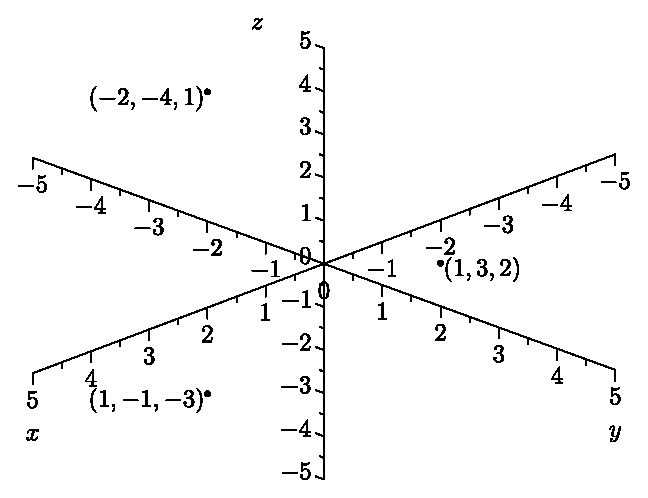
\includegraphics[scale=1]{figure02.eps}
\caption{Points in Cartesian three-space $\RR^3$}
\label{figure-three-space}
\end{figure}

As with $\RR^2$, the point \scalebox{0.7}{$\colvec{3}{a}{b}{c}
\in \RR^3$} is the unique point we find by moving $a$ units in the
$x$ direction, $b$ units in the $y$ direction and $c$ units in
the $z$ direction, as shown in Figure \ref{figure-three-space}.

When we visualize $\RR^2$, we conventionally write
the $x$ axis horizontally, with a positive direction to the
right, and the $y$ axis vertically, with a positive direction
upwards. There are similar conventions for $\RR^3$. 

\begin{defn}
A choice of axis directions in a visualization of $\RR^n$ 
is called an \emph{orientation}.
\end{defn}

While we can visualize $\RR^2$ and $\RR^3$ relatively easily and
efficiently, but we can't visualize any higher $\RR^n$. However,
that doesn't prevent us from working in higher dimensions. We need to
rely on the algebraic descriptions of vectors instead of the
drawings and visualizations of $\RR^2$ and $\RR^3$. 

In our visualizations of $\RR^2$ and
$\RR^3$, we see the different axes as fundementally
different perpendicular directions. We can think of $\RR^2$ as
the space with two independent directions and $\RR^3$ as the
space with three independent directions. Similarly, $\RR^4$ is
the space with four perpendicular, independent directions, even
though it is impossible to visualize such a thing. 
Likewise, $\RR^n$ is the space with $n$ independent directions. 

\section{Linear Operations}
\label{linear-operations}

\begin{figure}[t]
\centering
\includegraphics[width=12cm]{figure04.eps}
\caption{Visualizing Vector Addition}
\label{figure-vector-addition}
\end{figure}

The previous section built the environment for linear
algebra: $\RR^n$.  We want to know what operations we can
perform on $\RR^n$; there are several.

\begin{defn}
The \emph{sum} of two vectors $u$ and $v$ in $\RR^n$ is the
sum taken componentwise.
\begin{equation*}
u + v = \colvec{4}{u_1}{u_2}{\vdots}{u_n} +
\colvec{4}{v_1}{v_2}{\vdots}{v_n} = \colvec{4}{u_1 + v_1}{u_2
+ v_2}{\vdots}{u_n + v_n}
\end{equation*}
\end{defn}

Vector addition is visualized by putting the start of one
vector at the end of the other vector, as in Figure
\ref{figure-vector-addition}.  Note that we can only add two vectors
in the same dimension. We can't add a vector in $\RR^2$ to a
vector in $\RR^3$.

\begin{figure}[t]
\centering
\includegraphics[width=12cm]{figure05.eps}
\caption{Visualizing Scalar Multiplication}
\label{figure-scalar-multiplication}
\end{figure}

\begin{defn}
If $u$ is a vector in $\RR^n$ and $a \in
\RR$ is a real number, then the \emph{scalar multiplication} of
$u$ and $a$ is multiplication by $a$ in each component of $u$.
By convention, scalar multiplication is written with the
scalar on the left of the vector.
\begin{equation*}
au = a \colvec{4}{u_1}{u_2}{\vdots}{u_n} =
\colvec{4}{au_1}{au_2}{\vdots}{au_n}
\end{equation*}
\end{defn}

Multiplication stretches of shrink the vector while preserving
the direction or flipping if if the scalar is negative. This
is visualized in Figure \ref{figure-scalar-multiplication}. 

Though there will be other `multiplications' to come, we
generally say that we can't multiply vectors together in any way
reminiscent of numbers. Instead, we can only multiply by scalars.

Scalar multiplication also lets us define the difference
between vectors. 

\begin{figure}[t]
\centering
\includegraphics[scale=1]{figure06.eps}
\caption{Vector Subtraction and Distance Between Vectors}
\label{figure-vector-subtraction}
\end{figure}

\begin{defn}
The difference between two vectors $u$ and $v$ is the vector $u +
(-1)v$, defined using addition and scalar multiplication. This
works out to be componentwise subtraction.
\begin{equation*}
u - v = u + (-1) v= \colvec{4}{u_1}{u_2}{\vdots}{u_n} + (-1)
\colvec{4}{v_1}{v_2}{\vdots}{v_n} = \colvec{4}{u_1 - v_1}{u_2
- v_2}{\vdots}{u_n - v_n}
\end{equation*}
Subtraction is visualized as finding a vector that completes a
triangle, as in Figure \ref{figure-vector-subtraction}. 
\end{defn}

\begin{defn}
Given a set of scalars (such as $\RR$), whenever we find a
mathematical structure which has the two properties of
addition and scalar multiplication, we call the structure
\emph{linear}. $\RR^n$ is a linear space, because vectors
allow for addition and scalar multiplication.
\end{defn}

\begin{defn}
The \emph{length} of a vector $u$ in
$\RR^n$ is written $|u|$ and is given by a generalized form of
the Pythagorean rule for right triangles.
\begin{equation*}
|u| = \sqrt{u_1^2 + u_2^2 + \ldots + u_n^2}
\end{equation*}
This length is also called the \emph{norm} of the vector.
A vector of length one is called a \emph{unit vector}.
\end{defn}

If we think of vectors as directions from the origin towards a
point, this definition of length gives exactly what we expect:
the physical length of that arrow in $\RR^2$ and $\RR^3$.
Past $\RR^3$, we don't have a natural notion of length. This
definition serves as a reasonable generalization
to $\RR^4$ and higher dimensions which we can't
visualize. Note also that $|u| = 0$ only if $u$ is the zero
vector. All other vectors have positive length.

Often the square root is annoying and we find it convenient to
work with the square of length. 
\begin{equation*}
|u|^2 = u_1^2 + u_2^2 + \ldots + u_n^2
\end{equation*}
The notions of length and difference allow us to define the distance
between two vectors.

\begin{defn}
The \emph{distance between two vectors} $u$ and $v$ in $\RR^n$
is the length of their difference: $|u-v|$.
\end{defn}

You can check from the definition that $|u-v| = |v-u|$, so
distance doesn't depend on which comes first. If $|\cdot|$ were
absolute value in $\RR$, this definition would match the notion
of distance between numbers on the number line. 

\section{The Dot Product}
\label{dot-product}

Earlier we said that we can't multiply two vectors together.
However, there are operations similar to multiplication. The
following operation multiplies two vectors, but the result is
a scalar instead of another vector.

\begin{defn}
The \emph{dot product} or \emph{inner product} or \emph{scalar
product} of two vectors $u$ and $v$ is given by the following formula.
\begin{equation*}
u \cdot v = \colvec{4}{u_1}{u_2}{\vdots}{u_n} \cdot
\colvec{4}{v_1}{v_2}{\vdots}{v_n} = u_1 v_1 + u_2 v_2 + \ldots
+ u_n v_n
\end{equation*}
\end{defn}

We can think of the dot product as a scalar measure of the
similarity of direction between the two vectors. If the two
vectors point in a similar direction, their dot product is
large, but if they point in very different directions, their
dot product is small. However, we already have a measure, at
least in $\RR^2$, of this difference: the angle between two
vectors. Thankfully, the two measures of difference agree and
the dot product can be expressed in terms of angles.

\begin{defn}
The \emph{angle} $\theta$ between two non-zero vectors $u$ and
$v$ in $\RR^n$ is given by the equation
\begin{equation*}
\cos \theta = \frac{u \cdot v}{|u||v|}
\end{equation*}
We assume the angle between any two vectors is $\theta \in [0,
\pi]$. If $\theta > \pi$, then we can look at the other side
of the angle to get something between $0$ and $\pi$. 
\end{defn}

This definition matches with the definition of angles in
$\RR^2$ and $\RR^3$, which we can visualize. However, this
serves as a new definition for angles between vectors in all
$\RR^n$ when $n \geq 4$. Since we can't visualize those
spaces, we don't have a way of drawing angles and calculating
them with conventional trigonometry. This definition allows us
to extend angles in a completely algebraic way. 

\begin{defn}
Two vectors $u$ and $v$ in $\RR^n$ are called \emph{orthogonal}
or \emph{perpendicular} or \emph{normal} if $u \cdot v = 0$. 
\end{defn}

Now that we have some operations, it is useful to see how the
various operations interact. The following list shows
some interactions between addition, scalar multiplication,
length and the dot product. Some of these are easy to
establish from the definition and some take more work.

\begin{prop}
Let $u,v,w$ be vectors in $\RR^n$ and let $a$ be a scalar in $\RR$.
\begin{displaymath}
\begin{array}{rll}
u + v & = v + u & \hspace{1cm} \text{ Commutative Law for
Vector Addition} \\
a (u+v) & = au + av & \hspace{1cm} \text{ Distributive Law for
Scalar Multiplication}\\
u \cdot v & = v \cdot u & \hspace{1cm} \text{ Commutative
Law for the Dot Product}\\
u \cdot u & = |u|^2 & \\
u \cdot (v+w) & = u \cdot v + u \cdot w & \hspace{1cm} \text{
Distributive Law for the Dot Product}\\
u \cdot (av) & = (au) \cdot v = a (u \cdot v) \\
|u+v| & \leq |u| + |v| & \hspace{1cm} \ \text{ Triangle Inequality} \\
|au| & = |a||u| & 
\end{array}
\end{displaymath}
\end{prop}

The last line deserves some attention for the notation. When
we write $|a| |u|$, $|a|$ is an absolute value of a
real number and $|u|$ is the length of a vector. The fact
that they have the same notation is frustrating, but these
notations are conventional. 

\section{The Cross Product}
\label{cross-product}

The dot product is an operation which can be performed on any
two vectors in $\RR^n$ for any $n \geq 1$. 
There are no other conventional products that work
in all dimensions. However, there is a special product
that works in three dimensions. 

\begin{defn}
Let $u$ = \scalebox{0.7}{$\colvec{3}{u_1}{u_2}{u_3}$} and 
$v$ = \scalebox{0.7}{$\colvec{3}{v_1}{v_2}{v_3}$} be two 
vectors in $\RR^3$. The \emph{cross product} of $u$ and $v$ is
written $u \times v$ and defined by this formula:
\begin{equation*}
u \times v = \colvec{3}{u_2v_3 - u_3v_2}{u_3v_1 - u_1v_3}{u_1v_2 -
u_2v_1}
\end{equation*}
\end{defn}

The cross product differs from the dot product in several
important ways. First, it produces a new vector in $\RR^3$,
not a scalar. For this reason, when working in $\RR^3$, the
dot product is often refered to as the \emph{scalar product}
and the cross product as the \emph{vector product}. Second,
the dot product measures, in some sense, the similarity of two
vectors. The cross product measures, in some sense, the
difference between two vectors. The cross product has greater
magnitude if the vectors are closer to being perpendicular. If
$\theta$ is the angle between $u$ and $v$, the dot product was
expressed in terms of $\cos \theta$. This measures similarity,
since $\cos 0 = 1$. There is a similar identity for the cross
product.
\begin{equation*}
|u \times v| = |u||v| \sin \theta
\end{equation*}
This identity tells us that the cross product measures
difference in direction, since $\sin 0 = 0$. In particular,
this tells us that $|u \times u| = 0$, implying that $u \times
u = 0$ (the zero vector is the only vector which has zero
length). 

We can calculate a combination of the dot and cross products.
\begin{align*}
u \cdot (u \times v) & = 
\colvec{3}{u_1}{u_2}{u_3} \cdot \colvec{3}{u_2v_3 -
u_3v_2}{u_3v_1 - u_1v_3}{u_1v_2 - u_2v_1} \\
& = u_1u_2v_3 - u_1u_3v_2 + u_2u_3v_1 - u_2u_1v_3 + u_3u_1v_2
- u_3u_2v_1 = 0
\end{align*}

A similar calculation shows that $v \cdot (u \times v) = 0$.
Since a dot product of two vectors is zero if and only if the
vectors are perpendicular, the vector $v \times u$ is
perpendicular to both $u$ and $v$. This property turns out to
be very useful for describing planes in Sections
\ref{calculus-of-parametric-curves} and \ref{tangent-planes}.
There are two other identities for the cross product that we
will use in Chapter \ref{multivariable-functions}, which we
state here without proof. 

\begin{prop}
\label{prop-triple-cross-product}
Let $u,v,w \in \RR^3$ be vectors. 
\begin{equation*}
u \times (v \times w) = (u \cdot w) v - (u \cdot v) w
\end{equation*}
\end{prop}

\begin{prop}
\label{prop-cross-dot-product}
Let $u,v,w \in \RR^3$ be vectors. 
\begin{equation*}
u \cdot (v \times w) = v \cdot (w \times u) = w \cdot (u
\times v) 
\end{equation*}
\end{prop}

An important application of the cross product is describing
rotational motion. Linear mechanics describes the motion of
an object through space but rotational mechanics describes the
rotation of an object independently of its movement through
space. A force on an object can cause both kinds of movement,
obviously. The table below summarizes the parallel questions of
linear motion and rotational motion in $\RR^3$.

\begin{tabular}{l|l}
Linear Motion & Rotational Motion \\
\hline
Straight line in a vacuum & Continual spinning in a vacuum \\
Direction of motion & Axis of spin \\
Force & Torque \\
Momentum & Angular Momentum \\
Mass (resistance to motion) & Moment of Intertia (resistance
to spin) \\
Velocity & Frequency (Angular Velocity) \\
Acceleration & Angular Acceleration
\end{tabular}

How do we describe torque? If there is a linear force applied
to an object which can only rotate around an axis, and if
the linear force is applied at a distance $r$ from the axis,
we can think of the force $F$ and the distance $r$ as vectors.
The torque is then $\tau = r \times F$. Notice that $|\tau|
= |r||F| \sin \theta$, indicating that linear force
perpendicular to the radius gives the greatest angular
acceleration. That makes sense. If $F$ and $r$ are colinear,
that means we are pushing directly along the axis and no
rotation can occur. 

The use of cross products in rotational dynamics is extended
in many interesting ways. In fluid dynamics, local rotational
products of the fluid result in turbulence, helicity,
vorticity and similar effects. Tornadoes and
hurricanes are particularly extreme examples of vortices and
helices in the fluid which is the atmosphere. All the
descriptions of the force and motion of these vortices involve
cross products in the vectors describing the fluid. 

\section{Local Direction Vectors}
\label{local-directions}

We've already spoken about the distinction between elements of
$\RR^n$ as points and vectors. There is another important
subtlety that shows up all throughout vector geometry. In
addition to thinking of vectors as directions starting at the
origin, we can think of them as directions starting anywhere
in $\RR^n$. We call these local direction vectors.

For example, at the point \scalebox{0.7}{$\colvec{2}{2}{2}$} in $\RR^2$,
we could think of the local directions
\scalebox{0.7}{$\colvec{2}{1}{0}$} or
\scalebox{0.7}{$\colvec{2}{0}{1}$}. These
are not directions starting from the origin, but starting from
\scalebox{0.7}{$\colvec{2}{2}{2}$} \emph{as if that were the
origin}. 

\begin{figure}[t]
\centering
\includegraphics[scale=1]{figure08.eps}
\caption{Local Direction Vectors}
\label{figure-local-direction-vecdtors}
\end{figure}

Using vectors to define local directions is a particularly
useful tool. A standard example is camera location in a three
dimensional virtual environment. First, you need to know the
location of the camera, which is an ordinary vector starting
from the origin. Second, you need to know what direction the
camera is pointing, which is a local direction vector which
treats the camera location as the current origin.

One of the most difficult things about learning vector geometry
is becoming accustomed to local direction vectors. We don't
always carefully distinguish between vectors at the origin and
local direction vectors; often, the difference is implied and
it is up to the reader/student to figure out how the vectors
are being used. 

\section{Linear and Affine Subspaces}
\label{subspaces}

In addition to vectors, we want to consider various geometric
objects that live in $\RR^n$.

\begin{defn}
A \emph{linear subspace} of $\RR^n$ is a non-empty set of
vectors $L$ with two properties. 
\begin{smallitemize}
\item If $u,v \in L$ then $u+v \in L$.
\item If $u \in L$ and $a \in \RR$ then $av \in L$.
\end{smallitemize}
\end{defn}

These are the two basic operations on $\RR^n$:
we can add vectors and we can multiply by scalars. Linear
subspaces are just subsets where we can still perform both
operations and remain in the subset.

Geometrically, vector addition and scalar multiplication
produce flat objects: lines, planes, and their 
higher-dimensions analogues. Also, since we can take
$a=0$, we must have $0 \in L$. So linear subspaces can be
informally defined as flat subsets which include the origin.

\begin{defn}
An \emph{affine subspace} of $\RR^n$ is a non-empty set of
vectors $A$ which can be described as a sum $v+u$ where $v$ is
a fixed vector and $u$ is any vector in some fixed linear
subspace $L$. With some abuse of notation, we can write this
as
\begin{equation*}
A = u + L.
\end{equation*}
We think of affine subspaces as flat spaces that
may be offset from the origin. The vector $u$ is called the
\emph{offset vector}. Affine spaces include linear spaces,
since we can also take $u$ to be the zero vector and have
$A=L$. Affine objects are the lines, planes and higher
dimensional flat objects that may or may not pass through the
origin.
\end{defn}

Notice that we defined both affine and linear subspaces to be
non-empty. The empty set $\emptyset$ is \emph{not} a linear or
affine subspace. 

We need ways to algebraically describe linear and affine
substapces. There are two main approaches: loci and spans, but
these notes will only focus on loci. 

\section{Loci}
\label{loci}

\begin{defn}
Consider any set of linear equations in the variables
$x_1, x_2, \ldots, x_n$. The \emph{locus} in $\RR^n$ of this
set of equations is the set of vectors which satisfy
\emph{all} of the equations. The plural of locus is
\emph{loci}.
\end{defn}

In general, the equations can be of any sort. The unit circle
in $\RR^2$ is most commonly defined as the locus of the equation
$x^2 + y^2 = 1$. The graph of a function is the locus of the
equation $y = f(x)$. However, in linear algebra, 
we exclude curved objects. We're concerned with
linear/affine objects: things which are straight and flat.

\begin{defn}
A \emph{linear equation} in variables $x_1, x_2, \ldots x_n$
is an equation of the form
\begin{equation*}
a_1 x_1 + a_2 x_2 + \ldots + a_n x_n = c.
\end{equation*}
where $a_i$ and $c$ are real numbers
\end{defn}

\begin{prop}
Any linear or affine subspace of $\RR^n$ can be described as the
locus of some number of linear equations. Likewise, any locus
of any number of linear equations is either an affine subspace of
$\RR^n$ or the empty set.
\end{prop}

The best way to think about loci is in terms of
restrictions. We start with all of $\RR^n$ as the locus of no
equations, or of the equation $0=0$. There are no restrictions.
Then we introduce equations. Each equation is a restriction
on the available points. If we work in $\RR^2$, adding the
equation $x=3$ restricts us to a vertical line passing through
the $x$-axis at \scalebox{0.7}{$\colvec{2}{3}{0}$}. Likewise, if
we were to use the equation $y=4$, we would have a horizontal
line passing through the $y$-axis at
\scalebox{0.7}{$\colvec{2}{0}{4}$}. If we consider the locus
of \emph{both} equations, we have only one point remaining: 
\scalebox{0.7}{$\colvec{2}{3}{4}$} is the only point that satisfies both
equations. 

In this way, each additional equation potentially adds an
additional restriction and leads to a smaller linear or affine
subspace. The next three definitions give familiar names for
loci with one equation, hence one restriction.

\begin{defn}
A \emph{line} in $\RR^2$ is the locus of the equation $ax + by
= c$ for $a,b,c \in \RR$. In general, the line is affine. The
line is a linear subspace if $c=0$. 
\end{defn}

\begin{defn}
A \emph{plane} in $\RR^3$ is the locus of the linear equation
$ax + by + cz = d$. In general, the plane is affine. The
plane is a linear subspace if $d=0$. 
\end{defn}

If we think of a plane in $\RR^3$ as the locus of one linear
equation, then the important dimensional fact about a plane is
not that it has dimension two but that it has dimension one
less than its ambient space $\RR^3$. 

\begin{defn}
A \emph{hyperplane} in $\RR^n$ is the locus of one linear
equation: $a_1 x_1 + a_2 x_2 + \ldots + a_n x_n = c$. It has
dimension $n-1$. It is, in general, affine. The hyperplane is
a linear subspace if $c=0$. 
\end{defn}

\subsection{Intersection}
\label{intersection}

\begin{defn}
If $A$ and $B$ are sets, their intersection $A \cap B$ is the
set of all points they have in common. The intersection of
affine subspaces is also an affine subspace. If $A$ and $B$ are
both linear subspaces, the intersection is also a linear
subspace.
\end{defn}

\begin{example}
Loci can easily be understood as intersections. Consider the 
locus of two equations, say the example we have from $\RR^2$
before: the locus of $x=3$ and $y=4$. We defined this directly
as a single locus. However, we could just as easily think of
this as the intersection of the two lines given by $x=3$ and
$y=4$ seperately. In this way, it is the intersection of two
loci. Similarly, all loci are the intersection of planes or 
hyperplanes.
\end{example}

\section{Standard Forms}
\label{standard-forms}

Loci can also be defined via dot products. Consider,
again, the general linear equation in $\RR^n$.
\begin{equation*}
a_1 u_1 + a_2 u_2 + \ldots + a_n u_n = c
\end{equation*}
Let's think of the variables $u_i$ as the components of a
variable vector $u \in \RR^n$. We also have $n$ scalars
$a_i$ which we can treat as a constant vector $a \in \RR^n$. 

Then we can re-write the linear equation with dot products. 
\begin{equation*}
a_1 u_1 + a_2 u_2 + \ldots + a_n u_n =
\colvec{4}{a_1}{a_2}{\vdots}{a_n} \cdot
\colvec{4}{u_1}{u_2}{\vdots}{u_n} = 
a \cdot u = c
\end{equation*}
In this way, a linear equation specifies a certain dot product
value ($c$) with a fixed vector ($a$). A plane in $\RR^3$ is
given by the equation \scalebox{0.7}{$\colvec{3}{x}{y}{z}
\cdot \colvec{3}{a_1}{a_2}{a_3} = c$}. The plane is precisely
all vectors whose dot product with the vector \scalebox{0.7}{$
\colvec{3}{a_1}{a_2}{a_3}$} is the fixed number $c$.

If $c=0$, then we get \scalebox{0.7}{$\colvec{3}{x}{y}{z} \cdot
\colvec{3}{a_1}{a_2}{a_3} = 0$}. 
A linear plane is the set of all vectors which are
perpendicular to a fixed vector \scalebox{0.7}{
$\colvec{3}{a_1}{a_2}{a_3}$}. 

\begin{defn}
Let $P$ be a plane in $\RR^3$ determined by the equation 
\scalebox{0.7}{$\colvec{3}{x}{y}{z} \cdot
\colvec{3}{a_1}{a_2}{a_3} = c$}. 
The vector \scalebox{0.7}{$\colvec{3}{a_1}{a_2}{a_3}$} is
called the \emph{normal to the plane}. 

Let $H$ be a hyperplane in $\RR^n$ determined by the equation
\begin{displaymath}
u \cdot a = \colvec{4}{u_1}{u_2}{\vdots}{u_n} \cdot
\colvec{4}{a_1}{a_2}{\vdots}{a_n} = c 
\end{displaymath} 
The vector $a$ is called the \emph{normal to the hyperplane}. 
\end{defn} 

If $c=0$, the plane or hyperplane is perpendicular to the
normal. This notion of orthogonality still works when $c
\neq 0$. In this case, the normal is a \emph{local} perpendicular
direction from a point on the affine plane. Treating any such
point as a local origin, the normal points in a direction
perpendicular to all the \emph{local direction} vectors which
lie on the plane. 

Now we can build a general process for finding the
equation of a plane in $\RR^3$. Any time we have a point $p$
on the plane and two \emph{local direction vectors} $u$ and
$v$ which remain on the plane, we can find a normal to the
plane by taking $u \times v$. Then we can find the equation
of the plane by taking the dot product $p \cdot (u \times v)$
to find the constant $c$. 
\begin{displaymath}
\colvec{3}{x}{y}{z} \cdot (u \times v) = c
\end{displaymath} 
If we are given three points on a plane ($p$, $q$ and $r$), then
we can use $p$ as the local origin and construct the local
direction vectors as $q-p$ and $r-p$. The normal is $(q-p)
\times (r-p)$. In this way, we can construct the equation of a
plane given three points or a single point and two local
directions.

\section{Transformations of Euclidean Spaces}
\label{transformations}

After a good definition of the environment ($\RR^n$) and its
objects (lines, planes, hyperplanes, etc), the next
mathematical step is to understand the functions that live in
the environment and affect the objects.
First, we need to generalize the simple notion of a function
to linear spaces. In algebra and calculus, we worked with
functions of real numbers. These functions are rules $f: A
\rightarrow B$ which go between subsets of real numbers. The
function $f$ assigns to each \emph{number} in $A$ a unique
\emph{number} in $B$. They include the very familiar $f(x) =
x^2$, $f(x) = \sin (x)$, $f(x) = e^x$ and many others.

\begin{defn}
Let $A$ and $B$ be subsets of $\RR^n$ and $\RR^m$,
respectively. A \emph{function} between linear spaces is a
rule $f: A \rightarrow B$ which assigns to each \emph{vector} in
A a unique \emph{vector} in $B$.
\end{defn}

\begin{example}
We can define a function $f: \RR^3 \rightarrow \RR^3$ by 
$f(x,y,z) = (x^2, y^2, z^2)$. 
\end{example}

\begin{example}
Another function $f: \RR^3 \rightarrow \RR^2$ could be
$f(x,y,z) = (x-y, z-y)$. 
\end{example}

\begin{defn}
A \emph{linear function} or \emph{linear transformation} from
$\RR^n$ to $\RR^m$ is a function $f: \RR^n \rightarrow \RR^m$
such that for two vectors $u,v \in \RR^n$ and any scalar $a
\in \RR$, the function must obey two rules.
\begin{align*}
f(u+v) & = f(u) + f(v) \\
f(au) & = af(u)
\end{align*}
Informally, we say that the function respects the two main
operations on linear spaces: addition of vectors and
multiplication by scalars. If we perform addition before or after
the function, we get the same result. Likewise for scalar
multiplication.
\end{defn}

This leads to a very restrictive but important class of
functions. We could easily define linear algebra as a study of
these transformations. There is an alternative and equivalent
definition of linear transformation.

\begin{prop}
A function $f: \RR^n \rightarrow \RR^m$ is linear if and only
if it sends linear objects to linear objects.
\end{prop}

Under a linear transformation points, lines, planes are changed
to other points, lines, planes, etc. A line can't be bent into
an arc or broken into two different lines. Hopefully some
ideas are starting to fit together: the two basic operations
of addition and scalar multiplication give rise to flat
objects. Linear transformation preserve those operations, so
they preserve flat objects. Exactly \emph{how} they change
these objects can be tricky to determine.

Lastly, because of scalar multiplication, if we take $a
= 0$ we get that $f(0) = 0$. Under a linear transformation,
the origin is always sent to the origin. So, in addition to
preserving flat objects, linear transformation can't move the
origin. We could drop this condition of preserving the origin
to get another class of functions:

\begin{defn}
A \emph{affine transformation} from $\RR^n$ to $\RR^m$ is a
transformation that preserves affine subspaces. These
transformations preserve flat objects but may move the origin. 
\end{defn}

Though they are interesting, we don't spend much time with
affine transformations. They can always be realized as a linear
transformation combined with a shift or displacement of the
entire space by a fixed vector. Since shifts are relatively
simple, we can usually reduce problems of affine
transformations to problems of linear transformations.

Once we understood functions of real numbers we learned to
compose them. We do the same for linear transformations.

\begin{defn}
Let $f : \RR^n \rightarrow \RR^m$ and $g: \RR^m \rightarrow
\RR^l$ be linear transformations. Then $g \circ f : \RR^n
\rightarrow \RR^l$ is the linear transformation formed by first
applying $f$ and then $g$. Note that the $\RR^m$ has to match:
$f$ outputs to $\RR^m$, which is the input for $g$. Also note
that the notation is written right-to-left: In $g \circ f$, the
transformation $f$ happens first, followed by $g$. This new
transformation is called the \emph{composition} of $f$ and $g$.
\end{defn}

\section{Transformations of $\RR^2$ or $\RR^3$}
\label{transformations-r2-r3}

It is useful for us to specialize to transformations $\RR^2
\rightarrow \RR^2$, in order to build experience and intuition.
As we noted above, linear transformations preserve flat
objects. What can we do to $\RR^2$ that preserves lines and
preserves the origin? 

\begin{prop}
There are five basic types of linear transformation of $\RR^2$.
\end{prop}

\begin{itemize}
\item \emph{Rotations} about the origin (either
clockwise or counter-clockwise) 
preserve lines. We can't rotate around any other point,
since that would move the origin. Since we can choose any
angle, there are infinitely many such rotations. Also, since
rotating by $\theta$ radians clockwise is the same as $2\pi -
\theta$ radians counter-clockwise, we typically choose to only
deal with counter-clockwise rotations. Counter-clockwise
rotations are considered positive and clockwise rotations are
considered negative.
\item \emph{Reflections} over lines through the origin 
preserve lines. The line of reflection must be a line  through
the origin or else the reflection will move the origin.
\item \emph{Skews} are a little tricker to visualize. A skew
is a transformation that takes either veritcal or horizontal
lines (but not both) and tilts them diagonally. It changes
squares into parallelograms. The tilted lines are still
lines, so it is a linear transformation.
\item \emph{Dialations} are transformation which stretch or
shink in various directions. 
\item \emph{Projections} are transformations which collapse
$\RR^2$ down to a line through the origin. Two important
exampels are projection onto either axis. Projection onto the
$x$ axis sends a point $(a,b)$ to $(a,0)$, removing the $y$
component. Likewise, projection onto the $y$ axis sends a point
$(a,b)$ to $(0,b)$, removing the $x$ component. In a similar
manner, we can project onto any line though the origin by
sending each point to the closest point on the line. Finally,
there is the projection to the origin which sends all points to
the origin.
\end{itemize}

All linear transformation of $\RR^2$ are generated by
composition of transformations of these five types.

We can also specialize to transformations of $\RR^3$, though it
is not as easy to give a complete account of the basic types.
However, all of the types listed for $\RR^2$ generalize.

\begin{itemize}
\item Rotations in $\RR^3$ are no longer about the origin.
Instead, we have to choose an axis. Any line through the origin
will do for an axis of rotation. Any rotation in $\RR^3$ is
determined by an axis of rotation and an angle of rotation about
that axis.
\item Reflections are also altered: instead of reflecting over a
line, we have to reflect over a plane through the origin. Any
plane through the origin determines a reflection.
\item Skews are similarly defined: one or two directions are
fixed and the remaining directions are tilted.
\item Dialations are also similar, though we have three possible
directions in which to stretch or compress.
\item Like $\RR^2$, we can project onto the origin, sending
everything to zero, or onto a line, sending every point to the
closest point on a line. Examples include projection
onto the axes. However, we can also project onto planes.
Sending $(a,b,c)$ to $(a,b,0)$, for example, removes the $z$
coordinate; this is projection onto the $xy$ plane.
\end{itemize}

\section{Matrix Representation}
\label{matrix-representation}

Matrices are used to encode linear transformations. We define
an action to show how a matrix can act on a vector.

\begin{defn}
Let $A = a_{ij}$ be a $m \times n$ matrix and let $v$ be a vector in
$\RR^n$. There is an action of $A$ on $v$, written
$Av$, which defines a new vector in $\RR^m$. That action is
given in the following formula.
\begin{displaymath}
\left( 
\begin{matrix}
a_{11} & a_{12} & \cdots & a_{1n} \\
a_{21} & a_{22} & \cdots & a_{2n} \\
\vdots & \vdots & \vdots & \vdots \\
a_{n1} & a_{n2} & \cdots & a_{nn} 
\end{matrix}
\right)
\colvec{4}{v_1}{v_2}{\vdots}{v_n}
= 
\colvec{4}
{a_{11}v_1 + a_{12}v_2 + \ldots + a_{1n}v_n} 
{a_{21}v_1 + a_{22}v_2 + \ldots + a_{2n}v_n} 
{\vdots}
{a_{n1}v_1 + a_{n2}v_2 + \ldots + a_{nn}v_n} 
\end{displaymath}
\end{defn}

This is a bit troubling to work out in general. Let's see
what it looks like slightly more concretely in $\RR^2$ and
$\RR^3$.
\begin{align*}
\left( 
\begin{matrix}
a & b \\
c & d 
\end{matrix}
\right)
\colvec{2}{x}{y} 
& = 
\colvec{2}{ax + yb}{cx + dy} \\
\left( 
\begin{matrix}
a & b & c \\
d & e & f \\
g & h & i 
\end{matrix}
\right)
\colvec{3}{x}{y}{z} 
& = 
\colvec{3}
{ax + by + cz}{dx + ey + fz}{gx + hy + iz}
\end{align*}

In this way, all $m \times n$ matrices determine a method of
sending vectors in $\RR^n$ to $\RR^m$: a function $\RR^n
\rightarrow \RR^m$. It is not at all obvious from the
definition, but this connection completely describes linear
transformations.

\begin{prop}
If $A$ is a $m \times n$ matrix, then the associated function
defined by the matrix action is a linear function $\RR^n
\rightarrow \RR^m$. Moreover, all linear functions $\RR^n
\rightarrow \RR^m$ can be encoded this way. Finally, each
linear function is encoded uniquely, i.e., each $m \times n$
matrix corresponds to a different transformation.
\end{prop}

In this way, the set of linear transformation $\RR^n
\rightarrow \RR^m$ is \emph{exactly} the same as the set of $m
\times n$ matrices. This is a very powerful result: 
in order to understand linear transformations of
Euclidean space, we only have to understand matrices and their
properties. 

\begin{example}
First, we had the zero matrix: all coefficients are zero. 
\begin{displaymath}
\left( 
\begin{matrix}
0 & 0 & 0 \\
0 & 0 & 0 \\
0 & 0 & 0 
\end{matrix}
\right)
\colvec{3}{x}{y}{z} 
= 
\colvec{3}
{0x + 0y + 0z}{0x + 0y + 0z}{0x + 0y + 0z}
= 
\colvec{3}{0}{0}{0} 
\end{displaymath}
The zero matrix corresponds to the transformation that sends
all vectors to the origin. 
\end{example}

\begin{example}
We also had the identity matrix: ones one the diagonal and
zeros elsewhere.
\begin{displaymath}
\left( 
\begin{matrix}
1 & 0 & 0 \\
0 & 1 & 0 \\
0 & 0 & 1 
\end{matrix}
\right)
\colvec{3}{x}{y}{z} 
= 
\colvec{3}
{1x + 0y + 0z}{0x + 1y + 0z}{0x + 0y + 1z}
= 
\colvec{3}{x}{y}{z} 
\end{displaymath}
The identity matrix corresponds to the transformation which
doesn't change anything. Appropriately, we called this the
identity transformation. 
\end{example}

\begin{example}
Diagonal matrices only have non-zero entires on the diagonal.
\begin{displaymath}
\left( 
\begin{matrix}
a & 0 & 0 \\
0 & b & 0 \\
0 & 0 & c 
\end{matrix}
\right)
\colvec{3}{x}{y}{z} 
= 
\colvec{3}
{ax + 0y + 0z}{0x + by + 0z}{0x + 0y + cz}
= 
\colvec{3}{ax}{by}{cz} 
\end{displaymath}
This is a dialation: the $x$ direction is stretched by the
factor $a$, the $y$ direction by the factor $b$ and the $z$
direction by the factor $c$. 
\end{example}

\section{Matrices in $\RR^2$}
\label{matrices-in-r2}

We defined five types of basic
transformations in $\RR^2$. Let's give them explicit
description in terms of matrices.

\begin{itemize}
\item The first class was rotations. To be linear, they needed
to fix the origin, so they needed to be rotations about the
origin. Rotation by $\theta$ (counter-clockwise, as per the
standard convention) is given by the following matrix.
\begin{equation*}
\left( \begin{matrix}
\cos \theta & - \sin \theta \\
\sin \theta & \cos \theta
\end{matrix} \right) 
\end{equation*}
In particular, rotations by $\pi/2$, $\pi$ and $3\pi/2$ radians
are given by the following matrices, respectively.
\begin{equation*}
\left( \begin{matrix}
0 & -1 \\ 1 & 0 
\end{matrix} \right) 
\hspace{1cm}
\left( \begin{matrix}
-1 & 0 \\ 0 & -1
\end{matrix} \right) 
\hspace{1cm}
\left( \begin{matrix}
0 & 1 \\ -1 & 0 
\end{matrix} \right) 
\end{equation*}
\item The second class was reflections. To preserve the
origin, they needed to be reflections over a line through the
origin. In general, take $\colvec{2}{a}{b}$ to be a non-zero
\emph{unit} vector in $\RR^2$.  Reflection over this line in
the direction $\colvec{2}{a}{b}$ is given by the following
matrix.
\begin{equation*}
\left( \begin{matrix}
a^2 - b^2 & 2ab \\
2ab & b^2 - a^2 
\end{matrix} \right) 
\end{equation*}
In particular, reflections over the $x$-axis, the $y$-axis,
the line $y=x$ and the line $y=-x$ are given by the following
matrices, respectively.
\begin{equation*}
\left( \begin{matrix}
1 & 0 \\ 0 & -1 
\end{matrix} \right) 
\hspace{1cm}
\left( \begin{matrix}
-1 & 0 \\ 0 & -1 
\end{matrix} \right) 
\hspace{1cm}
\left( \begin{matrix}
0 & 1 \\ 1 & 0 
\end{matrix} \right) 
\hspace{1cm}
\left( \begin{matrix}
0 & -1 \\ -1 & 0 
\end{matrix} \right) 
\end{equation*}
\item The next set of matrices are skews. We're not going to
give a general form, but consider the following two matrices.
\begin{equation*}
\left( \begin{matrix}
1 & 1 \\ 0 & 1 
\end{matrix} \right) 
\hspace{1cm}
\left( \begin{matrix}
1 & 0 \\ 1 & 1 
\end{matrix} \right) 
\end{equation*}
The first matrix is a skew by one in the positive $y$
direction, and the second is a skew by one in the positive $x$
direction. Both change squares into parallelograms. We can
generalize this slighty: the following matrices are skews in
$y$ and $x$ by the factor $a$, respectively.
\begin{equation*}
\left( \begin{matrix}
1 & a \\ 0 & 1 
\end{matrix} \right) 
\hspace{1cm}
\left( \begin{matrix}
1 & 0 \\ a & 1 
\end{matrix} \right) 
\end{equation*}
\item Dialations were the next class. To dialate by $a$ in the
$x$ direction and by $b$ in the $y$ direction, we use a
diagonal matrix.
\begin{equation*}
\left( \begin{matrix}
a & 0 \\ 0 & b 
\end{matrix} \right) 
\end{equation*}
\item Finally, we have projections. To project onto the line
in the direction $\colvec{2}{a}{b}$, we have the following
matrix.
\begin{equation*}
\frac{1}{a^2 + b^2}\left( \begin{matrix}
a^2 & ab \\ ab & b^2
\end{matrix} \right) 
\end{equation*}
In particular, projections onto the $x$ axis, the $y$ axis, the
line $y=x$ and the line $y=-x$ are given by the following
matrices, respectively.
\begin{equation*}
\left( \begin{matrix}
1 & 0 \\ 0 & 0 
\end{matrix} \right) 
\hspace{1cm}
\left( \begin{matrix}
0 & 0 \\ 0 & 1 
\end{matrix} \right) 
\hspace{1cm}
\frac{1}{2} \left( \begin{matrix}
1 & 1 \\ 1 & 1 
\end{matrix} \right) 
\hspace{1cm}
\frac{1}{2} \left( \begin{matrix}
1 & -1 \\ -1 & 1 
\end{matrix} \right) 
\end{equation*}
Finally, projection to the origin is given by the zero matrix.
\begin{equation*}
\left( \begin{matrix}
0 & 0 \\ 0 & 0 
\end{matrix} \right) 
\end{equation*}
\end{itemize}

\section{Determinants}
\label{determinants}

Linear transformations are defined by their symmetries: they
preserve linear subspaces and linear operations. We use
associated matrices to understand these transformations.
Matrices are an algebraic description, so that questions of
transformation can be turned into algebraic problems.  Now
that we have the algebraic description of transformations as
matrices, we want to investigate what else the matrix can tell
us about the transformation. In this section, we are asking
two questions in particular.

First, what does the transformation do to the size of objects?
I choose the vague word `size' intentionally because we work
in various dimensions. In one dimension, size is length. In
two dimensions, size is area. In three dimensions, size is
volume. And in higher dimensions, we have some extended
notion of volume that fits that dimension; we can call this
hyper-volume. It is important to note that size depends on
the ambient dimension. A square in $\RR^2$ has some area,
some non-zero size. But if we have a flat square somewhere in
$\RR^3$, it has no volume, therefore no substantial size in
that space. 

Second, what does the transformation do to the orientation of
an object? Orientating is slightly trickier to understand
than size, so we will define it for each dimension. In
$\RR$, orientation is direction: moving in the positive
or negative direction along the numberline. There are only two
directions of movement, so two orientations. If we have a
transformation of $\RR$, we can ask if it changes or preserves
these directions. In $\RR^2$, instead of moving in line, we
think of moving in closed loops or paths. These paths can be
clockwise or counter-clockwise. Then we can ask if a
transformation changes clockwise loops into other clockwise
loops or into counter-clockwise loops. This gives a notion of
orientation in $\RR^2$. In $\RR^3$, orientation relates to
the relative position of positive directions. The axis system
in $\RR^3$ is, conventionally, given by a right-hand-rule. It
we know the $x$ and $y$ directions, the right-hand-rule
indicates the positive $z$ direction. Then we can ask where
these three directions go under a transformation and if a
right-hand-rule still applies. If it does, we preserve the
orientation. If it doesn't, and a left-hand-rule would work
instead, the transformation reverses orientation. In higher
dimension, there are other extentions of the notion of
orientation. In each case, the question is binary: a
transformation either preserves or reverses orientation..

\begin{defn}
Let $M$ be a square $n \times n$ matrix. The
\emph{determinant} of $M$ is a real number, written $\det M$,
with two properties. Its absolute value $|\det M|$ measures
the effect that $M$ has on size (length, area, volume,
hyper-volume). Its sign (positive or negative) measures the
effect on orientation; if the sign is positive, orientation is
preserved, and if the sign is negative, orientation is
reversed.
\end{defn}

That definition is all well and good, but we need to show 
that such a thing can be constructed. The next section
gives an algorithm for building determinants.

\section{Calculation of Determinants}
\label{calculation-of-determinants}

The determinant of a (square) matrix is constructed
recursively, starting with $2 \times 2$ matrices. We'll often
use the notation of replacing the curved braces 
with straight lines to indicate determinants. 
\begin{equation*}
\det \left( \begin{matrix} a & b \\ c & d \end{matrix} \right)
= 
\left| \begin{matrix} a & b \\ c & d \end{matrix} \right| =
ad-bc
\end{equation*}

\begin{example}
For the matrix $\left( \begin{matrix} 1 & -3 \\ 2 & -1
\end{matrix} \right)$, the determinant is $(1)(-1) - (2)(-3) =
-1 + 6 = 5$. Therefore, we know that this matrix multiplies
all areas by a factor of $5$ and preserves orientation.
\end{example}

\begin{example}
Recall that rotations in $\RR^2$ all have a standard form.
\begin{equation*}
\left( \begin{matrix} 
\cos \theta & - \sin \theta \\ \cos \theta & \sin \theta
\end{matrix} \right) 
\end{equation*}
The determinant of this expression is $(\cos \theta)(\cos
\theta) - (-\sin \theta)(\sin \theta) = \cos^2 \theta + \sin^2
\theta = 1$. So all rotations preserve area and preserve
orientation. This makes sense: spinning a shape around the
origin does not change or area, nor does it change clockwise
paths around an object into counter-clockwise paths. 
\end{example}

\begin{example}
Recall we also had a standard form for reflections
(we assumed that \scalebox{0.7}{$\colvec{2}{a}{b}$} is unit vector
when we define reflections, so $a^2 + b^2 = 1$).
\begin{equation*}
\left( \begin{matrix}
a^2 - b^2 & 2ab \\ 2ab & b^2 - a^2
\end{matrix} \right) 
\end{equation*}
The determinant here is $( ( a^2 - b^2)(b^2
- a^2) - (2ab)(2ab)) = ( -a^4 - b^4 + 2a^2
 b^2 - 4a^2 b^2) = (-a^4 - b^4 - 2a^2) = -(a^2 + b^2)^2$
which simplifies to $-1$. This also makes sense, since area is
unchanged but orientation is reversed. A reflection doesn't
change area, but we expect that clockwise paths, when flipped,
become counter-clockwise paths.
\end{example}

\begin{defn}
The algorithm for calculating determinants in general is
called \emph{Co-Factor Expansion}. It is a recursive algorithm
that reduces determinant calculation to determinants of
smaller square matrices, eventually down to $2 \times 2$
matrices.
\end{defn}

Co-factor expansion procceds in this way: We choose \emph{any} column or
row of the matrix. We take the coefficients from that column
or row. For each of the coefficients, we multiply that
coefficient by the detminant of the matrix formed by removing
both the columnn and row containig that coefficient. Then we
add up the determinants of these small matrices multiplied by
matching coefficients, with a pattern of $\pm$ signs. That
pattern of $\pm$ signs is a checkerboard pattern, as in this
$5 \times 5$ matrix:
\begin{equation*}
\left( \begin{matrix}
+ & - & + & - & + \\
- & + & - & + & - \\
+ & - & + & - & + \\
- & + & - & + & - \\
+ & - & + & - & + \\
\end{matrix} \right) 
\end{equation*}
That's a hard algorithm to intuit from the formal description.
Let's do a number of examples. 

\begin{example}
Here is a $3 \times 3$ example where we do co-factor expansion
on the first row.
\begin{align*}
\left| 
\begin{matrix}
5 & -2 & 0 \\ -3 & 3 & -2 \\ 1 & -5 & 3 
\end{matrix} 
\right|
& = 
(+1) 5 \left| 
\begin{matrix}
3 & -2 \\ -5 & 3 
\end{matrix} 
\right|
+ (-1) (-2)
\left| 
\begin{matrix}
-3 & -2 \\ 1 & 3 
\end{matrix} 
\right|
+ (+1) (0)
\left| 
\begin{matrix}
-3 & 3 \\ 1 & -5 
\end{matrix} 
\right| \\
& = 5 ((3)(3) - (-2)(-5)) + 2( (-3)(3) - (-2)(1)) + (0) (-3)(-5) -
(3)(1) \\
& = 5 (-1) + 2 (-7) = - 19
\end{align*}
\end{example}

\begin{example}
In this example, we do cofactor expansions along the second
column.
\begin{align*}
\left| 
\begin{matrix}
4 & 0 & -8 \\ -1 & -2 & 3 \\ 5 & 0 & 0 
\end{matrix} 
\right| 
& = 
0 (-1) \left| 
\begin{matrix}
-1 & 3 \\ 5 & 0 
\end{matrix} 
\right|
+ (+1)(-2)
\left| 
\begin{matrix}
4 & -8 \\ 5 & 0 
\end{matrix} 
\right|
+ (0) (-1)
\left| 
\begin{matrix}
4 & -8 \\ -1 & 3
\end{matrix} 
\right| \\
& = 0 ((-1)(-) - (3)(5)) - 2((4)(0) - (5)(-8)) + 0 ((4)(3) -
(-8)(-1)) \\
& = 0 - 2(40) + 0 = -80
\end{align*}
\end{example}

\begin{example}
Here is a $4 \times 4$ example, where we have to do cofactor
expansion twice. The first expansion gives us four $3 \times
3$ matrices. We do cofactor expansion on each to give the $2
\times 2$ matrices that we know how to calculate. We start
with cofactor expansion along the first column.
\begin{align*}
& \left| 
\begin{matrix}
4 & -1 & -1 & 6 \\
0 & -3 & 3 & -2 \\
0 & 1 & 1 & -2 \\
-2 & 0 & 0 & 3 
\end{matrix} 
\right| \\
& = 
+ (+1) (4)
\left| 
\begin{matrix}
-3 & 3 & -2 \\
1 & 1 & -2 \\
0 & 0 & 3 
\end{matrix} 
\right|
+ (-1) (0)
\left| 
\begin{matrix}
-1 & -1 & 6 \\ 1 & 1 & -2 \\ 0 & 0 & 3 
\end{matrix} 
\right| \\
& \hspace{1cm} + (+1) (0)
\left| 
\begin{matrix}
-1 & - 1 & 6 \\ -3 & 3 & -2 \\ 0 & 0 & 3
\end{matrix} 
\right|
+ (-1) (-2)
\left| 
\begin{matrix}
-1 & -1 & 6 \\
-3 & 3 & -2 \\
1 & 1 & -2 
\end{matrix} 
\right| \\
& = 
+ 4
\left| 
\begin{matrix}
-3 & 3 & -2 \\
1 & 1 & -2 \\
0 & 0 & 3 
\end{matrix} 
\right|
- 0
+ 0
+ 2
\left| 
\begin{matrix}
-1 & -1 & 6 \\
-3 & 3 & -2 \\
1 & 1 & -2 
\end{matrix} 
\right| \\
\intertext{Then we do cofactor expansion again on both of the
$3 \times 3$ matrices. We use the third row of the first
matrix, and the first column of the second matrix.}
& = 
4 \left[ (+1)(0)
\left| 
\begin{matrix}
3 & -2 \\ 1 & -2 
\end{matrix} 
\right|
+ (-1)(0)
\left| 
\begin{matrix}
-3 & -2 \\ 1 & -2 
\end{matrix} 
\right|
+ (+1)(3)
\left| 
\begin{matrix}
-3 & 3 \\ 1 & 1 
\end{matrix} 
\right| \right] \\
& \hspace{1cm} + 
2 \left[ 
(+1)(-1)
\left| 
\begin{matrix}
3 & -2 \\ 1 & -2 
\end{matrix} 
\right|
+ (-1)(-3)
\left| 
\begin{matrix}
-1 & 6 \\ 1 & -2 
\end{matrix} 
\right|
+ (+1)(1)
\left| 
\begin{matrix}
-1 & 6 \\ 3 & -2 
\end{matrix} 
\right| \right] \\
& = 4 \left[ 
(0)((3)(-2) - (1)(-2)) + (0)((-3)(-2) - (1)(-2)) +
(3)((-3)(1) - (3)(1))
\right] \\
& \hspace{1cm} + 2 \left[
(-1)((3)(-2) - (-2)(1)) + (3)((-1)(-2) - (3)(6)) +
(1)((-1)(-2) - (3)(6)) 
\right] \\
& = 4 \left[ (3)(-3-3) \right] 
+ 2 \left[ (-1)(-6 + 2) + (3)(2 - 6) + (2 - 18)) \right] \\
& = -72 + 8 - 24 - 32 = -120
\end{align*}
\end{example}

You may have noticed that we always choose a row or column with a
maximum number of zeros for co-factor expansion. This is
a useful technique, since it removes extra calculation.

If we did cofactor expansion of an arbitrary $3 \times 3$
matrix, we would get a direct expression for the
determinant.
\begin{equation*}
\left| \begin{matrix}
a & b & c \\ d & e & f \\ g & h & i
\end{matrix} \right| = aei - ahf - bdi + bfg + cdh - ceg
\end{equation*}
We could use this formula for $3 \times 3$ matrices, if we
wished. We could do the same for larger matrices, but it
starts to get quite complicated. The computational complexity
of the recursive determinant algorithm grows very quickly. For
a $3 \times 3$ matrix, we had 3 recursions to $2 \times 2$
matrices, each with $2$ multiplication terms in the
determinant, giving $6$ terms. Each term was the multiple of
three coefficients, giving $12$ total multiplications. For a
$4 \times 4$, the recursions gives $24$ terms, each with $4$
coefficients, so $24\cdot 3 = 72$ multiplications. For a $5
\times 5$ matrix, we recurse five times to a $4 \times 4$
matrix, for $120$ terms each with $5$ coefficients, which is
$120 \cdot 4 = 600$ multiplications. The pattern continues:
there are $n!$ terms in the determinant of a $n \times n$
matrix, each with $n$ coefficient, for $n! (n-1)$
multiplications. This is computationally terrifying, making
determinants of large matrices computationally very difficult.

\chapter{Non-Linear Coordinate Systems}
\label{non-linear-coordinates}

One way of thinking of transformations of $\RR^n$ is as
changes of coordinates.  In $\RR^2$, with standard coordinates
$x,y$, we can think of a linear transformation, say $u = x+v$
and $v=x-v$, as a new system of coordinates. We can describe
points, loci, and any other objects in terms of $u$ and
$v$ just as well as in terms of $x$ and $y$. The
transformation tells us how to go between the two sets of
coordinates. 

All the linear transformations mentioned in the previous
section (at least those which preserve dimension) are changes
of coordinates. In this section, we look at changing to new
coordinates in stranger ways; in particular, we look as
non-linear transformations.

\section{Polar Coordinates}
\label{polar-coordinates}

In $\RR^2$, the most common non-linear coordinate system is polar
coordinates. Polar coordinates describe $\RR^2$ in terms of
circles and rays instead of the conventional lines of
Cartesian coordinates. The system has two parameters
(coordinates): $r$ and $\theta$. $r$, the radius, is the
distance of a point from the origin. We have $r \in
[0, \infty)$, since that distance can't be negative. If we
draw a ray from the origin to a point, $\theta$
is the angle between that line and the $x$ axis, with the
convention that $\theta \in [0, 2\pi)$. 

\begin{figure}[ht]
\centering
\includegraphics[width=12cm]{figure26.eps}
\caption{Polar Coordinates}
\label{figure-polar-coordinates}
\end{figure}

We would like to be able to move between Cartesian and polar
coordinates. To that end, we need to describe $x$ and $y$
in terms of $r$ and $\theta$, and vice-versa. The
relationships are just trigonometry.
\begin{equation*}
x = r \cos \theta \hspace{2cm} y = r \sin \theta
\end{equation*}
The reverse direction is also trigonometry.
\begin{equation*}
r = \sqrt{x^2 + y^2} \hspace{2cm} \tan \theta = \frac{y}{x}
\implies \theta = \arctan \frac{y}{x}
\end{equation*}
If $x$ is zero, then $\tan \theta$ is undefined, but $\theta$
will be $\pi/2$ or $3\pi/2$, depending on whether $y$ is
positive or negative. If $x$ and $y$ are both zero, at the
origin, the angle is not defined at all.

Loci in $\RR^2$ are equations in $x$ and $y$. The simplest
such loci were $x=c$, which is a vertical line, and $y=c$,
which is a horizontal line. We get loci in $\RR^2$ in terms
of $r$ and $\theta$ as well. $r=c$ is a circle: the shape
with any angle and a fixed radius. $\theta =c$ is a ray: the
shape with a fixed angle and any radius.  Figures
\ref{figure-polar-locus1} thought \ref{figure-polar-locus4} show some
exammples of loci in polar coordinates.

To translate between loci in polar coordinates and loci in
Cartesian coordinates is simply a matter of replacement. The
line $x=4$ in Cartesian coordinates becomes $r\cos \theta = 4$
or $\cos \theta = \frac{r}{4}$. The circle $x^2 + y^2 =1 $
becomes $r^2 \cos^2 \theta + r^2 \sin^2 \theta = 1$, which is
simply $r^2 = 1 \implies r=1$. The polar locus $r=\theta$
becomes $\sqrt{x^2 + y^2} = \arctan \frac{y}{x}$.

\begin{figure}[t]
\centering
\includegraphics[width=5cm]{figure27.eps}
\caption{$r = \theta$}
\label{figure-polar-locus1}
\end{figure}

\begin{figure}[t]
\centering
\includegraphics[width=5cm]{figure28.eps}
\caption{$r = |\sin \theta|$}
\label{figure-polar-locus2}
\end{figure}

\begin{figure}[t]
\centering
\includegraphics[width=5cm]{figure29.eps}
\caption{$r = 1 + \sin \theta$}
\label{figure-polar-locus3}
\end{figure}

\begin{figure}[t]
\centering
\includegraphics[width=5cm]{figure30.eps}
\caption{$r = 3 \sin 2 \theta$}
\label{figure-polar-locus4}
\end{figure}

\section{Spherical and Cylindrical Coordinates}
\label{spherical-cylindrical}

In $\RR^3$, there two are similar coordinate systems.
Cylindrical coordinates use polar coordinates in the $xy$
plane and leave the $z$ coordinate unchanaged. The
transformations are again given by trigonometry. 
\begin{align*}
x & = r \cos \theta \\
y & = r \sin \theta \\
z & = z
\end{align*}
We can invert the transformation.
\begin{align*}
r & = \sqrt{x^2 + y^2} \\
\theta & = \arctan \left( \frac{y}{x} \right) \\
z & = z
\end{align*}
These are called cylindrical coordinates since the equation $r=c$
gives rise to a infinitely tall cylinder. $r=c$ in the $xy$
plane is a circle, as before. The $z$ coordinate is left free, so
the circle can be located at any $z$ value. That infinitely
tall stack of circles is a cylinder.

Spherical coordinates uses a sphere the same way that polar
coordinates uses a circle. There is a radius term $r$, which
measure the distance from a point to the origin in $\RR^3$.
$r$ determines the size of a sphere on which the point is
located. After determining a sphere, to find a specific point
on the sphere, we use a system which is similar to the system
of longitude and latitude on the surface of the earth.
$\theta$ is the same as longitude, but with $\theta \in [0,
2\pi)$ instead of counting positively in both east and west
directions. The $0$ line of longitude is the line that passes
through the positive $x$ axis. $\phi$ is co-latitude instead
of latitude: it starts at $0$ at the top of the sphere and
counts down to $\pi$ radians at the bottom of the sphere. The
transformations involve some tricky trigonometry in $\RR^3$.
\begin{align*}
x & = r \sin \phi \cos \theta \\
y & = r \sin \phi \sin \theta \\
z & = r \cos \phi
\end{align*}
We can invert the transformation.
\begin{align*}
r & = \sqrt{x^2 + y^2 + z^2} \\
\theta & = \arctan \left( \frac{y}{x} \right) \\
\phi & = \arctan \left( \frac{\sqrt{x^2 + y^2}}{z} \right) 
\end{align*}
The equation $r=c$ in spherical coordinates gives a sphere. 

\chapter{Parametric Curves}
\label{parametric-curves}

\section{Introduction}
\label{parametric-curves-introduction}

The major goal of this course is the extension of calculus to
functions with multiple variable inputs and/or outputs. In
Chapter \ref{vector-geometry}, we introduced linear
transformation, which were function $\RR^n \rightarrow \RR^m$,
but we would like to also investigate non-linear functions.
Parametric curves are the first foray; we allow a single-input
function to have a multi-variable non-linear output.  We
interpreted parametric curves as vectors or positions in some
euclidean space; as such, parametric curves are used to talk
about motion through space.  The calculus of parametric curves
is a way to understand the physics of such motion, covering
both linear and angular velocity and acceleration in a nice,
holistic approach. When considering parametric curves, we
should imagine the movement of point-like objects through
space under the influence of various forces.  Projectiles with
gravity and air friction is one imporant example; the motions
of planets, moons and satellite under gravity is another. 

Considering the motion of stellar objects around a large
gravity source (such as planets, asteroids and comets around
the sun), we will use the caluculus of parametric curves to
derive Kepler's laws of planetary motion from the basic
assumptions of Newtonian mechanics. Kepler's laws predate
Newton, but they were simply observed, not derived. The fact
that Newton's physics, with multivariable calculus, can
recover these observations from first principles of motion and
gravity is a major accomplishment of that theory. In order to
cover Kepler's laws in full, these notes also include 
descriptions of conics as parametric curves.

\section{Vector Valued Functions}
\label{vector-valued-functions}

\begin{defn}
Let $A$ be a subset of $\RR$. A \emph{vector valued function}
is a function $f: A \rightarrow \RR^n$ for $n \geq 2$. It has
a single-variable real input, but outputs a vector in some
higher dimensional space. A vector valued function can be
written as a vector of individual functions.
\begin{equation*}
f(t) = (f_1(t), f_2(t), \ldots, f_n(t))
\end{equation*}
The function $f_i$ are called the \emph{component functions}
of the vector-valued function. In $\RR^2$, the components
will often be written $(x(t), y(t))$, and similarly in $\RR^3$,
$(x(t), y(t), z(t))$.
\end{defn}

The single-variable component functions allow us to quickly
extend many notions from single-variable calculus to
vector-valued functions.

\begin{defn}
The \emph{limit} of a vector valued function is simply the
limit of each component. 
\begin{equation*}
\lim_{t \rightarrow a} f(t) = \left( 
\lim_{t \rightarrow a} f_1 (t), 
\lim_{t \rightarrow a} f_2 (t), 
\ldots, 
\lim_{t \rightarrow a} f_2 (t) \right)
\end{equation*}
\end{defn}

Recall that a single variable function $f(t)$ is continuous at
$a \in \RR$ if
\begin{equation*}
\lim_{x \rightarrow a} f(x) = f(a).
\end{equation*}

\begin{defn}
A vector-valued function is \emph{continuous} if and only if each
component function is continuous. 
\end{defn} 

\begin{defn} 
The \emph{derivative} of a vector valued function $f: A
\rightarrow \RR^n$ is calculated in each component.
\begin{equation*}
\frac{df}{dt} = f^\prime(t) = \left( \frac{df_1}{dt},
\frac{df_2}{dt}, \ldots, 
\frac{df_n}{dt} \right) 
\end{equation*}
We state this explicitly, for $f(x) = (x(t),y(t))$ with values
in $\RR^2$.
\begin{equation*}
f^\prime(t) = \frac{d}{dt} f(t) = \left( \frac{dx}{dt},
\frac{dy}{dt}\right)
\end{equation*}
Likewise, we give the explicit form for $f(t) = (x(t),
y(t),z(t))$ with values in $\RR^3$. 
\begin{equation*}
f^\prime(t) = \frac{d}{dt} f(t) = \left( \frac{dx}{dt},
\frac{dy}{dt}, \frac{dz}{dt} \right) 
\end{equation*}
\end{defn}

\begin{defn} 
Similarly, the integral of $f$ is defined componentwise.
\begin{equation*}
\int f(t) dt = \left( \int f_1(t) dt, \int f_2(t) dt, \ldots, 
\int f_n(t) dt \right)
\end{equation*}
We state this explicitly, for $f(x) = (x(t),y(t))$ with values
in $\RR^2$. 
\begin{equation*}
\int f(t) dt = \left( \int x(t) dt, \int y(t) dt \right)
\end{equation*}
Likewise, we give the explicit form for $f(x) =
(x(t),y(t),z(t))$ with values in $\RR^3$. 
\begin{equation*}
\int f(t) dt = \left( \int x(t) dt, \int y(t) dt, \int z(t)
dt \right)
\end{equation*}
\end{defn}

The result of a derivative or integral of a vector valued
function is still a vector. This may seem odd from the
viewpoint of first year calculus, where derivatives and
integrals measured quantifiable geometric properties, such as
slopes of tangent lines and areas under curves. Since the
answers here are vectors instead of scalars, we will
eventually reconsider those interpretations. A major challenge
in extending calculus to several variables is the need to
re-adjust our interpretation and intuition concerning
derivatives and integrals. The derivative is no longer the
slope of a tangent line. 

\section{Parametric Curves}
\label{parametric-curves-definition}

\begin{figure}[t]
\centering
\includegraphics[width=5cm]{figure10.eps}
\caption{The curve $\gamma(t) = (\cos t, \sin t)$}\
\label{figure-parametric-curve1}
\end{figure}

\begin{figure}[t]
\centering
\includegraphics[width=5cm]{figure11.eps}
\caption{The curve $\gamma(t) = \left( \frac{1}{t} , t
\right)$}
\label{figure-parametric-curve2}
\end{figure}

\begin{defn}
A parametric curve in $\RR^n$ is a continuous function $\gamma
:[a,b] \rightarrow \RR^n$, that is, a continuous vector-valued
function defined on an interval. As is convention, we will
typically use the symbol $\gamma$ for an arbitrary parametric
curve.
\end{defn} 

We identify a parametric curve with its image: that is, we think
of a curve as a decription of the set of points in $\RR^n$ which
are the output of the curve. In this interpretation, we think
of the curve as describing motion along this set: we start at
the point $\gamma(a) \in \RR^n$ and move along the curve, ending
at $\gamma(b) \in \RR^n$ when we get to the end of the domain.

The continuity condition is important, since a parametric
curve is a connected path. We could think of vector-valued
functions which jump around, but these don't really fit the
notion of a curve. Continuity is also necessary for
differentiability and we will assume (in order to avoid
restating it multiple times) that all our parametric curves
are differentiable.

For visualizing parametric curves, we graph only the output or
image of the curve. There is never a $t$ axis in any of these
graphs; instead, the variable $t$ is the parameter of movement
along the curve. 

\begin{example}
The curve $\gamma(t) = (\cos t, \sin t)$, for $t \in [0,
2\pi]$ traces out a circle, as in Figure
\ref{figure-parametric-curve1}. 
\end{example}

Notice that we defined this curve on the domain $[0, 2\pi]$. If
we extend this domain, the curve just starts to retrace over
the circle. It's good to observe that parametric curves can
self-intersect and trace over themselves many times.

\begin{figure}[t]
\centering
\includegraphics[width=5cm]{figure12.eps}
\caption{The curve $\gamma(t) = (\cos 2t, \sin t)$}
\label{figure-parametric-curve3}
\end{figure}

\begin{figure}[t]
\centering
\includegraphics[width=5cm]{figure13.eps}
\caption{The logarithmic spiral}
\label{figure-parametric-curve4}
\end{figure}

\begin{example}
The curve $\gamma(t) = \left(\frac{1}{t}, t \right)$
on the domain $t \in \left[\frac{1}{5},5 \right]$ traces part
of the graph of $f(x) = \frac{1}{x}$, as in Figure
\ref{figure-parametric-curve2}.
\end{example}

Notice that this parametric curve is the graph of a function,
specifically the function $f(x) = \frac{1}{x}$ between $x =
\frac{1}{5}$ and $x=5$. Parametric curves where one of the
components is just $t$ can be interpreted as graphs of
functions.

\begin{example}
The curve $\gamma(t) = (\cos 2t, \sin t)$ on the domain
$t \in [0, 2\pi]$ oscilates faster in the $x$ direction than
in the $y$ direction, as in Figure \ref{figure-parametric-curve3}.
\end{example}

\begin{example}
A spiral in $\RR^2$ is a parametric curve of the form
$\gamma(t) = (f(t) \cos t, f(t) \sin t)$ where $f(t)$ is a
monotonic function. It resembles the circle, but the radius is
either increasing or decreasing as the curve traces around the
circle. The curve $\gamma(t) = (2e^{\frac{t}{4}} \cos t,
2e^{\frac{t}{4}} \sin t)$ is a logarithmic spiral, as in
Figure \ref{figure-parametric-curve4}.
\end{example}

\begin{figure}[t]
\centering
\includegraphics[width=5cm]{figure14.eps}
\caption{The archimedian spiral}
\label{figure-parametric-curve5}
\end{figure}

\begin{figure}[t]
\centering
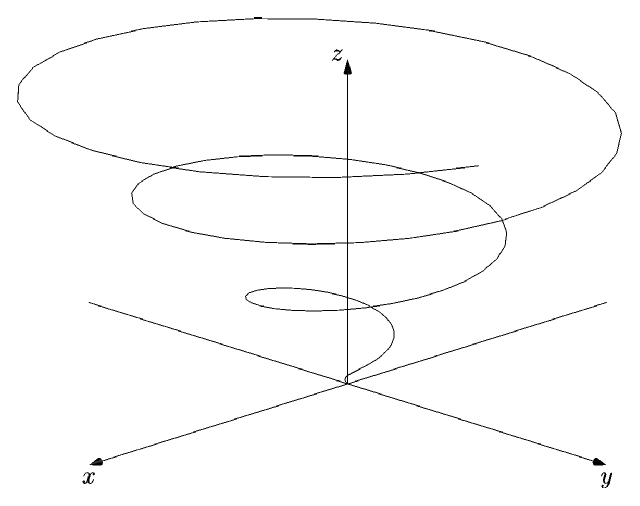
\includegraphics[width=5cm]{figure15.eps}
\caption{The curve $\gamma(t) = (t \cos t, t \sin t, t)$}
\label{figure-parametric-curve6}
\end{figure}

\begin{example}
The curve $\gamma(t) = (t \cos t, t \sin t)$ is the
archimedian spiral, as in Figure \ref{figure-parametric-curve5}.
\end{example}

\begin{example}
The curve $\gamma(t) = (t\cos t, t\sin t,t)$ on $[0,20]$ is a
spiral in $\RR^3$, as in Figure \ref{figure-parametric-curve6}.
\end{example}

\subsection{Parametric Curves in Polar Coordinates}
\label{parametric-curves-polar-coordinates}

Once we are comfortable with changing coordinate systems, we can
use any coordinate system we wish to describe parametric curves.
For example, polar coordinates in $\RR^2$ are well suited to
describing any kind of object that is circular in some
sense. Curves in polar coordinates are given as $\gamma(t) =
(r(t), \theta(t))$ instead of $\gamma(t) = (x(t),y(t))$. The
circle in parametric coordinates is $\gamma(t) = (1, t)$; if
we write the components individually, we could write 
$\theta(t) = t$ and $r(t) = 1$. The logarithmic spiral has
components $\theta(t) = t$ and $r(t) = 2e^{\frac{t}{4}}$. The
archimedian spiral has components $\theta(t) = t$ and $r(t) = t$.

\section{Parametrization}
\label{parametrization}

\subsection{Varied Parametrizations}
\label{varied-parametrization}

\begin{figure}[t]
\centering
\includegraphics[width=12cm]{figure17.eps}
\caption{The graph of a parabola as a parametric curve}
\label{figure-parametric-parabola}
\end{figure} 

There are many ways to describe the same shape by a parametric
curve. 

\begin{example}
\label{example-four-parametrizations}
Consider the following curves.
\begin{align*}
\gamma_1(t) = \left( t^2, t^4 \right) & \hspace{1.0cm} t \in [0,
4] \\
\gamma_2(t) = \left( t, t^2 \right) & \hspace{1.0cm} t \in [0,
16] \\
\gamma_3(t) = \left( \sqrt{t}, t \right) & \hspace{1.0cm} t \in [0,
256] \\
\gamma_4(t) = \left( 5t, 25t^2 \right) & \hspace{1.0cm} t \in
\left[0, \frac{16}{5} \right] \\
\end{align*}
All four of these have exactly the same parabolic image. They
all describe the same curve, shown in Figure
\ref{figure-parametric-parabola}.
\end{example}

\subsection{Reparametrization}
\label{reparametrization}

Since the same shape can have many different parametrizations,
we want a process to switch between them. This process is called
reparametrization. 

\begin{defn} 
Let $\gamma(t): [a,b] \rightarrow \RR^n$ be a parametric
curve with coordinates $(\gamma_1(t), \ldots,
\gamma_n(t))$. A \emph{reparametrization} of $\gamma$ is a
monotonic increasing function $t = t(u)$ expressing the
parameter $t$ in terms of a new parameter $u$. We replace $t$
by the function $t(u)$ to give a parametric curve in terms of
$u$: $\gamma(u) = (\gamma_1(t(u)), \gamma_2(t(u)), \ldots,
\gamma_n(t(u)))$. 
\end{defn}

\begin{example}
The unit circle in $\RR^2$ is parametrized by
$\gamma(t) = (\cos t, \sin t)$. If $t = 3u$ then $\gamma(u) =
(\cos 3u, \sin 3u)$ is a reparametrization of the same circle.
The first parametrization finishes a revolution in $t \in [0,
2\pi]$, but multiplication by $3$ in the second parametrization
means that a full revolution is completed in $u \in [0,
2\pi/3]$ -- that is, the second parametrization moves along the
circle three times as fast. 

Many reparametrizations of the circle are possible.
\begin{align*}
\text{If } t = \frac{u}{3} & \text{ then } \gamma(u) = \left(
\cos \frac{u}{3}, \sin \frac{u}{3} \right) \\
\text{If } t = u^2 & \text{ then } \gamma(u) = \left(
\cos u^2, \sin u^2 \right) \\
\text{If } t = \sqrt{u} & \text{ then } \gamma(u) = \left(
\cos \sqrt{u}, \sin \sqrt{u} \right) 
\end{align*}
Even though the shape of the curve is the same, the
parametrization affects the rate movement along the curve. 
\end{example}

\subsection{Arc Length}
\label{arc-length}

\begin{figure}[t]
\centering
\includegraphics[width=12cm]{figure19.eps}
\caption{Arclength setup by approximation}
\label{figure-arclength-approximation}
\end{figure} 

Our goal in this section is to produce a formula describing
the length of a parametric curve. We approximate this length
by breaking up a curve $\gamma$ into a series of straight
lines. In order to visualize the process, we work in $\RR^2$
for the moment, as in Figure \ref{figure-arclength-approximation}.

For each straight line segment, if we know $\Delta y$ and
$\Delta x$, then the length of the segment is $\sqrt{\Delta
x^2 + \Delta y^2}$.
We approximate the total length of the curve by adding up
the lengths of these segments.
\begin{equation*}
L \cong \sum \sqrt{\Delta x^2 + \Delta y^2}
\end{equation*}
If we take the limit of this process, breaking the curve into
smaller and smaller pieces, we get a Riemann sum which defines a
definite integral. In the limit, the $\Delta$ terms become the
infinitesimals $dy$ and $dx$. 
\begin{equation*}
L = \int_a^b \sqrt{dx^2 + dy^2}
\end{equation*}
Both $x$ and $y$ depend on $t$, so we can change this to a
integral in $t$.
\begin{equation*}
L = \int_a^b \sqrt{ \left( \frac{dx}{dt} \right)^2 + \left(
\frac{dy}{dt} \right)^2 } dt 
\end{equation*}
The same arguments work in any $\RR^n$, leading to the general
result.

\begin{prop}
Let $\gamma(t): [a,b] \rightarrow \RR^n$ be a parametric
curve. Let $\gamma_1(t), \gamma_2(t), \ldots, \gamma_n(t)$ be
the components. The length of the parametric curve is
calculated by this integral.
\begin{equation*}
L = \int_a^b \sqrt{ \left( \frac{d\gamma_1}{dt} \right)^2 
+ \left( \frac{d\gamma_2}{dt} \right)^2 + \ldots + 
+ \left( \frac{d\gamma_n}{dt} \right)^2 } dt 
\end{equation*}
\end{prop}

\begin{example}
The asteroid is the parametric curve $\gamma(t) = (\cos^3 t,
\sin^3 t)$ for $t \in [0,2\pi]$, shown in Figure
\ref{figure-asteroid}. We want to calculate its arclength.

\begin{figure}[ht]
\centering
\includegraphics[width=7cm]{figure20.eps}
\caption{The Asteroid}
\label{figure-asteroid}
\end{figure}

\begin{align*}
L & = \int_a^b \sqrt{ \left( \frac{dx}{dt} \right)^2 + \left(
\frac{dy}{dt} \right)^2 } dt \\
& = \int_0^{2\pi} \sqrt{ (-3 \cos^2 t (\sin t))^2 + (3 \sin^2
t (\cos t))^2} dt \\
& = \int_0^{2\pi} \sqrt{ 9 \cos^4 t \sin^2 t + 9 \sin^4
t \cos^2 t} dt \\
& = \int_0^{2\pi} |3 \sin t \cos t | \sqrt{ \sin^2 + \cos^2 t} dt \\
& = \int_0^{2\pi} |3 \sin t \cos t | dt \\
\end{align*}

The absolute value here causes trouble. A convenient way to
drop it is to notice that both $\sin t$ and $\cos t$ are positive on
$[0, \pi/2]$. That range covers a quarter of the asteroid and
the asteroid is symetric, so we can calculate the length of that
quarter and multiply by 4.
\begin{equation*}
L = 4\int_0^{\frac{\pi}{2}} 3 \sin t \cos t dt = 
6 \int_0^{\frac{\pi}{2}} \sin 2t = \left. -3\cos 2t
\right|_0^{\frac{\pi}{2}} = 6
\end{equation*}
\end{example}

\begin{example} 
In $\RR^3$, consider the helix $\gamma(t) = (\cos t, \sin t,
t)$. On the domain $t \in [0, 8\pi]$, the helix makes four
revolutions. We calculate its arclength.
\begin{equation*}
L = \int_0^{8\pi} \sqrt{ \sin^2 t + \cos^2 t + 1} dt =
\int_0^{8\pi} \sqrt{2} dt = 8 \sqrt{2} \pi
\end{equation*}
\end{example}

\subsection{Parametrization by Arclength}
\label{parametrization-by-arclength}

Our arclength 
calculation determins the length of the whole curve. However,
we can also ask for the length of pieces of the curve.

\begin{defn}
Let $\gamma(t): [a,b] \rightarrow \RR^n$ be a parametric curve
with components $(\gamma_1(t), \ldots, \gamma_n(t))$.  The
\emph{arclength function} $s(t): [a,b] \rightarrow [0,
\infty)$ is defined by this integral.
\begin{equation*}
s(t) = \int_a^t \sqrt{ \left( \frac{d\gamma_1(u)}{du} \right)^2 
+ \left( \frac{d\gamma_2(u)}{du} \right)^2 + \ldots + 
+ \left( \frac{d\gamma_n(u)}{du} \right)^2 } du 
\end{equation*}
The letter $s$ is conventional notation for the arclength
function. 
\end{defn}

The arclength function measures the length of the curve as a
function of the parameter; it is simply the distance travelled
along the curve. For example, if $t \in [0,10]$, then $s(3)$
is the distance along the  curve from $\gamma(0)$
to $\gamma(3)$, $s(5)$ is the distance the curve has covered
from $\gamma(0)$ to $\gamma(5)$, $s(8)$ is the distance along
the curve from $\gamma(0)$ to $\gamma(8)$ and so on.  Since
$s$ depends on $t$ outside the integral, we have to choose a
temporary variable $u$ for inside the integral; in the
integral, $t$ is simply repalced with $u$.

We want to use the arclength function to reparametrize curve.
The process has three steps.
\begin{smallparts}
\item We calculate the arclength fuction $s(t)$ by
integration.
\item We invert the arclength function. Arclength is always an
increasing function, so it is always invertible. We write the
inverse as $t(s)$. 
\item We use the inverse of the arclength function to
reparametrize by replacing $t$ with $t(s)$. 
\end{smallparts}

\begin{defn}
Let $\gamma(t) : [a,b] \rightarrow \RR^n$ be a parametric
curve. Let $s(t)$ be the arclength function, with $t(s)$ its
inverse. The reparametrization $\gamma(t(s))$ is called the
\emph{parametrization by arclength}. It is the unique
parametrization where the parameter is the distance along the
curve. 
\end{defn}

\begin{example}
\label{example-helix-reparametrized}
Consider the helix $\gamma(t) = (2 \cos t, 2 \sin t, 4t)$
defined for $t > 0$, shown in Figure \ref{figure-helix}.

\begin{figure}[t]
\centering
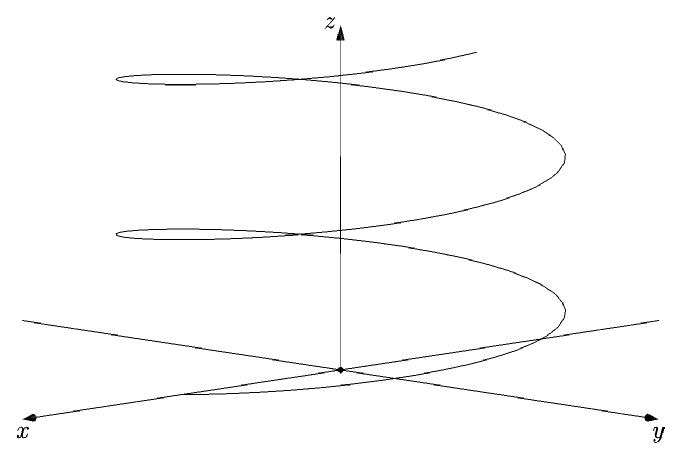
\includegraphics[width=12cm]{figure21.eps}
\caption{The helix $\gamma(t) = (2 \cos t, 2 \sin t, 4t)$}
\label{figure-helix}
\end{figure} 

We calculate the arclength function.
\begin{align*}
s(t) & = \int_0^t \sqrt{x^\prime(u)^2 + y^\prime(u)^2 +
z^\prime(u)^2} du \\
& = \int_0^t \sqrt{4\sin^2 u + 4 \cos^2 u + 4^2} du = \int_0^t
\sqrt{20} du = t \sqrt{20}
\end{align*}
The arclength function is $s = t \sqrt{20}$; the inverse is $t =
\frac{s}{\sqrt{20}}$. We replace $t$ with $t(s)$ in 
$\gamma(t)$.
\begin{equation*}
\gamma(s) = \left( 2 \cos \left( \frac{s}{\sqrt{20}} \right),
2 \sin \left( \frac{s}{\sqrt{20}} \right),
\frac{4s}{\sqrt{20}} \right) 
\end{equation*}
\end{example}

\section{Calculus of Parametric Curves}
\label{calculus-of-parametric-curves}

\subsection{Tangents}
\label{tangents}

Parametric curves are vector-valued functions, so they have
derivatives as defined earlier. Since we consider
parametric curves as motion through $\RR^n$, the derivative
has a related interpretation.

\begin{defn} Let $\gamma(t): [a,b] \rightarrow \RR^n$ be a
parametric curve. Its derivative $\gamma^\prime(t)$ is called
the \emph{tangent vector} to the parametric curve.
\end{defn}

This tangent is no longer the slope of a tangent line from
single-variable claculus. It is a vector, which we treat as a
local direction vector along the curve. At $\gamma(a)$,
$\gamma^\prime(a)$ points in the local
direction of movement. The notion of a derivative as a
tangent direction replaces old notion of the derivative as the
slope of the tangent line. 

\begin{figure}[t]
\centering
\includegraphics[width=12cm]{figure16.eps}
\caption{A tangent vector to the logarithmic spiral}
\label{figure-logarithmic-spiral-tangent}
\end{figure} 

\begin{example}
Consider the logarithmic spiral $\gamma(t) =
(e^{\frac{t}{4}}\sin t, e^{\frac{t}{4}}\cos t)$ on the domain
$t \in \RR$. We calculate its derivative.
\begin{equation*}
\gamma^\prime(t) = \left( e^{\frac{t}{4}} \cos t + \frac{1}{4}
e^{\frac{t}{4}} \sin t, -e^{\frac{t}{4}} \sin t + \frac{1}{4}
e^{\frac{t}{4}} \cos t \right)
\end{equation*}
Evaluating at $t=0$ at the point of the curve $\gamma(0) =
(0,1)$, the derivative or tangent vector to the curve is
$\gamma^\prime(0) = (1,\frac{1}{4})$. 

This spiral is moving outwards; we can see how the
tangent vector points in the direction of movement as the curves
goes through $(0,1)$. Figure \ref{figure-logarithmic-spiral-tangent}
shows how we treat the tangent as a local direction vector: it
points from $\gamma(0) = (0,1)$, not from the origin.
\end{example}

\begin{figure}[t]
\centering
\includegraphics[width=12cm]{figure18.eps}
\caption{Length of tangent vectors depending on
parametrization}
\label{figure-tangent-lengths}
\end{figure} 

\begin{example}
Consider the four parametrizations of the graph of the parabola
introduced in Example \ref{example-four-parametrizations}  and their
tangents to the point $(1,1)$.
\begin{align*}
\gamma_1^\prime (t) = \left( 2t, 4t^3 \right) & \hspace{1.0cm} t=1 
\text{ at } (1,1) \implies
\gamma_1^\prime (1) = \left( 2, 4 \right) & \\
\gamma_2^\prime (t) = \left( 1, 2t \right) & \hspace{1.0cm} t=1
\text{ at } (1,1) \implies
\gamma_2^\prime (1) = \left( 1, 2 \right) & \\
\gamma_3^\prime (t) = \left( \frac{1}{2\sqrt{t}}, 1 \right) &
\hspace{1.0cm} t=1 \text{ at } (1,1) \implies
\gamma_3^\prime (1) = \left( \frac{1}{2} , 1 \right) & \\
\gamma_4^\prime (t) = \left( 5, 50t \right) & \hspace{1.0cm} t
= \frac{1}{5} \text{ at } (1,1) \implies
\gamma_4^\prime (\frac{1}{5}) = \left( 5, 10 \right) &\\
\end{align*}
All of these tangent vectors are multiples of the vector
$(1,2)$, but they have different lengths, as seen in Figure
\ref{figure-tangent-lengths}.
\end{example}

We said the tangent vector indicated the instantaneous
direction of motion. The tangent vector also has a length,
independent of the direction. The length of the tangent vector
measures the speed of the curve going through that point. If
the movement along the curve is very fast, the tangent vector
will have a large length; if the movement along the curve is
slow, the tangent vector will be shorter.

For the parametrizations of the graph of the parabolic, we can
see that the direction of the tangent is independent of the
parametrization, but the length of the tangent is entirely
dependent on the parametrization. The parametrization which
move more quickly along the curve have longer tangents.

Often it is useful to only consider the tangent direction. 

\begin{defn}
If $\gamma^\prime(t)$ is the tangent vector of a parametric
curve, the \emph{unit tangent vector} is the unique vector of
length one in the same direction as $\gamma^\prime(t)$. It is
often written $T(t)$. To calculate the unit tangent, we simply
take the tangent vector and divide by its length.
\begin{equation*}
T(t) = \frac{\gamma^\prime(t)}{|\gamma^\prime(t)|}
\end{equation*}
\end{defn}

\begin{example}
In the logarithmic spiral, the tangent vector was $\gamma^\prime(0) =
(1, \frac{1}{4})$. We calculate the length of this vector.
\begin{equation*}
\left|\left(1,\frac{1}{4}\right)\right| = \sqrt{ 1 +
\frac{1}{16}} = \frac{\sqrt{17}}{4}
\end{equation*}
Then we can calculate the unit tangent.
\begin{equation*}
T(t) = \frac{\gamma^\prime(t)}{|\gamma^\prime(t)|} =
\frac{4}{\sqrt{17}}\left( 1, \frac{1}{4} \right) = \left(
\frac{4}{\sqrt{17}},\frac{1}{\sqrt{17}} \right) 
\end{equation*}
\end{example}

\begin{example}
In the various parametrizations of the graph of the
parabola, the tangent direction was $(1,2)$, so the unit
tangent is $\left( \frac{1}{\sqrt{5}},
\frac{2}{\sqrt{5}} \right)$.
\end{example}

\subsection{Tangents in Non-Linear Coordinates}
\label{tangents-non-linear-coords}

Tangents are a Cartesian notion. If our curve is given in a
different coordinate systems, we still want the word `tangent'
to mean the Cartesian tangent. Cartesian tangents cary the
interepretation we want: the direction of motion. Therefore,
to find tangent in other coordinate systems, we relate them
back to Cartesian coordinates. In polar coordinates, we have
$x = r \cos \theta$ and $y = r \sin \theta$. If $r$ and
$\theta$ depend on $t$, then we can differentiation these
expressions using the product rule. 
\begin{align*}
x^\prime & = r^\prime \cos \theta - r \sin \theta \theta^\prime
\\
y^\prime & = r^\prime \sin \theta + r \cos \theta \theta^\prime 
\\
\gamma^\prime(t) & = (r^\prime \cos \theta - r \sin \theta
\theta^\prime, r^\prime \sin \theta + r \cos \theta
\theta^\prime)
\end{align*}

\subsection{Arclength and Tangents}
\label{arclength-and-tangents}

There are some very natural connections between tangents and
arclength which relate to the intepretation of parametric
curves as movement through space.  Let's return to the arc
length formula (in $\RR^2$, for simplicity).
\begin{equation*}
L = \int_a^b \sqrt{x^\prime(t)^2 + y^\prime(t)^2} dt
\end{equation*}
The tangent vector is $\gamma^\prime(t) =
(x^\prime(t), y^\prime(t))$, so this integrand in the
arclength formula is nothing more
than the length of the tangent vector. This lets us rewrite
the arclength formula.
\begin{equation*}
L = \int_a^b |\gamma^\prime(t)| dt
\end{equation*}
This hopefully makes intuitive sense -- the length of the tangent
vector measures the speed of the curve. To get length (the
distance travelled), we integrate the speed of movement.

An nice event occurs when we differentiate the arclength
function $s(t)$. The fundamental theorem of calculus allows us
to differentiate an integral.
\begin{equation*}
\frac{d}{dt} s(t) = \frac{d}{dt} \int_a^t |\gamma^\prime(u)| du
= |\gamma^\prime (t)|
\end{equation*}
The derivative of the arclength function is the length of
the tangent vector, which represents the speed of movement
along the curve. To get speed, we differentiate length.

Both of these observations generalize the relationship between
distance and speed from single variable calculus. In that
forum, the relationship was relatively direct: if $d(t)$ was
distance, then $d^\prime(t)$ was speed and if $v(t)$ was speed
then $\int v(t) dt$ was distance. The idea here is exactly the
same, but since the movement is much more complicated, going
through multi-dimensional space, we need more complicated
definitions and notations to access the idea.

\begin{example} 
Recall the parametrization by arclength of the helix in
$\RR^3$ in Example \ref{example-helix-reparametrized}.
\begin{equation*}
\gamma(s) = \left( 2 \cos \left( \frac{s}{\sqrt{20}} \right),
2 \sin \left( \frac{s}{\sqrt{20}} \right),
\frac{4s}{\sqrt{20}} \right) 
\end{equation*}
Let's calculate the speed in this parametrization by
arclength. 
$|\gamma^\prime(s)|$:
\begin{align*}
|\gamma^\prime(s)| & = \sqrt{ x^\prime(s)^2 + y^\prime(s)^2 +
z^\prime(s)^2} \\
& = \sqrt{ \left( \frac{-2}{\sqrt{20}} \sin \left(
\frac{s}{\sqrt{20}} \right) \right)^2 + \left( \frac{2}{\sqrt{20}} 
\cos \left( \frac{s}{\sqrt{20}} \right) \right)^2
+ \left( \frac{4}{\sqrt{20}} \right)^2} \\
& = \sqrt{\frac{4}{20} \left( \cos^2 \left(
\frac{5}{\sqrt{20}} \right) + \sin^2 \left( \frac{5}{\sqrt{20}}
\right) \right) + \frac{16}{20} } = \sqrt{ \frac{4}{20} +
\frac{16}{20}} = 1
\end{align*}
We find that the speed is constantly one. This turns out to be
generally true.
\end{example}

\begin{prop}
Let $\gamma(t): [a,b] \rightarrow \RR^n$ be a parametric
curve. Our of all the possible reparametrizations of $\gamma$,
the parametrization by arclength has three properties.
\begin{smallitemize}
\item It is the unique parametrization with constant speed of 1.
\item It is the unique parametrization where all tangent vectors
have length 1.
\item It is the unique parametrization where the parameter
measures distance along the curve.
\end{smallitemize}
\end{prop}

These properties are very useful and convenient. In the
remainder of this chapter, we will make frequent use of the
parametrization by arclength; it serves as our default
parametrization. We can do this since the parametrization by
arclength always exists and is unique. Having a special,
default parameter allows us to make good definitions which
will be independent of the choice of parametrization. (In
practice, the parametrization by arclength can be extremely
difficult to actually calculate. For theoretical results,
however, this difficulty isn't relevant).

\subsection{Curvature and Torsion}
\label{curvature-and-torsion}

The tangent vector for a parametric curve measures the speed
and direction of movement along the curve. Speed and direction
are good information, but not enough to complete describe
motion in multiple dimensions. In particular, the tangent
vector gives the direction but doesn't say how direction is
changing. This section builds up the notions of curvature and
torsion, which will complete a full description of th
echanging directions of movement. In this section, we
exclusively work in $\RR^3$.

In $\RR^3$, I want to classify three types of movement.
\begin{smallitemize}
\item Straight motion: the direction is fixed and only speed
varies.
\item Curving motion in a plane: motion is fixed to a plane,
but the direction can change and curve in the plane.
\item Twisting motion: the most general motion, where in
addition to curving in a plane, we can also twist away from
the plane.
\end{smallitemize}
Throughout this section, let $\gamma(t): [a,b] \rightarrow
\RR^3$ be a curve in three dimensions. Recall we already have
the tangent $\gamma^\prime(t)$ and the unit tangent $T(t)$.
If the curve is parametrized by arc length, we will use the
parameter $s$ and write $\gamma(s)$. In this case, the tangent
is already a unit vector, so $T(s) = \gamma^\prime(s)$. We
will usually start our definition using the parmetrization by
arclength, to ensure they are independent of
parametrizations.

\begin{defn}
The \emph{curvature} of $\gamma(s)$ is a scalar $\kappa(s)$
which measure how quickly the curve is turning. 
\begin{equation*}
\kappa(s) = \left| \frac{dT(s)}{ds} \right|
\end{equation*}
\end{defn}

We can think of turning as a change in the direction of the
unit tangent $T(s)$. It is a scalar, not showing the new
direction but just the magnitude of the change.

There are a couple things to note about this definition. First, $\kappa$
is the greek letter kappa, even though it looks like our `k'.
Second, $T(s)$ is a vector, so the derivative $\frac{dT(s)}{ds}$
is a vector derivative -- the derivative is taken in each
component of the vector. Curvature is the scalar length of the
resulting vector.

The given definition of curvatuve only works for
parametrization by arclength.  We would like to calculate
$\kappa$ in terms of an arbitrary parameter $t$, since
arclength can be difficult to work with.

\begin{prop}
Let $\gamma(t)$ be a parametric curve with an arbitrary
parametrization. The curvature $\kappa(t)$ can be calculated
in this arbitrary parametrization. 
\begin{equation*}
\kappa(t) = \frac{|T^\prime(t)|}{|\gamma^\prime(t)|}
\end{equation*}
\end{prop}

\begin{proof}
We have the arclength function $s(t)$. The chain rule gives
the derivative in a general form.
\begin{equation*}
\frac{dT(t)}{dt} = \frac{dT(s(t))}{ds} \frac{ds}{dt} 
\end{equation*}
We can rearrange this equation and then take the lengths of
the vectors. 
\begin{equation*}
\frac{dT}{ds} = \frac{\frac{dT}{dt}}{\frac{ds}{dt}}
\implies 
\left| \frac{dT}{ds} \right| = \left|
\frac{\frac{dT}{dt}}{\frac{ds}{dt}} \right| 
\implies 
\left| \frac{dT}{ds} \right| = 
\frac{\left|\frac{dT}{dt}\right|}{\left|\frac{ds}{dt}\right|} 
\end{equation*}
The left hand side of this expression is exactly $\kappa$, the
curvature. The numerator on the right hand side can be written
$|T^\prime(t)|$, the change in the unit tangent for an arbitrary
parametrization. The denominator $\left| \frac{ds}{dt}
\right|$ is just the length of the tangent vector
$|\gamma^\prime(t)|$. 
\end{proof}

\begin{example}
Consider the curve in $\RR^3$: $\gamma(t) = (at, bt, ct)$
for some constants $a,b,c,\in \RR$. This curve is the straight
line through $(0,0,0)$ in the direction $(a,b,c)$. Let's
calculate the curvature of this curve. We work in steps,
calculating the various pieces in order.
\begin{align*}
\gamma^\prime(t) & = (a,b,c) \\
|\gamma^\prime(t)| & = \sqrt{a^2 + b^2 + c^2} \\
T(t) & = \frac{\gamma^\prime(t)}{|\gamma^\prime(t)|} = 
\frac{1}{\sqrt{a^2 + b^2 + c^2}} (a,b,c) \\
T^\prime(t) & = (0,0,0) \\
\kappa(t) & = \frac{|T^\prime(t)|}{|\gamma^\prime(t)|} =
\frac{0}{\sqrt{a^2 +b^2 + c^2}} = 0
\end{align*}
Unsurprisingly, the straight line has zero curvature. 
\end{example}

\begin{example}
Consider the unit circle in $\RR^2$: $\gamma(t) = (\cos t,
\sin t)$. 
\begin{align*}
\gamma^\prime(t) & = (-\sin t, \cos t) \\
|\gamma^\prime(t)| & = \sqrt{\sin^2 t + \cos^2 t} = 1 \\
T(t) & = \frac{\gamma^\prime(t)}{|\gamma^\prime(t)|} = 
(-\sin t, \cos t) \\
T^\prime(t) & = (-\cos t, - \sin t) \\
|T^\prime(t)| & = \sqrt{ \cos^2 t + \sin^2 t} = 1 \\
\kappa(t) & = \frac{|T^\prime(t)|}{|\gamma^\prime(t)|} =
\frac{1}{1} = 1
\end{align*}
Again unsurprisingly, the unit circle has constant curvature of
one; we would expect uniform curvate for a circle. This also
give a reference for the scale of curvature: curvature of one
is exactly the curvature of the unit circle. 
\end{example}

\begin{example}
A similar calcluation can be done for the circle of radius $a$,
which is $\gamma(t) = (a \cos t, a \sin t)$. If we repeat all
the steps for the unit circle, we get $\kappa(t) = \frac{1}{a}$.
Again, this is constant, which makes sense since the circle is
equally curved at all points. However, it's interesting to note
that the curvature is \emph{inversely} proportional to the
radius.  A curvature value of $\kappa$ is interpreted as the
curvature of a circle of radius $\frac{1}{\kappa}$. 

This hopefully makes sense -- a circle with a very large radius
doesn't locally have to curve very much. We know this very
well, living on the surface of the earth: since the radius of
the earth is large, we don't really see the curvature of its
surface. However, for circle with very small radius, there is
less distance to cover a whole revolution, so the curvature
must be larger. 
\end{example}

\subsection{Normals}
\label{normals}

To complete the description of motion in $\RR^3$, we define
the normal and binormal vectors. I apologies, on behalf of
mathematicians everywhere, for the use of the word `normal' in
this definition (and, franktly, everywhere else it's used in
mathematics.) Unfortunately, it's standard and we are stuck
with it. 

\begin{defn}
Let $\gamma(t): [a,b] \rightarrow \RR^3$ be a parametric curve
in an arbitrary parametrization. The \emph{normal} vector to a curve 
is written $N(t)$ and defined by the formula
\begin{equation*}
N(t) = \frac{T^\prime(t)}{|T^\prime(t)|}.
\end{equation*}
The \emph{binormal} vector to a curve is written $B(t)$ and defined
by the formula
\begin{equation*}
B(t) = T(t) \times N(t).
\end{equation*}
\end{defn}

The following lemma helps us understand the direction of
$N(t)$ (and will be useful later in the course as well). 

\begin{lem}
\label{lemma-unit-vector-derivative}
Let $\gamma(t)$ be a differential parametric curve such that
$|\gamma(t)| = 1$ for all $t$ in the domain of the curve.
(That is, $\gamma(t)$ is always a unit vector.) Then $\gamma$
is perpendicular to its derivative.
\begin{equation*}
\gamma(t) \cdot \gamma^\prime(t) = 0 
\end{equation*}
\end{lem}

\begin{proof}
Since $\gamma(t)$ is always a unit vector, the path of
$\gamma(t)$ is a path on the unit sphere in $\RR^3$. The
tangent direction of this path, therefore, must be a tangent
to the unit sphere. Unit vector point directly out of the unit
sphere; they are perpendicular to tangent vectors of the unit
sphere. Therefore, $\gamma$ and $\gamma^\prime$ must be
perpendicular vectors. 
\end{proof}

Lemma \ref{lemma-unit-vector-derivative} shows that $N$ is
perpendicular to $T$. The cross product of two vectors is
perpedicular to both, to all of $T$, $N$ and $B$ are
perpendicular to each other. In addition, $T$ was already a
unit vector and $N$ was defined explicitly as a unit vector.
The cross product of two perpendicular unit vectors is also a
unit vectors, so all three are unit vectors, as seen in Figure
\ref{figure-three-unit-vectors}.

\begin{figure}[t]
\centering
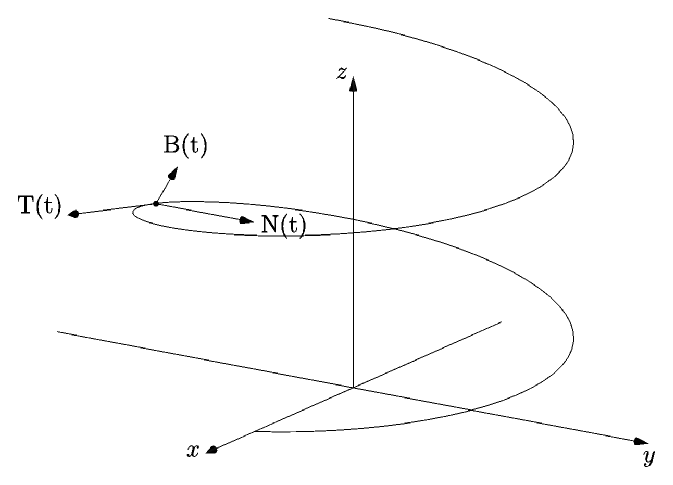
\includegraphics[width=12cm]{figure22.eps}
\caption{The tangent, normal and binormal to a helix in
$\RR^3$}
\label{figure-three-unit-vectors}
\end{figure} 

Let's complete these definitions with interpretation.
We've already spent some time on the unit tangent vector
$T(t)$. It represents the direction of movement of the curve at
that point. The associated scalar is speed, measuring how fast
the object is moving at this point in the curve.
The normal vector $N(t)$ represents the direction of
curvature. Curvature was a scalar, measuring how curved the
curve is at this point. The normal vector adds to this scalar a
direction, telling you which way the curve is turning. The two
vectors $T$ and $N$ determine a plane. 

\begin{defn}
The plane determined by $T$ and $N$is called the
\emph{osculating plane}. 
\end{defn}
If a parametric curve isn't twisted, the osculating plane is
the plane on which the curve travels.  The binormal vector
$B(t)$ is perpendicular to the osculating plane. Since planes
are best described by their normals, we use $B(t)$ to keep
track of the osculating plane.

Our third type of movement was twisting movement, where we
allowed a curve path to twist away from its plane of movement.
Since the osculating plane is determined by its normal $B(t)$,
twisting motion involves the change in $B(t)$. 

\begin{defn}
Let $\gamma(s): [0,L] \rightarrow \RR^3$ be a parametric curve
parametrized by arclength. Its \emph{torsion} is written
$\tau(s)$ and defined by the formula
\begin{equation*}
\tau(s) = \left| \frac{d B(s)}{ds} \right|.
\end{equation*}
\end{defn}

Torsion is a scalar that measures the change in $B$, the change
in the normal of the osculating plane. It meausre the rate of
twisting, the tendency of curving paths to change their plane
of motion.

As with curvature, we want to calculate torsion in an
arbitrary parametrization.

\begin{prop}
Let $\gamma(t): [a,b] \rightarrow \RR$ be a parametric curve in
an arbitrary parametrization. Then its torsion is calculabed
by the formula
\begin{equation*}
\tau(t) = \frac{-1}{|\gamma^\prime(t)|} B^\prime(t) \cdot
N(t).
\end{equation*}
\end{prop}

\begin{proof}
The arclength parameter is related to the parameter $t$ by the
arlencth function $s = s(t)$. The chain rule calculates the
derivative of the binormal vector.
\begin{equation*}
\frac{dB(t)}{dt} = \frac{dB(t(s))}{ds} \frac{ds}{dt} 
\end{equation*}
We can rearrange this expression.
\begin{equation*}
\frac{dB(s)}{ds} = \frac{\frac{dB(t)}{dt}}{\frac{dt}{ds}}
= \frac{B^\prime(t)}{|\gamma^\prime(t)|}
\end{equation*}
Without proof, $B^\prime(t)$ points in the direction of the
negative of the normal, $-N(t)$. To get the torsion, which is
the length of the vector in the previous formula, we can take
the dot product with the unit vector in this direction, which
is simply $-N(t)$.
\end{proof}

Now we have three scalars (speed, curvature, torsion) and
three matching vectors (tangent, normal and binormal).
Together, this information completely describes motion in
$\RR^3$. For convenience, the next list collects the
definitions of all six of these mathematical objects.
\begin{align*}
\gamma(t) & = (x(t), y(t), z(y))\\
\gamma^\prime(t) & = (x^\prime(t), y^\prime(t), z^\prime(t))\\
v(t) = |\gamma^\prime(t)| & = \sqrt{x^\prime(t)^2 + y^\prime(t)^2
+ z^\prime(t)^2 } \\
T(t) & = \frac{\gamma^\prime(t)}{|\gamma^\prime(t)|} \\
\kappa(t) & = \frac{|T^\prime(t)|}{|\gamma^\prime(t)|} \\
N(t) & = \frac{ T^\prime(t)}{|T^\prime(t)|} \\
B(t) & = T(t) \times N(t) \\
\tau(t) & = - \frac{B^\prime(t)}{|\gamma^\prime(t)|} \cdot N(t)
\end{align*}

\begin{example} 
Let $r$ and $h$ be two positive scalars. Consider the helix
$\gamma(t) = (r\cos t, r\sin t, ht)$. In the helix, $r$ is the
radius of the circular movement of the helix, and $h$ is the
rate of linear movement along the axis of the helix. Let's
calculate all the information about the motion along the
helix: the speed ($v$), curvature
($\kappa$), torsion ($\tau$),the tangent, the normal and
finally the binormal.
\begin{align*}
\gamma^\prime(t) & = (-r \sin t, r \cos t, h) \\
v = |\gamma^\prime(t)| & = \sqrt{r^2 \sin^2 t + r^2 \cos^2 t + h^2}
= \sqrt{r^2 + h^2} \\
T(t) & = \frac{\gamma^\prime(t)}{|\gamma^\prime(t)|} =
\frac{1}{\sqrt{r^2+h^2}} (-r \sin t, r \cos t, h) \\
T^\prime(t) & = \frac{1}{\sqrt{r^2 + h^2}} ( -r \cos t, -r \sin t,
0) \\
|T^\prime(t)| & = \frac{1}{\sqrt{r^2 + h^2}} \sqrt{r^2 \cos^2 t +
r^2 \sin^2 t} = \frac{r}{\sqrt{r^2 + h^2}} \\
\kappa(t) & = \frac{|T^\prime(t)|}{|\gamma^\prime(t)|} =
\frac{\frac{r}{\sqrt{r^2 + h^2}}}{\sqrt{r^2 + h^2}} =
\frac{r}{r^2 + h^2} \\
N(t) & = \frac{ T^\prime(t)}{|T^\prime(t)|} =
\frac{1}{\sqrt{r^2+h^2}}{r}{\sqrt{r^2 + h^2}} (-r\cos t, -r \sin
t, 0) \\
& \quad \quad = \frac{1}{r} (-r \cos t, -r \sin t, 0) = (-\cos t, -\sin
t, 0) \\
B(t) & = T(t) \times N(t) = \frac{1}{\sqrt{r^2 + h^2}} (-r \sin
t, r \cos t, h) \times (-\cos t, - \sin t, 0) \\
& \quad \quad = \frac{1}{\sqrt{r^2 +
h^2}} (h \sin t, -h \cos t, r) 
\end{align*}

\begin{align*}
B^\prime(t) & = \frac{1}{\sqrt{r^2 + h^2}} (h \cos t, h \sin t,
0) \\
\tau(t) & = - \frac{B^\prime(t)}{|\gamma^\prime(t)|} \cdot N(t)
= \frac{1}{r^2 + h^2} (h \cos t, h \sin t , 0 ) \cdot (-\cos t,
- \sin t, 0) = \frac{h}{r^2 + h^2}
\end{align*}
Look at the three scalars. 
\begin{equation*}
v = \sqrt{r^2 + h^2} \hspace{1.5cm}
\kappa = \frac{r}{r^2 + h^2} \hspace{1.5cm} 
\tau = \frac{h}{r^2 + h^2} \hspace{1.5cm} 
\end{equation*}
All three, speed, curvature and torsion, are constant here.
Let's summarize what kind of shapes of curves we get for
constant and zero values of the three scalars describing the
motion of parametric curves. 
\begin{tabular}{llll}
$v = 0$ & $\kappa = 0$ & $\tau = 0$ & $\implies$ no movement
at all \\
$v = c$ & $\kappa = 0$ & $\tau = 0$ & $\implies$ straight line
movement, no curving or twisting \\
$v = c_1$ & $\kappa = c_2$ & $\tau = 0$ & $\implies$ tracing
around a circle, constant speed and curvature, no twisting \\
$v = c_1$ & $\kappa = c_2$ & $\tau = c_3$ & $\implies$ helix,
constantly moving, curving and twisting
\end{tabular}

Like the straight line and the circle, the helix is the unique
curve which has constant non-zero speed, torsion and
cruvature. 
\end{example}

\section{Acceleration and Movement in Space}
\label{acceleration}

Now that we understand how parametric curves describe motion
in $\RR^3$, we can do some physics. This section tries to
undertstand what acceleration means in the language of
parametric curves. The starting point is simple: acceleration
should be the second derivative of the curve. 
\begin{equation*}
a(t) = \gamma^{\prime \prime}(t) = \frac{d}{dt}
\gamma^\prime(t) 
\end{equation*}
This means acceleration is a vector. Let's work out its
direction and magnitude, using $T$, $N$ and $B$ as reference
for direction. Recall the definition of the unit tangent.
\begin{equation*}
T(t) = \frac{\gamma^\prime(t)}{|\gamma^\prime(t)|} 
\end{equation*}
We solve for $\gamma^\prime(t)$.
\begin{equation*}
\gamma^\prime(t) = \underbrace{|\gamma^\prime|}_{\text{scalar}} 
\cdot \underbrace{T(t)}_{\text{direction}} 
\end{equation*}
We differentiate this, using the product rule.
\begin{equation}
\label{equation-reference2}
\frac{d}{dt} \gamma^\prime(t) = \left( \frac{d}{dt}
|\gamma^\prime(t)| \right) T(t) + |\gamma^\prime(t)|
\frac{d}{dt} T(t) 
\end{equation}
Recall the definition of the normal.
\begin{equation*}
N(t) = \frac{T^\prime(t)}{|T^\prime(t)|} 
\end{equation*}
We isolate $T^\prime(t)$.
\begin{equation}
\label{equation-reference1}
T^\prime(t) = |T^\prime(t)| N(t) 
\end{equation}
Finally, recall the definition of curvature.
\begin{equation*}
\kappa(t) = \frac{|T^\prime(t)|}{|\gamma^\prime(t)|}
\implies |T^\prime(t)| = \kappa(t) |\gamma^\prime(t)|
\end{equation*}
We use this expression to replace $|T^\prime(t)|$ in Equation
\ref{equation-reference1}.
\begin{equation*}
T^\prime(t) = \kappa(t) |\gamma^\prime(t)| N(t)
\end{equation*}
We put this expression for $T^\prime(t)$ into the second term
of Equation \ref{equation-reference2}, then group and label the
terms.
\begin{equation*}
a(t) = \underbrace{\frac{d}{dt}
|\gamma^\prime(t)|}_{\text{linear acceleration}} T(t) +
\underbrace{\kappa(t) |\gamma^\prime(t)|^2}_{\text{angular
acceleration}} N(t) 
\end{equation*}

\begin{defn}
Let $\gamma(t): [a,b] \rightarrow \RR^3$ be a parametric
curve. Its \emph{linear acceleration} is the vector
$\frac{d}{dt} |\gamma^\prime(t)| T(t)$ and its \emph{angular
acceleration} is the vector $\kappa(t) |\gamma^\prime(t)|^2
N(t)$. Linear acceleration tells us how quickly the speed changes.
Angular acceleration tells us how quickly the direction
changes. 
\end{defn}

\begin{example}
For the helix, $|\gamma^\prime(t)|$ is constant, so the
acceleration is entirely angular.
\begin{equation*}
a(t) = 0 T(t) + r N(t) = r N(t)
\end{equation*}
This makes sense, since the linear speed doesn't every change;
only the direction changes as the helix curves and twists. 
\end{example}

\section{Conics}
\label{conics}

We are going to need conics to talk about orbital mechanics in
the next section. Let's first review the classical definitions
of the four types of conics.

\begin{defn}
The \emph{circle} is all points equidistant from a center point
(focus). It is determined entirely by its
centre point and radius.
\begin{align*}
\text{Parameters} \hspace{2cm} & \text{Radius } r \vspace{0.3cm} \\
\text{Equation at } (0,0) \hspace{2cm} & x^2 + y^2 = r^2
\vspace{0.3cm} \\
\text{Equation at } (x_0, y_0) \hspace{2cm} & (x-x_0)^2 +
(y-y_0)^2 = r^2 \vspace{0.3cm} \\
\end{align*}
\end{defn}

\begin{defn}
The \emph{ellipse} is all points equidistant from $\emph{two}$ points
(foci). For the ellipse centered at the origin, the foci are
$(\pm c,0)$ where $c^2 = a^2 - b^2$. The ellipse is
determined by a centre point and two axis length, or by the
two foci and a distance. (This description of the ellipse
assumes $a > b$. If $a < b$, the semimajor and semiminor axes
are switched, since the major axis is always larger, the foci
would be on the $y$ axis instead of the $x$, axis and $c^2 =
b^2 - a^2$.) 
\begin{align*}
\text{Parameters} \hspace{2cm} & \text{Semimajor axis } a \ \ 
\text{Semimnior axis } b \vspace{0.3cm} \\
\text{Equation at } (0,0) \hspace{2cm} & \frac{x^2}{a^2} +
\frac{y^2}{b^2} = 1 \vspace{0.3cm} \\
\text{Equation at } (x_0, y_0) \hspace{2cm} &
\frac{(x-x_0)^2}{a^2} + \frac{(y-y_0)^2}{b^2} = 1
\vspace{0.3cm} \\
\end{align*}
\end{defn}

\begin{defn}
The \emph{parabola} is all points which are equidistant to a point
(focus) and a line (directrix). For the parabola centered at the
origin, the focus is $(0,p)$ and the directrix is the line $y = -p$.
The focus and directrix entirely determine the parabola.
(This description holds for upward opening parabolae. If the
directrix is $y = p$ and the focus $(0, -p)$, then $x^2 = -4py$ is
the downward facing parabola. Switching the roles of $x$ and $y$
gives left or right facing parabolae.)
\begin{align*}
\text{Parameters} \hspace{2cm} & \text{Focus - Directrix
Distance } 2p \vspace{0.3cm} \\
\text{Equation at } (0,0) \hspace{2cm} & x^2 = 4py
\vspace{0.3cm} \\
\text{Equation at } (x_0, y_0) \hspace{2cm} & (x-x_0)^2 =
4p(y-y_0) \vspace{0.3cm} \\
\end{align*}
\end{defn}

\begin{defn}
The \emph{hyperbola} is all points where the \emph{difference}
of the distances to the two foci is constant. The foci,
similar to the ellipse, are the points $(\pm c,0)$ with $c^2 =
a^2 + b^2$. The hyperbola has vertices $(\pm a,0)$, which are
the points closest to the origin.  In addition, it has
asymptotes, which are the lines $y = \pm \frac{b}{a} x$. The
hyperbola is determined by its two foci and a distance. (This
description is for hyperbolae which open along the $x$ axis.
Switching $x$ and $y$ gives hyperbolae which open along the
$y$ axis.)
\begin{align*}
\text{Parameters} \hspace{2cm} & \text{Axes } a, \ b
\vspace{0.3cm} \\
\text{Equation at } (0,0) \hspace{2cm} & \frac{x^2}{a^2} -
\frac{y^2}{b^2} = 1 \vspace{0.3cm} \\
\text{Equation at } (x_0, y_0) \hspace{2cm} &
\frac{(x-x_0)^2}{a^2} - \frac{(y-y_0)^2}{b^2} = 1 \vspace{0.3cm} \\
\end{align*}
\end{defn}

\subsection{Eccentricity}
\label{eccentricity}

The parabola is defined as all points equidistant from a focus
and a directrix. All other conics have foci, but the parabola
is the only with a directrix. However, there is another method
of describing all conics in terms of focus and directrix.  To
get to that description, consider first the parabola in more
detail in the following diagram. In Figure
\ref{figure-focus-directrix}, we've labeled the conic
itself as $\gamma$, the focus $F$ and the directrix $L$ and
the distance between the focus and the directrix, labeled $d$.

\begin{figure}[t]
\centering
\includegraphics[width=12cm]{figure23.eps}
\caption{Conic definition with directrix $L$ and focus $F$}
\label{figure-focus-directrix}
\end{figure} 

We've also labeled an angle $\theta$ and two distances $r$ and
$l$ in this diagram. The point $P$ is, by definition, on the
parabola because the distances from $P$ to the focus and to
the directrix are equal.  In Figure \ref{figure-focus-directrix},
$r=l$.

We can generalize the construction  by allowing $r$ and $l$ to
be non-equal, but insisting that their ration is constant.
That is, given a focus $F$ and a directrix $L$, we consider
all points $P$, such $\frac{r}{l}$ is a constant. $\frac{r}{l}
= 1$ will recover the parabola, but other choices of the
constant will result, amazingly, in other conics. 

\begin{defn}
The \emph{eccentricity} of a conic defined via a focus and
a directix is the ratio $\frac{r}{l}$ of the distance to the
focus over the distance to the directrix.
\begin{equation*}
e = \frac{r}{l}
\end{equation*}
\end{defn}

We would like to get a description of conics as a
parametric curves using the focus, directrix and eccentricity. We
will use polar coordinates for this, assuming that $F$ is at
the origin. In Figure \ref{figure-focus-directrix}, putting $F$
at the origin means that $r$ and $\theta$, as labelled, are
exactly polar coordinates. 

\begin{prop}
Let $\gamma$ be a conic described by a focus at the origin, a
directrix $x=d$ and an eccentricity $e$. Then $\gamma$ is
described by a polar locus,
\begin{equation*}
r = \frac{ed}{1 + e \cos \theta},
\end{equation*}
or by a polar parametric curve using $\theta$ as the
parameter,
\begin{equation*}
\gamma(\theta) = (r(\theta), \theta) = \left(\frac{ed}{1 + e
\cos \theta}, \theta\right)
\end{equation*}
\end{prop}

\begin{proof}
From the diagram and some trigonometry, we can see that $l = d
- r\cos \theta$. Eccentricity is the ratio of $r$ to $l$, so
eccentricity has this form:
\begin{equation*}
e = \frac{r}{d-r\cos\theta}
\end{equation*}
If we solve for $r$ in this equaiton we get the desired polar
locus.
\begin{equation}
\label{equation-conic-eccentricity-form}
r = \frac{ed}{1 + e \cos \theta}
\end{equation}
Then we simply choose $\theta$ as the parameter for the
polar parametric description.
\end{proof}

\begin{prop}
\label{prop-conic-eccentricity}
All four conics can be defined in terms of a focus $F$,
directrix $L$, and eccentricity $e$. A conic is thus redefined
to be all points where the ratio of the distance to the focus
over the distance to the directrix is constant and equal to
the eccentricity. The hyperbola has eccentricity $e>1$, the
parabola has eccentricity $e=1$, the ellipse has eccentricity
$e<1$. The circle is the special limit case $e=0$, though to
realize the shape we have to allow the distance between $F$
and $L$ to approach infinity.
\end{prop}

\begin{proof}
We will prove all cases except the limit case of the circle.
Our approach is to start with the polar locus and try to
recover the standard equations of the conics from the start of
this section.

We start with the polar locus and change back to Cartesian
coordinates, using the change of coordinates equations: $r =
\sqrt{x^2 + y^2}$ and $r \cos \theta = x$.
\begin{align*}
\frac{r}{d - r\cos \theta} & = e \\
\frac{\sqrt{x^2 + y^2}}{d - x} & = e \\
\sqrt{x^2 + y^2} & = ed -ex = e(d-x) \\
x^2 + y^2 & = e^2 (d^2 - 2dx + x^2) 
\end{align*}
We rearrange this to get a polynomial expression in $x$.
\begin{equation}
\label{equation-reference3}
(1-e^2)x^2 + 2de^2 x + y^2 = d^2 e^2 
\end{equation}
If $e \neq 1$, we divide through by $(1-e^2)$, then proceed to
complete the square in the $x$ term.
\begin{align*}
x^2 + \frac{2de^2}{1-e^2} x + \frac{y^2}{1-e^2} & = \frac{d^2
e^2}{1-e^2} \\
x^2 + \frac{2de^2}{1-e^2} x + \frac{d^2e^4}{(1-e^2)^2} -
\frac{d^2e^4}{(1-e^2)^2} + \frac{y^2}{1-e^2} & = \frac{d^2
e^2}{1-e^2} \\
\left( x + \frac{e^2d}{1-e^2} \right)^2 + \frac{y^2}{1-e^2} &
= \frac{d^2 e^2}{1-e^2} + \frac{d^2e^4}{(1-e^2)^2}
\intertext{We take the right-hand side to common denominator.}
\left( x + \frac{e^2d}{1-e^2} \right)^2 + \frac{y^2}{1-e^2} & 
= \frac{d^2 e^2(1-e^2) + d^2e^4}{(1-e^2)^2} \\
\left( x + \frac{e^2d}{1-e^2} \right)^2 + \frac{y^2}{1-e^2} & 
= \frac{d^2 e^2}{(1-e^2)^2} \\
\intertext{We divide by the right-hand side.}
\frac{\left( x + \frac{e^2d}{1-e^2}
\right)^2}{\frac{d^2e^2}{(1-e^2)^2}} +
\frac{\frac{y^2}{1-e^2}}{\frac{d^2e^2}{(1-e^2)^2}} & = 1 \\
\frac{\left( x + \frac{e^2d}{1-e^2}
\right)^2}{\frac{d^2e^2}{(1-e^2)^2}} +
\frac{y^2}{\frac{d^2e^2}{1-e^2}} & = 1
\intertext{The sign in from of the $y^2$ term is positive if
$1-e^2 > 1$, that is, when $e<1$. Otherwise, $e^2-1$ is
positive. In the positive case, we can rewrite the expression
as a difference of squares.}
\frac{\left( x + \frac{e^2d}{1-e^2}
\right)^2}{\frac{d^2e^2}{(1-e^2)^2}} -
\frac{y^2}{\frac{d^2e^2}{e^2-1}} & = 1
\end{align*}
In the case $e<1$, the expression is the sum of positive
squares, so we have an ellipse. In the case $e>1$,
the expression is the difference of positive square, so we
have a hyperbola. For future convenience, we define the
following constants for the $e<1$ (ellipse) case.
\begin{equation}
\label{equation-reference7}
x_0 = \frac{-e^2 d}{1-e^2} \quad \quad 
a^2 = \frac{e^2 d^2}{(1-e^2)^2} \quad \quad 
b^2 = \frac{e^2 d^2}{1-e^2} \quad \quad 
\end{equation}
Subsituting these cosntant into the previous equation gives an
elegant ellipse equation.
\begin{equation*}
\frac{(x-x_0)^2}{a^2} \pm \frac{y^2}{b^2} = 1
\end{equation*}

Lastly, in Equation \ref{equation-reference3} we excluded $e = 1$. Now
assume $e=1$, which removes the $(1-e^2)x^2$ term from
Equation \ref{equation-reference3} entirely. We continue the
derivation from that point; the calculation is much easier in
this case. 
\begin{equation*}
2dx + y^2 = d^2 \implies
y^2 = d^2 - 2dx \implies
y^2 = -2d \left( x - \frac{d}{2} \right)
\end{equation*}
This is the equation for a leftward-opening parabola, so $e=1$
does recover the parabola. 

For all cases except the circle, we recovered the standard
equation of the conic. We found a hyperbola when $e>1$, an
ellipse when $e<1$, and a parabola when $e=1$. As mentioned in
the proposition, the circle is a strange limit case as $e
\rightarrow 0$, but $e \rightarrow 0$ also increases the
distance $d \rightarrow \infty$. 
\end{proof}

\section{Kepler's Laws}
\label{kepler}

\begin{figure}[t]
\centering
\includegraphics[width=12cm]{figure24.eps}
\caption{An orbital path for Kepler's laws}
\label{figure-keplers-laws}
\end{figure} 

Kepler's laws were originally formulated from the observations
of planets in the night sky and were written down before
Newton. One of the triumphs of Newtonian mechanics is the
recovery of Kepler's laws. In this section, we start with
Newton's gravity and derive Kepler's laws.

Kepler described three laws of planetary motion. 
\begin{itemize}
\item Satellites in orbit around a large gravity source have
elliptical orbits with the large object at one of the foci of
the ellipse.
\item The radius of a satellite sweeps out equal area over time.
\item The period $T$ of a satellite and the major axis $a$ of the
associated ellipse satisfy $T^2 = \alpha a^3$ for some
constant $\alpha$ depending only upon the mass of the large object.
\end{itemize}

\subsection{Kepler's First Law}
\label{kepler-first}

The setup for approaching Kepler's laws is show in Figure
\ref{figure-keplers-laws}.
\begin{itemize}
\item We have a large stationary object of mass $M$, and a small
object of mass $m$ in orbit around the larger object. We must
assume that $m \ll M$ to allow the larger object to be
essentially stationary.
\item We place the stationary object of mass $M$ at the origin
in $\RR^3$. We might work in the plane since the orbits are
planar, but it is more useful to think of the orbit sitting in
the $xy$ plane in $\RR^3$. This will be important, since it
turns out to be useful to consider the perperdicular direction
to the plane of orbit and use normals and binormals in
$\RR^3$. 
\item The curve $\gamma(t) = (r(t),\theta(t),z(t))$ decribes the
motion of the orbiting object over time, in cylindrical
coordinates (which reduce to polar coordinates in the $xy$
plane). In the third coordinate $z(t)$, we expect
that $z(t) = 0$ at all times $t$ (which will produce a curve
in the $xy$ plane in polar coordinates), but we don't assume
this. 
\item The curve $\gamma(t)$ is unknown and we wish to derive it
from Newtonian physics. We will prove Kelper's laws using the
derived curve.
\item The force of gravity has magnitude
\begin{equation*}
F = \frac{GmM}{|\gamma(t)|^2} = \frac{GmM}{r(t)^2}.
\end{equation*}
\item The direction of the force is $-\gamma(t)$, since the
force wishes to pull the object back towards the origin. Since
we want just direction without changing magnitude, we use the
unit vector $u(t) = \gamma(t) / |\gamma(t)|$ for the direction
of $\gamma(t)$. 
\item Newton's first law $F = ma$ applies, so the acceleration
is 
\begin{equation*}
a(t) = \frac{-GM}{|\gamma(t)|^2} u(t) =
\frac{-GM}{|\gamma(t)|^3} \gamma(t).
\end{equation*}
\item Acceleration is the second derivative of position,
therefore Newton's first law becomes
\begin{equation*}
\frac{d^2}{dt^2} \gamma(t) = \frac{-GM}{|\gamma(t)|^3}
\gamma(t)
\end{equation*}
\item We write $h(t) = \gamma(t) \times \gamma^\prime(t)$.
$h(t)$ is in the binormal direction, but is not necessarily a
unit vector. This seems like a strange definition, but the
vector $h$ turns out to be very useful in the proof. 
\end{itemize}

Newton's law is a multivariable differential equation; solving
it directly is very difficult and well beyond the scope of
this course. Our approach is indirect. We start with two
seeminly random calculations. For convenience of notation, we
often drop the $t$ variable, writing $\gamma$ instead of
$\gamma(t)$ and likewise for other functions of $t$.

\begin{lem}
\label{lemma-reference1}
\begin{equation*}
\frac{d}{dt} h(t) = 0
\end{equation*}
\end{lem}

\begin{proof}
\begin{equation*}
\frac{d}{dt} h(t) = \frac{d}{dt} \gamma \times \gamma^\prime =
\frac{d\gamma}{dt} \times \gamma^\prime + \gamma \times
\frac{d\gamma^\prime}{dt} 
= \gamma^\prime \times \gamma^\prime + \gamma \times a 
\end{equation*}
The first term $\gamma^\prime \times \gamma^\prime = 0$ since
any vector with itself in the cross product is $0$. Then
$\gamma$ and the acceleration $a$ are in the same direction
(up to $\pm1$), since the force pulls back towards the origin.
Vectors in the same direction likewise have $0$ cross product.
Therefore, we have $\frac{d}{dt} h = 0$. 
\end{proof}

\begin{lem}
\label{lemma-reference2}
\begin{equation*}
h = |\gamma|^2 (u \times u^\prime)
\end{equation*}
\end{lem}

\begin{proof}
We can write $h$ this way.
\begin{align*}
h(t) & = \gamma \times \gamma^\prime =
(|\gamma|u) \times \frac{d}{dt} (|\gamma| u) \\
\intertext{We use the product rule on the second term.}
& = |\gamma| u \times \left( u \frac{d}{dt} |\gamma| + |\gamma|
\frac{d}{dt} u \right) 
= |\gamma| u \times u \frac{d}{dt} |\gamma| + |\gamma| u
\times |\gamma| \frac{d}{dt} u \\
& = |\gamma| \frac{d}{dt} |\gamma| (u \times u ) + |\gamma|^2
u \times u^\prime \\
h & = |\gamma|^2 (u \times u^\prime) 
\end{align*}
\end{proof}

\begin{prop}
(Kepler's First Law) The differential equation 
\begin{equation*}
a = \frac{-GM}{|\gamma|^2} u 
\end{equation*}
can be solved with a polar parametric curve $\gamma(t) =
(r(t),\theta(r))$ which satisfies the equation
\begin{equation*}
r(t) = \frac{ed}{1 - e \cos \theta(t)}.
\end{equation*}
This is exactly the same as Equation
\ref{equation-conic-eccentricity-form}. By Proposition
\ref{prop-conic-eccentricity} such forms describe all conics, so
Kepler's First Law states that orbital paths are conics. 
\end{prop}

\begin{proof}
We start with Newton's First Law as a differential equation,
using the force of gravity on the right side. 
\begin{equation*}
a = \frac{-GM}{|\gamma|^2} u 
\end{equation*}
Let's take the cross product with $h$. We use Lemma
\ref{lemma-reference2} on the right side.
\begin{align*}
a \times h & = \frac{-GM}{|\gamma|^2} u \times h 
= \frac{-GM}{|\gamma|^2} u \times \left( |\gamma|^2
(u \times u^\prime) \right) \\
& = \frac{-GM}{|\gamma|^2} |\gamma|^2 \left( u \times \left( u
\times u^\prime \right) \right) = -GM \left( u \times \left( u \times
u^\prime \right) \right) \\
\intertext{We use Proposition \ref{prop-triple-cross-product} to
expand the triple cross product on the right side.}
a \times h & = -GM ((u\cdot u^\prime) u - (u \cdot u) u^\prime)) 
\end{align*}
Since $u$ is always a unit vector, we can apply
Lemma \ref{lemma-unit-vector-derivative}, which says that 
$u \times u^\prime = 0$. Also since $u$ is a unit vector, $u
\cdot u = |u|^2 = 1$. This deals with both of the dot
products.
\begin{equation}
\label{equation-reference4}
a \times h = -GM ( 0 u - 1 u^\prime) = GM u^\prime
\end{equation}

Then we consider the following derivative.
\begin{equation*}
\frac{d}{dt} (\gamma^\prime \times h) =
\frac{d\gamma^\prime}{dt} \times h + \gamma^\prime \times
\frac{dh}{dt} 
\end{equation*}
The first term here is $a \times h$, since $a$ is
$\frac{d\gamma^\prime}{dt}$. The second term involves the
derivative of $h$. But Lemma \ref{lemma-reference1} said that the
derivative of $h$ is zero, so this term vanishes.
\begin{equation*}
\frac{d}{dt} (\gamma^\prime \times h) = a \times h
\end{equation*}
Then let's replace $a \times h$ with the expression from
Equation \ref{equation-reference4}. 
\begin{equation*}
\frac{d}{dt} (\gamma^\prime \times h) = GM u^\prime
\end{equation*}
Now we've made progress with our difficult differential
equation: we have a time derivative on both sides. We can
simply integrate both sides to give $\gamma^\prime \times h =
GM u + c$. where $c$ is a \emph{vector} of constants of
integration. (That vector corresponds to intial conditions of
position and velocity). We take the dot product with
$\gamma$.
\begin{equation*}
\gamma \cdot (\gamma^\prime \times h) = GM (u \cdot \gamma) +
\gamma \cdot c = GM |\gamma| u \cdot u + |\gamma| |c| \cos
\theta = GM + |\gamma| |c| \cos \theta
\end{equation*}
Here $\theta$ is the angle between $\gamma$ and $c$. Since we
haven't specified a starting point, we can choose coordinates
such that $c$ is in the positive $x$ direction, which means that
this $\theta$ is the usual $\theta$ of polar coordinates and
$|\gamma|$ is the usual $r$ of polar coodinates. 
\begin{align*}
\gamma \cdot (\gamma^\prime \times h) & = GM |\gamma| +
|\gamma| |c| \cos \theta \\
\intertext{We solve for $|\gamma|$.}
|\gamma| & = \frac{\gamma \cdot (\gamma^\prime \times h) } {
GM + |c| \cos \theta}
\end{align*}
The expression $|c|/GM$ is a constant, so let's give it a
label. 
\begin{equation}
\label{equation-reference8}
e \defeq \frac{|c|}{GM}
\end{equation}
Let's switch the $|\gamma|$ for $r$ as well. 
\begin{equation*}
r = \frac{\gamma \cdot (\gamma^\prime \times h) } { GM + |c| \cos
\theta} = \frac{\gamma \cdot (\gamma^\prime \times h) } { 1 + e \cos
\theta} \left( \frac{1}{GM} \right) 
\end{equation*}
The numerator involves $\gamma \cdot (\gamma^\prime \times
h)$, which we can rearrange to $h \cdot (\gamma \times
\gamma^\prime)$ using Proposition \ref{prop-cross-dot-product}. But
$(\gamma \times \gamma^\prime)$ is the definition of $h$, so
this dot product is $h\cdot h = |h|^2$. 
\begin{equation}
\label{equation-reference10}
r = \frac{|h|^2 } { 1 + e \cos
\theta} \left( \frac{1}{GM} \right) 
\end{equation}
$|h|^2$ is a constant, since $h$ doesn't change according to
Lemma \ref{lemma-reference1}. Let's make another definition.
\begin{equation}
\label{equation-reference9}
d = |h|^2/|c|
\end{equation}
We can then replace the nuemrator of Equation
\ref{equation-reference10} using $d$. 
\begin{equation*}
r = \frac{d|c|} { 1 + e \cos
\theta} \left( \frac{1}{GM} \right) 
= \frac{d} { 1 + e \cos
\theta} \left( \frac{|c|}{GM} \right) 
\end{equation*}
Replace $\frac{|c|}{GM}$ by $e$, since that's how we defined
$e$ in Equation \ref{equation-reference8}.
\begin{equation*}
r = \frac{ed } { 1 + e \cos \theta} 
\end{equation*}
This is the desired form.
\end{proof}

The eccentricity was defined as $e = |c|/GM$.  Notice that the
eccentricity depends on the constants of integration. That
makes sense since those constants determine inital position
and velocity.  If $e<1$, then the initial conditions indicate
an ellipse. If $e \geq1$ then we get a hyperbola. The
difference is precisely the notion of escape velocity -- these
initial conditions tell us if the satellite has enough initial
energy to escape or be trapped in orbit. If trapped in orbit,
the orbits are elliptical. If escaping, the path is parabolic
or hyperbolic. We will assume that the orbits are elliptical,
i.e., that the original velocity is less than escape velocity,
to prove the final two laws.

\subsection{Kepler's Second Law}
\label{kepler-second}

\begin{prop}
(Kepler's Second Law). The area swept out by a line
between the M and the satellite is constant in time.
\end{prop}

\begin{figure}[ht]
\centering
\includegraphics[width=12cm]{figure25.eps}
\caption{Approximate movement along the orbit over time
$dt$.}
\label{figure-sweeping-area}
\end{figure} 

\begin{proof}
Write $A(t)$ for the area swept out in this way. Our goal is
to prove that $A^\prime(t)$ is constant. We approach this by
looking at the infinitesimal area $dA$ swept out over an
infinitesimal time interval $dt$. Such an area is a small
triangle, shown in gray in Figure \ref{figure-sweeping-area}. It has
side length $r$ and base $db$, which we can assume is
perpendicular to the radius.  Therefore, the area $dA$ of the
infinitesimal triangle is $\frac{1}{2} r db$. Then $db$, as an
infinitesimal arclength, is $rd\theta$, so $dA = \frac{1}{2}
r^2 d\theta$, which we can integrate (with a temporary
internal variable for the integration).
\begin{equation*}
A(t) = \int_0^t \frac{1}{2} r(w)^2 d\theta = \int_0^t \frac{1}{2}
r(w)^2 \frac{d\theta}{dw} dw 
\end{equation*}
We calculate the derivative $\frac{dA}{dt}$.
\begin{equation*}
\frac{dA}{dt} = \frac{d}{dt} \int_0^t \frac{1}{2} r(w)^2
\frac{d\theta}{dw} dw = \frac{1}{2} r(t)^2 \frac{d\theta}{dt}
\end{equation*}
Now we return to some of the derivations of the previous section
to understand this equation. Recall $r(t) = |\gamma(t)|$. In
Cartesian coordinates, $\gamma$ has this form.
\begin{equation*}
\gamma(t) = (r(t) \cos \theta(t), r(t) \sin \theta(t), 0) 
\end{equation*}
The the unit vector $u = \gamma(t) / |\gamma(t)|$ is $u(t) =
(\cos \theta (t), \sin \theta(t),0)$. We calculate its
derivative.
\begin{equation}
\label{equation-reference6}
\frac{du}{dt} = (-\sin \theta(t), \cos \theta(t), 0)
\frac{d\theta}{dt} 
\end{equation}
We calculate $u \times u^\prime$.
\begin{equation}
\label{equation-reference5}
u \times \frac{du}{dt} = (\cos \theta(t), \sin \theta(t), 0)
\times (-\sin \theta(t), \cos \theta(t), 0) \frac{d\theta}{dt} =
(0,0,1) \frac{d\theta}{dt}
\end{equation}
Recall Lemma \ref{lemma-reference2}.
\begin{equation*}
h = |\gamma(t)|^2 u \times \frac{du}{dt} 
\end{equation*}
We replace the cross product on the right with the same
expression from Equation \ref{equation-reference5}.
\begin{equation*}
h = |\gamma(t)|^2 \frac{d\theta}{dt} (0,0,1)
\end{equation*}
We take the magnitude of this vector. (We choose a direction
of orbit for that $\frac{d\theta}{dt}$ is positive.)
\begin{equation*}
|h| = |\gamma(t)|^2 \frac{d\theta}{dt} = r(t)^2
\frac{d\theta}{dt}
\end{equation*}
Now this looks familiar: if has the same right side as Equation
\ref{equation-reference6}. Therefore, it is equation to the left side
of that equation.
$\frac{dA}{dt}$.
\begin{equation*}
\frac{dA}{dt} = \frac{1}{2} |h|
\end{equation*}
But we know that $h$ is constant by Lemma \ref{lemma-reference1}.
Therefore, the rate of change of the area $A$ must be
constant.
\end{proof} 

\subsection{Kepler's Third Law}
\label{kepler-third}

\begin{prop}
(Kepler's Third Law) The period $T$ of the revolution and the
semi-major axis $a$ of the ellipse satisfy $T^2 = \alpha a^3$
for some constant $\alpha$.
\end{prop}

\begin{proof}
We start with the last equation in the previous proof.
\begin{equation*}
A(t) = \frac{|h|}{2} t
\end{equation*}
The period $T$ is the time needed to complete one
whole orbit. The area swept out over time $T$ should be the
whole ellipse. Recall an ellipse with semiaxes $a$ and $b$ has
area $\pi a b$. We make the two areas equal.
\begin{equation}
\label{equation-reference11}
A(T) = \frac{|h|T}{2} = \pi a b \implies T = \frac{2\pi ab}{|h|}
\implies T^2 = \frac{4\pi^2 a^2 b^2}{|h|^2}
\end{equation}
From Equation \ref{equation-reference7}, we have expressions for the
semimajor and semiminor axes ($a$ and $b$) in terms of the
eccentricity $e$ and the distance $d$ from the focus to the
directrix. 
\begin{equation*}
a^2 = \frac{e^2 d^2}{(1-e^2)^2} \hspace{2cm} b^2 = \frac{e^2
d^2}{1-e^2}
\end{equation*}
We take the square root of $a^2$ and then the ratio of the
two equations.
\begin{equation}
\label{equation-reference12}
\frac{a}{b^2} =
\frac{\frac{ed}{(1-e^2)}}{\frac{e^2d^2}{1-e^2}} =
\frac{1}{ed} \implies ed = \frac{b^2}{a}
\end{equation}
Now we can relate $ed$ to $G$, $M$ and $h$. Recall the
definition of $e$ from Equation \ref{equation-reference8} and $d$
from Equation \ref{equation-reference10}. We calculate the product
$ed$. 
\begin{equation}
ed = \frac{|h|^2}{GM} \implies |h|^2 = edGM
\end{equation}
We use this to substitute for $|h|^2$ in 
\ref{equation-reference11}.
\begin{equation*}
T^2 = \frac{4\pi^2 a^2 b^2}{GMed} 
\end{equation*}
Then use Equation \ref{equation-reference12} to substitute for $ed$
and simplify. 
\begin{equation*}
T^2= \frac{4\pi^2 a^2 b^2}{\frac{GMb^2}{a}} = \frac{4\pi^2}{GM} a^3
\end{equation*}
This is the desired result. The proportionality constant is
$\frac{4\pi^2}{GM}$, which is certainly constant.
\end{proof}

\chapter{Topology of $\RR^n$}
\label{topology}

Topology is a branch of mathematics which studies concepts of
shape, near-ness and distance. You might think that such a
study woulds just be geometry, and you would be partially
correct. Topology is like a coarser version of geometry. It
cares about broad notions of near and far instead of precise
distances, and about types of shapes instead of precisely
defined specifics. Though it lacks the precision of other
parts of geometry, it is fundamental to modern mathematics.

We have already seen some topology of $\RR$ in single variable
calculus, mostly notably in the definition of open and closed
intervals: $(a,b)$ and $[a,b]$. Open intervals did not
include their endpoints but closed intervals did. Openness and
closedness are central to topolgoy. In this brief chapter, we
will extend the notions of opennes, closedness and intervals
to $\RR^n$. We will need these notions to understand
multivariable functions in the next section.

\section{Open and Closed Sets}
\label{open-closed}

\begin{defn}
Let $S$ be a set. A \emph{topology} on $S$ is a choice of
subsets which are open and which subsets are closed.
\end{defn}

We need two definitions to allow us to define open and
clsoed sets in $\RR^n$.

\begin{defn}
Let $A$ be a subset of $\RR^n$. A point $a \in A$ is called
an \emph{interior point} if there exists $\epsilon > 0$ such
that all points $b$ with $|a-b|< \epsilon$ are also in $A$.
\end{defn}

A point is an interior point if all nearby points are also in
the set. Around an interior point, we can move a little bit in
any direction and remain inside the set. This $\epsilon$
measures exactly how little the little bit of movement is.

\begin{defn}
Let $A$ be a subset of $\RR^n$. A point $a$ (not necessarily
in the set) is called a
\emph{boundary point} if for any $\epsilon > 0$ there exists
points $b_1$ and $b_2$ such that both $|b_i -
a|<\epsilon$, $b_1$ is in the set, but $b_2$ isn't. The
\emph{boundary} of a set is the set of all its boundary point.
\end{defn}

A point is a boundary point if there are nearby points in the
set and nearby points not in the set.  Nearby means within
some small distance, measured by the small positive number
$\epsilon$.  The two definitions are mutually exclusive: a
point cannot be both an interior and a boundary point for a
set. (It can, of course, be neither). These two definitions
allow us to define open and closed sets in $\RR^n$.

\begin{defn}
Let $A$ be a subset of $\RR^n$. Then $A$ is called
\emph{open} is all of its points are interior points.
Equivalently, $A$ does not contin any boundary points.
Alternatively, $A$ is called \emph{closed} if it contains
all of its boundary points (or, equivalently, if it contains
its boundary).
\end{defn} 

This definition properly extends the notions of open and
closed intervals in $\RR$. The boundary points 
of an interval are the endpoints. The open
intervals lacks their endpoints and the closed intervals
included their endpoints. In $\RR^n$, the boundaries are
much more complicated than endpoints: they can be intricate
geometric shapes. 

\begin{example}
The sphere $S^{n-1}$ in $\RR^n$ is all vectors of length one.
The closed ball $B^{n}$ in $\RR^n$ is all vectors of length
one or less. The sphere $S^{n-1}$is the boundary of the closed
ball $B^n$, and the closed ball is closed because all points
of the sphere are all contained in the closed ball. 
\end{example}

\section{Intervals}
\label{intervals}

In addition to open and closed sets in $\RR^n$, the is a
direct extension of intervals.

\begin{defn}
An \emph{open interval} in $\RR^n$ is a set of points $(x_1,
x_2, \ldots, x_n) \in \RR^n$ such that 
\begin{equation*}
a_1 < x_1 < b_1, \hspace{1cm} 
a_2 < x_2 < b_2, \hspace{1cm} \ldots \hspace{1cm} 
a_n < x_n < b_n 
\end{equation*}
It is written 
\begin{equation*}
I = (a_1,b_1)\times (a_2,b_2) \times \ldots \times (a_n,b_n).
\end{equation*}
\end{defn}

\begin{defn}
An \emph{closed interval} in $\RR^n$ is a set of points $(x_1,
x_2, \ldots, x_n) \in \RR^n$ such that 
\begin{equation*}
a_1 \leq x_1 \leq b_1, \hspace{1cm} 
a_2 \leq x_2 \leq b_2, \hspace{1cm} \ldots \hspace{1cm} 
a_n \leq x_n \leq b_n 
\end{equation*}
It is written 
\begin{equation*}
I = [a_1,b_1]\times [a_2,b_2] \times \ldots \times [a_n,b_n].
\end{equation*}
\end{defn}

Intervals are rectangular objects. In $\RR^2$, there are
filled-in rectangles, including the hollow bounding rectangle
if the interval is closed and excluding it if the interval is
open. In $\RR^3$, intervals are solid rectangular prisms
whose boundaries are rectangular boxes. In higher dimensions,
we think of intervals are higher-dimensional rectangular
prisms.

\chapter{Multivariable Functions and Partial Differentiation}
\label{multivariable-functions}

\section{Definitions}
\label{multivariable-functions-definitions}

First year calculus dealt with functions $\RR
\rightarrow \RR$. Parametric curves dealt with functions
$\RR \rightarrow \RR^n$. Multivariable functions are
functions $\RR^n \rightarrow \RR^m$. They having an arbitrary number
of inputs and outputs. We can distinguish between two main
categories, classified by output.

\begin{defn}
A \emph{scalar function} is a function $f: \RR^n \rightarrow
\RR$.
\end{defn}

\begin{defn}
A \emph{vector function} is a function $f: \RR^n \rightarrow
\RR^m$ for $m > 1$.
\end{defn}

Vector functions are the most difficult and complicated, since
they have both multiple inputs and multiple outputs. The study
of vector functions is the major topic of Calculus IV. For the
remainder of these notes, we will restrict our attention to
scalar functions.

\begin{example}
There are many familiar scalar functions. 
The potential energy due to gravity on an object with mass
$m$ and height $h$ above the surface of the earth is $PE = mgh$
is a two variable function.
In a circuit, voltage in terms of current and reisistance is $V
= IR$ is another two variable
function. The force of gravity between two celestial object
$F = -MmG/r^2$ is a three-variable functions which depends on
both masses, $M$ and $m$, as well as the distance between them
$r$. Any quantity which can vary in three dimensional space,
such a pressure, temperature, humidity, is a functions of the
three variables of location $(x,y,z)$.
\end{example} 

\begin{example}
\label{example-multivariable1}
Here are some explicit functions $\RR^2 \rightarrow \RR$. 
\begin{align*}
f_1(x,y) & = x-y \\
f_2(x,y) & = \sin (xy) \\
f_3(x,y) & = \frac{1}{2} x^y \\
f_4(x,y) & = x^2 + y^2 - xy \\
f_5(x,y) & = \sqrt{x} + \sqrt{y} \\
f_6(x,y) & = \sqrt{4 - x^2 -y^2}
\end{align*}
Any other algebraic expression in $x$ and $y$ would also
define a function $\RR^2 \rightarrow \RR$.
\end{example}

\begin{defn}
The \emph{domain} of a scalar function $f: \RR^n \rightarrow
\RR$ is the subset of $\RR^n$ where the function can be
defined. 
\end{defn}

Domain has the same kind of restrictions as for
single-variable functions: no division by zero, no negative
even roots, no negative logarithms, etc. However, now 
that the domain restrictions may apply to any of the input
variables. The domains themselves may be very complicated
subsets of $\RR^n$. 

\begin{example}
Let's look at the domains of the five explicitly stated
functions in the Example \ref{example-multivariable1}
\begin{smallitemize}
\item $f_1$ and $f_4$ are polynomials (in
two variables), so there are no restrictions. Their
domain is $\RR^2$. 
\item $f_2$ is a sine function, which again
imposes no restrictions, so it also has domain $\RR^2$.
\item $f_5$ has two square roots, one involving $x$ and one
involving $y$. Therefore, we need $x\geq 0$ and $y \geq 0$ to
defined $f_5$. That domain is the positive $x$ and $y$
quadrant, including the origin and the positive pieces of
both axes.
\item $f_6$ also has a square root. To ensure that the square
root has a positive argument, we need $4 - x^2 - y^2 \geq 0$,
or $x^2 + y^2 \leq 4$. This domain is a a circular disc of radius
$2$, including its boundary.
\item Lastly, $f_3$, has an strange exponential. This
leads to very strange domain behaviour. If $y$ is an integer,
$x$ can be any non-zero real number. If $y$ is a fraction,
$x$ must be positive is the denominator of $y$ is even, to
avoid square roots of negative numbers. If $y$ is irrational,
$x$ must be positive. This all leads to a very complicated
domain in $\RR^2$.
\end{smallitemize}
\end{example}

\section{Geometry and Graphs of Functions}
\label{graphs}

The graph of a single variable $f: \RR \rightarrow \RR$ was a
curve in $\RR^2$ where one axis was input and one axis was
output. The idea generalizes, so a graph has to show both the
inputs and output.

\begin{defn}
Let $A \subset \RR^n$ be the domain of a scalar function $f: A
\rightarrow \RR$. The \emph{graph} of the scalar function is
the subset of $\RR^{n+1}$ consisting of all point $(x_1, x_2,
\ldots, x_n, f(x_1, x_2, \ldots, x_n))$ for $(x_1, x_2, \ldots
x_n) \in A$.
\end{defn}

Since we have to show input and outputs, the graph need many
dimensions. If $n \geq 3$, then the graph is in $\RR^4$ or a
higher dimensional space. We can only actually see graphs of
scalar function on $\RR^2$.

The $\RR^2$ case is useful to understand the general
situation. In this case, $x$ and $y$ are in input (domain)
and $z$ is the output (range). We can think of the graph as a
height function: over some point $(x,y)$ in the domain of $f$,
the graph sits at some height $z = f(x,y)$.

\begin{figure}[t]
\centering
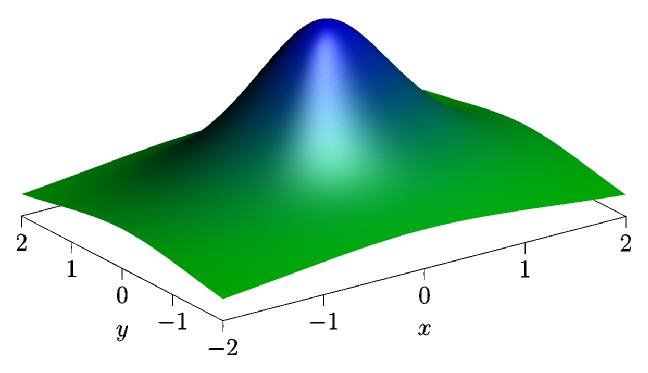
\includegraphics[width=12cm]{figure37.eps}
\caption{The graph of $f(x,y) = \frac{5}{x^2 + y^2 + 1}$}
\label{figure-3d-graph1}
\end{figure}

We used graphs extensively in single-variable calculus to
understand derivatives and integrals: derivative were slopes
of tangent lines and integrals were area under curves. We want
to generalize this to the new higher-dimensional graphs.  For
functions $f:\RR^2 \rightarrow \RR$, it's not too difficult to
extend the notions. Instead of tangent line, we now have
\emph{tangent planes}. Instead of area under the curve, we
have volume under the surface.  For $f: \RR^n \rightarrow
\RR$, we have tangent n-spaces and (n+1)-hyper-volume under
the n-dimensions graph surface. 

\subsection{Contour Plots}
\label{contour-plots}

As an alternative to conventional graphs of function, a nice
way to visualize height functions is as topological maps. We
refer to these visualizations as contour plots. 

\begin{defn}
Let $f: A \rightarrow \RR$ be a scalar function for a domain
$A \subset \RR^2$. A \emph{countour plot} for $f$ is a plot
of curves in $\RR^2$ where each curve is a locus of the form
$f(x,y) = c$ for some constant $c$.
\end{defn}

A contour plot has a series of implicit curves at constant
elevation; the constants $c$ are the elevation. It shows
curves where the function takes a specific value. By looking
at the relationships of the curves, we can intuit how the
function behaves.

\begin{example}
Consider $f(x,y) = \frac{5}{x^2+y^2+1}$. It's graph is Figure
\ref{figure-3d-graph1}. This function has
a simple hill at the origin and slopes down in all direction.
The contours are loci of the form $\frac{5}{x^2 + y^2 + 1} =
c$, which can be rearranged as $\frac{5}{c} - 1 = x^2 + y^2$.
These contours are all circles, and are shown in Figure
\ref{figure-contour-plot1}.
\end{example}

\begin{figure}[t]
\centering
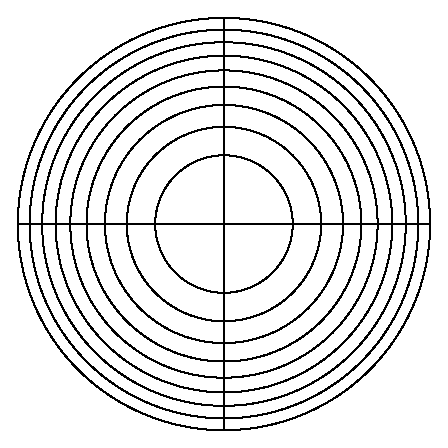
\includegraphics[width=7cm]{figure32.eps}
\caption{The circular contours of $f(x,y) = \frac{5}{x^2 + y^2
+ 1}$}
\label{figure-contour-plot1}
\end{figure}

\begin{example}
Contour diagrams can show many behaviours. Figure
\ref{figure-contour-plot2} shows a pass or saddle point. (The saddle
point will be formally defined in Definition
\ref{def-saddle-point}. 
\end{example}

\begin{figure}[ht]
\centering
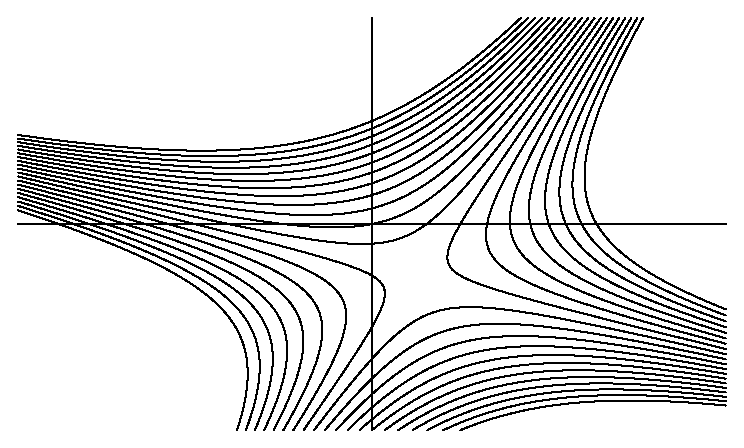
\includegraphics[width=12cm]{figure34.eps}
\caption{The contours of a saddle point}
\label{figure-contour-plot2}
\end{figure}

These contour plots lead us to a general definition.

\begin{defn}
Let $f: \RR^n \rightarrow \RR$ be a scalar function. A
\emph{level set} for $f$ is a subset of $\RR^n$ given by the
equation $f(x_1, x_2, \ldots, x_n) = c$ for some $c \in \RR$.
\end{defn}

Then a countour plot is just a drawing of a variety of level
sets of a function $\RR^2 \rightarrow \RR$. It is useful to
see where a function is constant. The resulting shapes tell
us a great deal about the behaviour of the function. Level
sets for $f: \RR^3 \rightarrow \RR$ are called level surfaces.

\section{Limits of Multivariable Functions}
\label{limits}

We want to re-establish the tools of calculus for
multi-variable functions. As with single-variable functions,
our starting point is limits. Let's start with the full,
formal, $\epsilon-\delta$ definition.

\begin{defn}
Let $f: \RR^n \rightarrow \RR$ be a function. Let $(a_1, a_2,
\ldots, a_n)$ be a point in $\RR^n$. Then the statement
\begin{equation*}
\lim_{(x_1, x_2, \ldots, x_n) \rightarrow (a_1, a_2, \ldots,
a_n)} f(x_1, x_2, \ldots, x_n) = L
\end{equation*}
means that $\forall \epsilon > 0$ $\exists \delta > 0$ such
that if $|(x_1, x_2, \ldots, x_n) - (a_1, a_2, \ldots, a_n)| <
\delta$ then $|f(x_1, x_2, \ldots, x_n) - L| < \epsilon$. 
\end{defn}

The definition is essentially the same as the single-variable
definition: as the input gets closer and closer to a specific
point, the output gets closer and closer to a fixed value $L$.
The only issue is that `closer and closer' now happens in
$\RR^n$ instead of $\RR$. 

In $\RR$, we only had two directions of approach: from the left
and from the right. If the behaviour from both sides was the
same, we said the limit existed. In $\RR^n$ for $n \geq 2$,
we have infinitely many ways to approach any given point. We
can approach along lines in infinitely many directions out from
the point. Even more, we can approach along other paths, such
as spiral paths or stranger jagged paths. This makes it much
more difficult to determine the behaviour and much
more difficult to prove existence of various limits. However,
we do have some good news. First, the definition of
continuity remains the same.

\begin{defn}
A function $f: \RR^n \rightarrow \RR$ is called continuous at
$(a_1, a_2, \ldots, a_n)$ if the limit approaching $(a_1,a_2,
\ldots, a_n)$ exists and is the same as $f(a_1,a_2, \ldots,
a_n)$.
\end{defn} 

So limits for continuous functions are still reasonable: we
just evaluate. But what functions are continuous?

\begin{prop}
A function $f: \RR^n \rightarrow \RR$ is continuous if and
only if it is continuous independently in each of its
variables.
\end{prop}

This is the first application of a very important technique:
treating the function as a function of only one of the
variables and ignoring the other, pretending that they are
constant. If we do that, we get $n$ different single variable
functions. The proposition says that the function is
continuous in the new definition if and only if all of the $n$
different single variable functions are continuous.

This proposition tells us how to recognize continuous
functions.  Anything involving polynomials, roots, rational
functions, trig, exponentials and logarithms is continuous on
its domain.

As we mentioned before, proving the existence of limits is
difficult. However, the algebraic techniques of first year
calculus can still work for calculations. Here are some
examples.

\begin{example}
\begin{align*}
\lim_{(x,y) \rightarrow (0,0)} \frac{x^2 - y^2}{x-y} & = 
\lim_{(x,y) \rightarrow (0,0)} \frac{(x-y)(x+y)}{(x-y)} \\
& = \lim_{(x,y) \rightarrow (0,0)} x+y = 0 + 0 = 0 \\
\lim_{(x,y) \rightarrow (4,1)} \frac{ xy - 4y^2}{\sqrt{x} -
2\sqrt{y}} & = 
\lim_{(x,y) \rightarrow (4,1)} \frac{y(\sqrt{x} -
2\sqrt{y})(\sqrt{x} + 2 \sqrt{y})}{\sqrt{x} - 2\sqrt{y}} \\
& = \lim_{(x,y) \rightarrow (4,1)} \sqrt{x} + 2 \sqrt{y} =
\sqrt{4} + 2 \sqrt{1} = 2 + 2 = 4 
\end{align*}
\end{example} 

\begin{figure}[t]
\centering
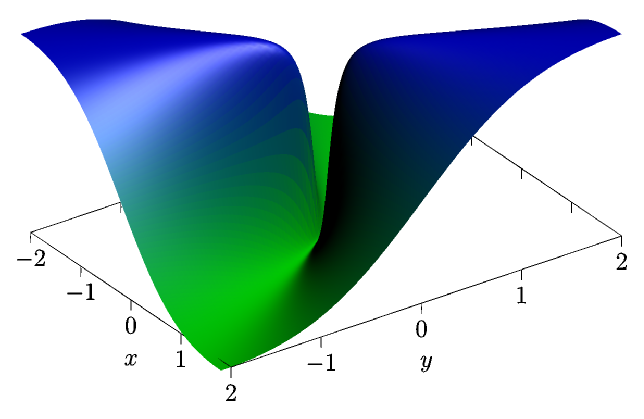
\includegraphics[width=12cm]{figure38.eps}
\caption{The graph of $f(x) = \frac{(x+y)^2}{x^2+y^2}$}
\label{figure-3d-graph2}
\end{figure}

\begin{example}
\begin{equation*}
\lim_{(x,y) \rightarrow (0,0)} \frac{(x+y)^2}{x^2 + y^2} 
\end{equation*}
Let's approach this along the line $y = mx$. That lets us
replace $y$ with $mx$ in the calculation and the limit becuase
$x \rightarrow 0$.
\begin{align*}
\lim_{x \rightarrow 0} \frac{(x+mx)^2}{x^2 + m^2x^2}
& = \lim_{x \rightarrow 0} 
\frac{x^2 + 2mx + m^2 x^2}{x^2 + m^2 x^2} \\
& = \lim_{x \rightarrow 0}
\frac{x^2(1+m)^2}{x^2(1+m^2)} = \frac{(1+m)^2}{1+m^2}
\end{align*}
This limit depend on the choice of $m$!
We can get infinitely many values (all between 0
and 1) out of this limit depending on which line we use to
approach $(0,0)$. With all these possible answers, the limit
cannot exist. It is interesting to try to visualize the graph:
as we get close to zero, there are pieces of the graph getting
close to any number between $0$ and $1$. Figure \ref{figure-3d-graph2}
shows some of this behaviour: approaching from the front of
figure leads to $0$, but approaching from the sides leads to
larger numbers. (The graph is slightly flawed, due to
the graphing algorithm. The two cliffs should meet, even
though the graph shows a gap between them. Where the two
cliffs meet is the line with all the problematic limits.)
\end{example}

\begin{example}
In this example, we approach along parabolic paths of the form
$ x = m y^2$ and, like the previous example, get a limit that
depends on the path of approach. 
\begin{equation*}
\lim_{(x,y) \rightarrow (0,0)} \frac{3xy^2}{x^2 + y^2} = 
\lim_{(x,y) \rightarrow (0,0)} \frac{3xy^2}{x^2 + y^2} 
= \lim_{y \rightarrow 0} \frac{3my^4}{m^2 y^4 + y^4}
= \frac{3m}{m+1} 
\end{equation*}
\end{example}

\begin{example}
\begin{align*}
\lim_{(x,y) \rightarrow (1,2)} \frac{\sqrt{y} -
\sqrt{x+1}}{y-x-1} & = 
\lim_{(x,y) \rightarrow (1,2)} \frac{y-x-1}{(y-x-1)(\sqrt{y} +
\sqrt{x+1})} \\
& = \frac{1}{\sqrt{2} + \sqrt{2}} = \frac{1}{2\sqrt{2}} 
\end{align*}
\end{example}

\begin{example}
Sometime we can make reasonable conclusion independent of
path. 
\begin{equation*}
\lim_{(x,y) \rightarrow (0,0)} \frac{\sin(x+y)}{x+y} 
\end{equation*}
We can assume any path $y = f(x)$ of approach and still set $u
= x+y$, which turns this into a limit of $\sin(u)/u$, which
tends to 1.
\end{example}

\section{Partial Derivatives}
\label{partial-derivatives}

The first of several generalizations of derivatives is the
partial derivative. 

\begin{defn}
Let $f: \RR^n \rightarrow \RR$ be a scalar function. If $x$ is
one of the variable, then the derivative of $f$ which pretend
that all other variables are constant is called the
\emph{partial derivative} of $f$ in the variable $x$. 
\end{defn}

The notation for partial derivatives resembles Leibniz
notation for ordinary derivatives: $\frac{df}{dx}$. Leibniz
style notation is useful since the variable of differentiation
is explicit.  The partial derivatives of $f$ in terms of $x$,
$y$, $z$, or $x_i$ are written with a stylized version of $d$
in Leibniz notation.
\begin{equation*}
\frac{\del f}{\del x} \hspace{1cm} 
\frac{\del f}{\del y} \hspace{1cm} 
\frac{\del f}{\del z} \hspace{1cm} 
\frac{\del f}{\del x_1} 
\end{equation*}

For interpretation, this gives us the rate of change of $f$
with respect to one of its variables. We don't have a
holisitic notion of rate of change, but we can see how it
changes in each variable. 

If we wanted to be formal, pretending that all the other
variales are constant is the same as taking limits in one
variable.  For $f: \RR^2 \rightarrow \RR$, these limits
defined the two partial derivatives.
\begin{align*}
\frac{\del f}{\del x} (a,b) & = \lim_{(x,y) \rightarrow (a,b)}
\frac{ f(a+h, b) - f(a,b)}{h} \\
\frac{\del f}{\del y} (a,b) & = \lim_{(x,y) \rightarrow (a,b)}
\frac{ f(a, b+h) - f(a,b)}{h} \\
\end{align*}
Notice that the value of $\frac{\del f}{\del x}$ still depends
on $y$. Different $y$ values identify different point in the
domain, where the rate of change with respect to $x$ may
differ. 

\begin{defn}
A function $f: \RR^n \rightarrow \RR$ is \emph{differentiable} at
$(a_1, a_2, \ldots, a_n)$ if \emph{all} of its partial
derivatives $\frac{\del f}{\del x_i}$ exists at that point.
\end{defn}

As we did for single-variable calculus, we use
$\frac{\del}{\del x}$ and similar expressions as operators --
the things that take derivatives.

There are various notational conventions for partial
derivatives. In addition to $\frac{\del f}{\del x}$, we can
also write this as $f_x$, $\del_x f$ and $D_x f$. The first
of these is a nice short-hand which we will use frequently.

\begin{example}
\begin{align*}
f(x,y) & = x^2 + y^2 \sin x \hspace{2cm}
\frac{\del f}{\del x} = 2x + y^2 \cos x \hspace{2cm}
\frac{\del f}{\del y} = 2y \sin x \\[1em]
f(x,y) & = \frac{1}{xy + e^{xy}} \hspace{2cm}
\frac{\del f}{\del x} = \frac{-1}{x^2y} + xe^{xy} \hspace{2cm} 
\frac{\del f}{\del y} = \frac{-1}{xy^2} + ye^{xy} 
\\[1em]
f(x,y) & = \frac{x^2y^2+xy}{x^2 + y^2 + 1} \\
\frac{\del f}{\del x} & = \frac{(2xy^2+y)(x^2 + y^2 -1 ) -
(x^2 + y^2 + xy)(2x)}{(x^2 + y^2 + 1)^2} \\
\frac{\del f}{\del y} & = \frac{(2x^2y + x)(x^2+ y^2 -1 ) -
(x^2 y^2 + 2y)(2y)}{(x^2 + y^2 + 1)^2}
\end{align*}
\end{example}

\begin{example}
We can also take higher partial derivatives.
\begin{displaymath}
\begin{array}{*4{>{\displaystyle}l}}
f(x,y) & = 3x^3 y^2 - xy^4 + x^2 y^3 - 3 & & \\[1em]
\frac{\del f}{\del x } & = 9x^2y^2 - y^4 + 2xy^3 & 
\hspace{2cm} \frac{\del f}{\del y } & = 6x^3y - 4xy^3 + 2x^2y
\\[1em]
\frac{\del^2 f}{\del x^2 } & = 18xy^2 + 2y^3 &
\hspace{2cm} \frac{\del^2 f}{\del y^2 } & = 6x^3 - 12xy^2 +
2x^2 \\[1em]
\frac{\del^3 f}{\del x^3 } & = 18y^2 &
\hspace{2cm} \frac{\del^3 f}{\del y^3 } & = -24xy \\ [1em]
\frac{\del^4 f}{\del x^4 } & = 0 &
\hspace{2cm} \frac{\del^4 f}{\del y^4 } & = -24x \\[1em]
\frac{\del^5 f}{\del x^5 } & = 0 &
\hspace{2cm} \frac{\del^5 f}{\del y^5 } & = 0 
\end{array}
\end{displaymath}
\end{example}

\begin{example}
In addition, we can mix the partial derivatives, first taking
the partial in $x$ and the in $y$ or vice-versa. 
\begin{align*}
\frac{\del}{\del y} \frac{\del f}{\del x} = \frac{\del^2
f}{\del y \del x} = 18x^2y - 4y^3 + 4xy \\
\frac{\del}{\del x} \frac{\del f}{\del y} = \frac{\del^2
f}{\del x \del y} = 18x^2y - 4y^3 + 4xy 
\end{align*}
Curiously, we get the same answer from either order of the
mixed partial derivatives. This equality is true in general
and is called Clairaut's Theorem. In the statement of the
proposition, notice the requirement that the domain is an open
set. This is an example of the topological conditions invovled
in multivariable calculus. 
\end{example}

\begin{prop}
Let $f(x,y)$ be a function $\RR^2 \rightarrow \RR$. If all the
partial derivatives $f_{xx}$, $f_{yy}$, $f_{xy}$ and $f_{yx}$
exists and are continuous on an open set $D$, then $f_{xy} =
f_{yx}$ on that set.
\end{prop}

\section{Partial Differential Equations}
\label{pdes}

\begin{figure}[ht]
\centering
\includegraphics[width=12cm]{figure39.eps}
\caption{Concavity and Heat Diffusion}
\label{figure-concavity-heat}
\end{figure}

Now that we have defined partial derivatives, we can introduce
what is possibly the most important setting for their use:
partial differential equations. We can start with two classic
examples. The first is diffusion of heat.

Let's say we have a 1-dimensional rod where length is measured
with the variable $x$. Heat can vary along the rod, so we
measure it by a function $u(x)$. However, this distribution of
heat can also change over time. Therefore, we should measure
the heat distribution both in terms of position $x$ along the
rod and time $t$, $u(x,t)$.

We need to consider several aspects of the situation to give a
full account of how heat will diffuse. First, let's look at
the mechanics of heat. We make the assumption that heat wants
to equalize; with the absence of external addition of heat, it
will diffuse until it equals out everywhere. If addition, we
assume that the greater the variance in heat between two
adjacent points on the rod, the faster the heat will diffuse.
How do we translate this assumptions into mathematics? We
need to get a measure of this variance in heat. The measure
is local, since heat only diffuses to points adjacent. So how
do we meausre how much local variance there is in heat? 

Consider the heat picture at some fixed time $t_0$:
$u(x,t_0)$. It is not the value of the heat that determines
diffusion, since nearby values can be higher or lower. It is
also not the slope of this graph in $x$ that determines the
diffusion, since a straight line slope represents and even
flow of heat from one end to the other. We can think of heat
wanting to return to this even flow, this straight line: so it
is the curvature of the graph that disrupts the straight line.
Curvature or concavity is measured by the second derivative.
Therefore $u_{xx}(x,t_0)$ measures the tendency for the heat to
diffuse. Figure \ref{figure-concavity-heat} illustrates how concavity
causes heat diffusion. 

Diffusion creates change: heat will leave or enter the point.
Change is measured by the time derivatives $u_t(x,t)$. So
convacity, the second space deriavitve, must be related to the
first time derivative. What is the relationship between these?
Let's assume the simpliest case for now and make the
relationship linear. That means there is a constant $\alpha$
such that 
\begin{equation*} 
\frac{\del u}{\del t} = \alpha \frac{\del^2 u}{\del x^2}.  
\end{equation*} 
This equation is called the Heat Equation. Though relatively
simple, it is one of the most important partial differential
equations.

The equation, however, isn't enough to solve the problem. We
also need boundary conditions and initial conditions. The
boundary conditions tell us what happens at the end of the
rod: $u(0,t)$ and $u(l,t)$. In principle, these could be
anything functions of $t$. For now, let's assume they are
constant $u(0,t) = a$ and $u(l,t) = b$. 

We also need intial conditions. These tells us the starting
heat distribution at at particular time, say $t=0$, That is
$u(x,0) = f(x)$, a single variable function that tells us the
original situation. 

All together, this information determines the physical system.
We can then try to find a function $u(x,t)$ which matches the
equation, the boundary conditions and the initial conditions.
Such a task is often very difficult to do. However, if both
boundary conditions are constant $0$ and the initial condition
is $f(x) = \sin \left( \frac{\pi x}{l} \right)$ then the
function 
\begin{equation*}
u(x,t) = e^{-\frac{\alpha \pi^2 t}{l^2}} \sin \left( \frac{\pi
x}{l} \right)
\end{equation*}
solves the partial differential equation. This is an ideal
case: in general the solutions become much more complicated.
This initial heat distribution is half a period of a sine wave,
and the time dependence is a exponential decay of the
amplitude of that sine wave back towards a stable 0-level heat
distribution.

This example is archtypical of many partial differential
equations. We will almost always have a function which
depends on time as well as some other quantities. In physics,
these other quantities are usually position. Then the
equation is usually organized by taking a time derivative on
one side and a position derivative on the other. Then we posit
a relationship between the two two derivatives. In addition,
boundary conditions tell us what happens at the edges of our
environment and initial conditions give us a snapshot of the
situation at a fixed moment in time. Then we try to find a
multi-variable function that fits all the information.

Another very familiar situation is a wave moving through an
elastic medium. We'll assume a 1-dimensional elastic medium
(think a wire or string), then $u(x,t)$ measures the
displacement of the medium at position $x$ and time $t$. The
physical motivation is similar to the heat equation: the
concavity measure the offset of the stiuation from a stable
straight line. However, this concavity, instead of causing
heat diffusion, causes acceleration on the adjacent points of
the elastic medium. The elastic medium doesn't diffuse back
to equilibrium, it accelerates, like a spring, back to
equilibrium. Acceleration is a second time derivative, so
the Wave Equation is
\begin{equation*}
\frac{\del^2 u}{\del t^2} = \alpha \frac{\del^2 u}{\del x^2}.
\end{equation*}
Again, there are boundary conditions and initial condition
and, in general, the problem is very difficult to solve.
However, if we take the same situation as before, with
constant zero boundary conditions at $x=0$ and $x=l$ and
initial wave profile $f(x) = \sin \left( \frac{ \pi x}{l}
\right)$, then the solution is
\begin{equation*}
u(x,t) = \sin \left( \frac{\sqrt{\alpha} \pi t}{l} \right)
\sin \left( \frac{\pi x}{l} \right).
\end{equation*}
So, instead of decay to equilibrium, we get an oscillating
amplitude, resulting is a very simple standing wave on the
wire or string. This is a very simple version: there are no
higher harmonics and there is no friction which causes decay
over time.

Many other famous equations are relationships between times
derivatives and position derivatives. In all of the following
examples, the left side is a time derivative and the right is
a space derivative.

In classical Newtonian mechanics, for conservative forces like
gravity and electromagnetism, the force is often determined by
a potential energy field $V$.
\begin{equation*}
F = - \frac{d V(x)}{dx}
\end{equation*}
But $F = ma$ is Newton's first law, and acceleration is a time
derivative of position. 
\begin{equation*}
\frac{d^2 x}{dt^2} = \frac{-1}{m} \frac{dV}{dx}
\end{equation*}
The Schrodinger equation is the centre of quantum mechanics:
it measures a wave function $\Psi(x,y,z,t)$ in three
dimensions and time. The symbol $\nabla$ is a 3-dimemsional
differential operator which will be defined later; for now,
just know that it is a combination of position derivatives.
$\hbar$ is a constant, $\imath$ is a number with $\imath^2 =
-1$, $m$ is mass and $V(x,y,z)$ is a potential energy
function. 
\begin{equation*}
\imath \hbar \frac{\del \Psi}{\del t} = - \frac{ \hbar^2}{2m}
\nabla^2 \Psi + V \Psi
\end{equation*}
Another famous example is the Navier-Stokes equation, which is
the fundamental equation of fluid dynamics. There are a
number of versions of it, but I'll only write one. The
function $v(x,y,z,t)$ is the flow velocity of a
three-dimensional fluid. Again, $\nabla$ is a 3-dimensional
position differential operator. $\rho$ is the fluid density,
$p$ is the pressure, $T$ is something called a stress tensor
and $f$ is an external force of the fluid. The equation is
\begin{equation*}
\rho \frac{\del v}{\del t} = \rho v \cdot \nabla v - \nabla p
+ \nabla \cdot T + f
\end{equation*}
Solving the Navier-Stokes equation for various initial and
boundary conditions is the subject of a whole branch of
mathematical physics called fluid dynamics. 

\section{Gradients}
\label{gradients}

After partial derivatives, we want to proceed to define
several other generalizations of the derivative. The first is
the gradient. 

\begin{defn}
The gradient of a function $f: \RR^n \rightarrow \RR$ is
written $\nabla f$ and defined as
\begin{equation*}
\nabla f = \left( \frac{\del f}{\del x_1}, \frac{\del f}{\del
x_2}, \ldots, \frac{\del f}{\del x_n} \right)
\end{equation*}
\end{defn}

The gradient is a new function $\RR^n \rightarrow \RR^n$. It
ouputs the \emph{vector} of partial derivatives of $f$ at any
point in its domin. Note that the gradient is a local
direction vector \emph{in the domain}. 

The best interpretation of the gradient comes from contour
plots. Like the gradient, countour plots live in $\RR^n$, the
domain, and show the level (hyper)surfaces of the function.
If, as in $\RR^2$, we think of the function as a height
function and the countour plot as a topographical map, the
gradient shows direction of greatest increase. 

If we draw topographical lines on a countour plot, the
gradient will always be locally perpendicular to those lines
and will point in the direction of greatest increase.
Rephrased, this is a useful result: $\nabla f$ is always the
normal to the level sets of $f$. If those level sets are
hypersurfaces, their tangent planes can be determined by the
normal $\nabla f$. 

\begin{example}
A central example of gradients is found by considering the
gravitational potential energy function caused by a mass $m$
at the the origin. Another object of mass $m$ and
position $(x,y,z)$ has potential gravitational energy of
\begin{equation*}
P = \frac{-GmM}{\sqrt{x^2 + y^2 +z^2}}.
\end{equation*}
By convention, this potential energy is negative. It
approaches $0$ in the limit at the origin, and approaches $-
\infty$ as we get very far from the origin. The gradient of
this is 
\begin{equation*}
\nabla P = \frac{GmM}{\sqrt{(x^2 + y^2 +z^2)^3}} (x, y, z) =
\frac{GmM}{x^2 + y^2 + z^2} \frac{1}{\sqrt{x^2 + y^2 + z^2}}
(x,y,z).
\end{equation*}
This is precisely the force of gravity. The gradient point in
the direction of maximum increase in potential energy with
magnitude $\frac{GmM}{r^2}$ where $r$ is the distance between
the two objects. This is a common situation we will discuss
in Calculus IV: many forces are the result of gradients of
potential energy functions. 
\end{example}

\begin{example}
In another example, consider a function $p(x,y,z)$ which
measures the pressure in a rotating cylindrial drum. (Think
of a centrifuge). With bounds $z \in [0,5]$ and $x,y \in [0,
\sqrt{3}]$, the function is 
\begin{equation*}
p(x,y,z) = \frac{1}{z+1} (x^2 + y^2)
\end{equation*}
The gradient is
\begin{equation*}
\nabla p(x,y,z) = \left( \frac{2x}{z+1}, \frac{2y}{z+1},
\frac{-(x^2 + y^2)}{(z+1)^2} \right)
\end{equation*}
This points in the direction of greatest increase in pressure.
It is perpendicular to the surfaces of constant pressure. If
there is a difference in media in the drum, the lighter medium
will be force towards the edges of the drum in the direction
of this gradient. 
\end{example}

In addition to the gradient, we can think of $\nabla$ itself
as the following differential operator.
\begin{equation*}
\nabla = \left( 
\frac{\del}{\del x_1}, 
\frac{\del}{\del x_2}, 
\frac{\del}{\del x_3}, \ldots, 
\frac{\del}{\del x_n} \right) 
\end{equation*}
This is a vector-valued differential operator: it outputs the
vector of partial derivatives $\nabla f$. Now that
we have this operator, there are other operations we can use
it for. Most of those operations come in Calculus IV, but we
can define one such operation here. 

\begin{defn}
If $f: \RR^n \rightarrow R$ is a scalar function, the
\emph{Laplacian} of $f$ is given by applying $\nabla$ twice.
Since $\nabla$ outputs a vector, the second application uses
the dot product to output a scalar. 
\begin{align*}
\nabla^2 f & = \nabla \cdot \nabla f = \left( 
\frac{\del}{\del x_1}, 
\frac{\del}{\del x_2}, 
\frac{\del}{\del x_3}, \ldots, 
\frac{\del}{\del x_n} \right) 
\cdot \left( \frac{\del f}{\del x_1}, 
\frac{\del f}{\del x_2}, 
\frac{\del f}{\del x_3}, \ldots, 
\frac{\del f}{\del x_n} \right) \\
& = 
\frac{\del^2 f}{\del^2 x_1} + 
\frac{\del^2 f}{\del^2 x_2} +
\frac{\del^2 f}{\del^2 x_3} + \ldots 
\frac{\del^2 f}{\del^2 x_n} 
\end{align*}
\end{defn}

The Laplacian, as a second derivative, measure some kind of
multi-dimensional concavity. We considered the heat equation
in one dimension; in that equation, concavity measured local
displacement from equilibrium. The Laplacian does the same in
multiple dimensions. The general Heat Equation is
\begin{equation*}
\frac{\del u}{\del t} = \alpha \nabla^2 u.
\end{equation*}
Similarly, the general Wave Equation is
\begin{equation*}
\frac{\del^2 u}{\del t^2} = \alpha \nabla^2 u.
\end{equation*}

\section{Directional Derivatives}
\label{directional-derivatives}

Partial derivatives took one variable and pretended that all
other variables were constant. In that way, we got the rate of
change in that variable. We could consider $\frac{\del f}{\del
x}$ the derivative of $f$ \emph{when we move} in the $x$ axis 
direction. But why do we only need to move in the axis
direction? Why can't we move in all directions and consider
the rate of change?

\begin{defn}
Let $f: \RR^n \rightarrow \RR$ be a differentiable function
and $u$ a \emph{unit} vector in $\RR^n$. The directional
derivative of $f$ in the direction $u$ is written $D_u
f$ and given by a limit definition. Let $v$ be a point in the
domain of $f$. 
\begin{equation*}
D_u f(v) = \lim_{h \rightarrow 0} \frac{ f(v + hu) - f(v)}{h}
\end{equation*}
\end{defn}

The directional derivative, like the partial derivative,
uses a single variable limit: we use the line in
the direction $u$ (as a local direction vector form the point
$v$) to give a one-dimensional domain -- a copy of $\RR^1$.
Then we just differentiate along the line. If $u = e_1$, we
get $D_{e_1} f = f_{x_1}$. If $u = e_2$ we get $D_{e_2} f =
f_{x_2}$ and so on. 

Instead of calculating this limit every time, we have a nice
tool for calculating directional derivatives.
\begin{prop}
Let $f: \RR^n \rightarrow \RR$ be a differentiable function
and $u$ a \emph{unit} vector in $\RR^n$. The directional
derivatives $D_u f$ is the dot product of $u$ with $\nabla f$. 
\begin{equation*}
D_u f = u \cdot \nabla f
\end{equation*}
\end{prop}

\begin{figure}[t]
\centering
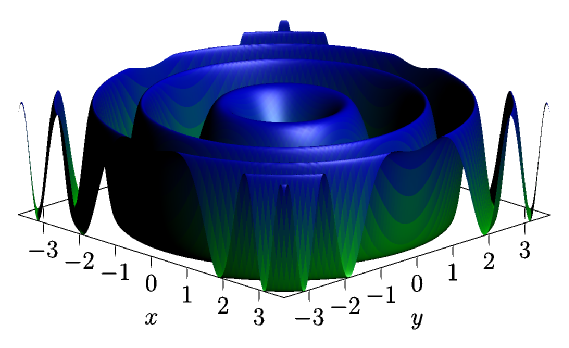
\includegraphics[width=12cm]{figure40.eps}
\caption{The function $f(x,y) = \sin (x^2 + y^2)$.}
\label{figure-3d-graph3}
\end{figure}

If $(a,b)$ or $(a,b,c)$ are unit vectors in $\RR^2$ and
$\RR^3$, respectively, we can write the specific form of the
proposition for low dimensions. 
\begin{align*}
D_{(a,b)} f(x,y) & = 
\frac{\del f}{\del x} a + 
\frac{\del f}{\del y} b \\
D_{(a,b,c)} f(x,y,z) & = 
\frac{\del f}{\del x} a + 
\frac{\del f}{\del y} b + 
\frac{\del f}{\del z} c 
\end{align*}

As we noted above, the directional derivatives in the axis
directions give the partial derivatives, so this is an
extension of the idea of partial derivatives. 
\begin{align*}
D_{(1,0)} f(x,y) & = \frac{\del f}{\del x} \\
D_{(0,1)} f(x,y) & = \frac{\del f}{\del y} \\
D_{(1,0,0)} f(x,y,z) & = \frac{\del f}{\del x} \\
D_{(0,1,0)} f(x,y,z) & = \frac{\del f}{\del y} \\
D_{(0,0,1)} f(x,y,z) & = \frac{\del f}{\del z} 
\end{align*}

\begin{figure}[t]
\centering
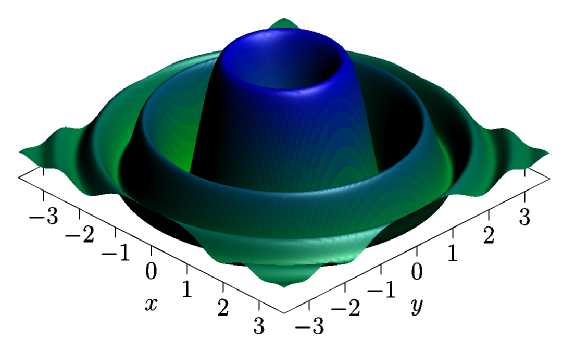
\includegraphics[width=12cm]{figure41.eps}
\caption{The function $f(x,y) = e^{-(x^2+y^2)}\sin (x^2 + y^2)$.}
\label{figure-3d-graph4}
\end{figure}

\begin{example}
Consider this function: $f(x,y) = \sin (x^2 + y^2)$, show in
Figure \ref{figure-3d-graph3}. These are circular sine waves, like
riples on a pond which never decrease in amplitude. We have
\begin{align*}
D_{(1,0)} f(x,y) & = 2x \cos (x^2 + y^2) \\
D_{(0,1)} f(x,y) & = 2y \cos (x^2 + y^2) \\
D_{ \left( \frac{1}{\sqrt{5}} , \frac{2}{\sqrt{5}} \right) } 
f(x,y) & = \frac{2}{\sqrt{5}} x \cos (x^2 + y^2) +
\frac{2}{\sqrt{5}}y \cos (x^2 + y^2)\\
D_{ \left( \frac{1}{\sqrt{5}} , \frac{2}{\sqrt{5}} \right) }
f(\sqrt{\pi},\sqrt{\pi}) & =
\frac{2}{\sqrt{5}} \sqrt{\pi} \cos (\pi + \pi) +
\frac{2}{\sqrt{5}} \sqrt{\pi} \cos (\pi + \pi) = 4 \sqrt{
\frac{\pi}{5}} \\
\end{align*}
If we wanted damped ripples instead, as in Figure
\ref{figure-3d-graph4}, we would take $f(x,y) = e^{-(x^2 + y^2)}
\sin(x^2 + y^2)$. 
\begin{align*}
D_{(a,b)} f(x,y) & = \left[ -2xe^{-(x^2+y^2)} \sin (x^2 + y^2) +
2xe^{-(x^2+y^2)} \cos (x^2 + y^2) \right] a \\
& \hspace{1cm} + \left[ -2ye^{-(x^2+y^2)} \sin (x^2 + y^2) +
2ye^{-(x^2+y^2)} \cos (x^2 + y^2) \right] b \\
D_{(a,b)} f(\sqrt{\pi},\sqrt{\pi}) & = 
\left[ -2\sqrt{\pi}e^{-(\pi+\pi)} \sin (\pi + \pi) +
2\sqrt{\pi}e^{-(\pi+\pi)} \cos (\pi + \pi) \right] a \\
& \hspace{1cm} + 
\left[ -2\sqrt{\pi}e^{-(\pi + \pi )} \sin (\pi + \pi ) +
2\sqrt{\pi}e^{-(\pi + \pi )} \cos (\pi + \pi) \right] b \\
& = \frac{2\sqrt{\pi}}{e^{2\pi}} \left[ \cos (2\pi) a + \cos
(2\pi) b \right] = \frac{2 \sqrt{\pi} (a+b)}{e^{2\pi}}
\end{align*}
\end{example}

Finally, look at what happens when we apply the length of a
dot product to the directional derivative. 
\begin{equation*}
|D_u f| = |\nabla f \cdot u| = |\nabla f||u| \cos \theta
\end{equation*}
The cosine term is maximized when the angle $\theta =0$,
that is, when $u$ is the unit vector in the same direction as
$\nabla f$. That is, the greatest directional derivative,
representing the direction of fastest change, is found in the
direction of the gradient. This established the fact, which we
claimed earlier, that the gradient points in the direction of
greatest change. 

\section{The Chain Rule}
\label{chain-rule}

We defined partial derivatives to measure rates of change in a
particular variable. We extended this to change in any unit
direction with directional derivatives. We can extend this
even further, but considering the change in a function as we
move along a \emph{parametric curve} in the domain. 

Let $f(x,y,z): \RR^3 \rightarrow\RR$, be a potential energy
function. Let $\gamma(t) = (x(t), y(t), z(t))$ be a curve
moving through $\RR^3$.  If this is a potential energy
function, we want to know how quickly we gain and/or lose
energy moving along the path $\gamma$. The energy along
$\gamma$ is $f(\gamma(t)) = f(x(t), y(t), z(t))$. The rate of
change is $\frac{df}{dt}$.  But now $f$ is a composition,
$f(\gamma(t))$, so this must be a chain rule calculation. What
is the chain rule when we have three (or more) components?.

\begin{prop}
(The Chain Rule) Let $f: \RR^n \rightarrow \RR$ be a scalar
function and $\gamma(t)$ a parametric curve in $\RR^n$ inside
the domain of $f$. The derivative of $f$ along $\gamma$ is 
\begin{equation*}
\frac{d}{dt} f(\gamma(t)) = 
\frac{\del f}{\del x_1} \frac{dx_1}{dt} + 
\frac{\del f}{\del x_2} \frac{dx_2}{dt} + \ldots + 
\frac{\del f}{\del x_n} \frac{dx_n}{dt} 
\end{equation*}
The total rate of change is the sum of the rates of changes in
each of the variables. 
\end{prop}

For reference, here is the chain rule in $\RR^3$.
\begin{equation*}
\frac{d}{dt} f((x(t), y(t), z(t)) = 
\frac{\del f}{\del x} \frac{dx}{dt} + 
\frac{\del f}{\del y} \frac{dy}{dt} + 
\frac{\del f}{\del z} \frac{dz}{dt} 
\end{equation*}

\begin{example}
Consider the potential gravitational energy function 
\begin{equation*}
P = - \frac{GmM}{r} = \frac{-GmM}{\sqrt{x^2 + y^2 + z^2}}
\end{equation*}
If we move along a curve $\gamma$, it is nice to know how the
potential energy changes. A helical path out of the gravity
well might be $\gamma(t) = (\sin t, \cos t, t)$. We
differentiate along this path using the chain rule. 
\begin{align*}
\frac{dP}{dt} & = 
\frac{\del P}{\del x} \frac{dx}{dt} + 
\frac{\del P}{\del y} \frac{dy}{dt} + 
\frac{\del P}{\del z} \frac{dz}{dt} \\
& = 
\frac{GmMx}{(x^2 + y^2 + z^2)^{\frac{3}{2}}} \frac{dx}{dt} + 
\frac{GmMy}{(x^2 + y^2 + z^2)^{\frac{3}{2}}} \frac{dy}{dt} + 
\frac{GmMz}{(x^2 + y^2 + z^2)^{\frac{3}{2}}} \frac{dz}{dt} \\
& = 
\frac{GmM\sin t}{(1 + t^2)^{\frac{3}{2}}} \cos t + 
\frac{GmM\cos t}{(1 + t^2)^{\frac{3}{2}}} (-\sin t) + 
\frac{GmMt}{(1 + t^2)^{\frac{3}{2}}} 1 \\
& = \frac{GmMt}{\sqrt{(1+t^2)^3}} 
\end{align*}
Notice that if we let $|\gamma(t)| = \sqrt{1 + t^2}$ at the
start, we could have written $P(t) = \frac{-GmM}{|\gamma(t)|} =
\frac{-GmM}{\sqrt{1+t^2}}$ and the $P^\prime(t) =
\frac{GmMt}{\sqrt{(1+t^2)^3}}$ could have been calculated
directly. That would have been easier, but its nice to get
confirmation that working with the chain rule leads to the
right result. 
\end{example}

\section{Tangent Planes}
\label{tangent-planes}

In single variable calculus, derivatives allowed us to find
the slopes and equations of tangent lines to the graph of a
function. We want to extend this idea. For functions of two
variables, we have graphs which are surfaces in $\RR^3$
instead of curves in $\RR^2$. These surfaces have tangent
planes instead of tangent lines.

If we have such a function $f(x,y)$ let's look at a particular
point $(a,b,f(a,b))$ on the graph of the function. We can
calculate the partial derivatives $f_x(a,b)$ and $f_y(a,b)$.
At the point $(a,b,f(a,b))$, these two partial derivatives
give us the rate of change in $x$ and in $y$. That's the
slope of a tangent line in the $x$ direction and a tangent
line in the $y$ direction. We'd rather have direction vectors
than slopes, but we can construct these. For the $x$
direciton, the $y$ coordinate is $0$ since there is no change
in $y$. That gives the vector $(1, 0, f_x(a,b))$. Likewise
in the $y$ direction, we have the vector $(0,1,f_y(a,b))$.
These are two tangent local direction vectors.

If we have two vectors on a plane, the normal of the plane is
given by the cross product. So we calculate $(1,0, f_x(a,b))
\times (0,1, f_y(a,b)) = (-f_x(a,b), -f_y(a,b),1)$. Therefore,
we have the following result.

\begin{prop}
Let $f(x,y)$ be a function $\RR^2 \rightarrow \RR$. The
equation of the tangent plane to $f$ at $(a,b,f(a,b))$ is 
\begin{equation*}
z - f(a,b) = f_x(a,b) (x-a) + f_y(a,b) (y-b)
\end{equation*}
\end{prop}

\begin{proof}
We just calculated the normal at any point $(a,b,f(a,b))$ on
the graph of the function. That vector was $(-f_x(a,b),
-f_y(a,b),1)$. From Section \ref{standard-forms} the equation
of the plane is given by the dot product of the variables with
the normal. Here is this dot product, with an unknown value
$c$. 
\begin{equation*}
- f_x(a,b) x - f_y(a,b) y + z = c
\end{equation*}
We have a point on the plane: $(a,b,f(a,b))$. By substitution,
we can solve for $c$.
\begin{equation*}
c = f(a,b) - f_x(a,b) a - f_y(a,b) b
\end{equation*} 
Putting this $c$ in gives the equation of the plane.
\begin{equation*}
- f_x(a,b) x - f_y(a,b) y + z = f(a,b) - f_x(a,b)a - f_y(a,b)b 
\end{equation*}
From here, is it just a re-arrangement to get the form in the
proposition. 
\end{proof}

\begin{example}
\label{example-tangent-plane}
Consider $f(x,y) = \frac{1}{1 + x^2 + y^2}$. 
\begin{equation*}
\frac{\del f}{\del x} = \frac{-2x}{(1+x^2+y^2)^2} \hspace{2cm}
\frac{\del f}{\del y} = \frac{-2y}{(1+x^2+y^2)^2} 
\end{equation*}
At the point $(x,y) = (1,1)$, we have $f_x(1,1) =
\frac{-2}{9}$ and $f_y(1,1) = \frac{-2}{9}$. The normal is
$\left( \frac{-2}{9}, \frac{-2}{9}, 1 \right)$ and the point
is $\left(1,1, \frac{1}{3} \right)$. The tangent plane is 
\begin{equation*}
\frac{2}{9} x + \frac{2}{9} y + z = \frac{7}{9}.
\end{equation*}
At the point $(x,y) = (0,0)$, we have $f_x(0,0) =
0$ and $f_y(0,0) = 0$. The normal is
$(0,0,1)$ and the point is $(0,0,1)$. The tangent plane is
\begin{equation*}
z=1.
\end{equation*}
At the point $(x,y) = (-2,2)$, we have $f_x(-2,2) =
\frac{4}{81}$ and $f_y(-2,2) = \frac{-4}{81}$. The normal is
$\left( \frac{-4}{81}, \frac{4}{81}, 1 \right)$ and the point
is $\left(-2,2, \frac{1}{9} \right)$. The tangent plane is 
\begin{equation*}
\frac{-4}{81} x + \frac{4}{81} y + z = \frac{1}{9}.
\end{equation*}
\end{example}

The definition of tangent planes for $f: \RR^2 \rightarrow
\RR$ extends to as many dimensions as we want. A function $f:
\RR^3 \rightarrow \RR$ has a graph in $\RR^4$. Its tangent
spaces are 3-spaces in $\RR^4$. We can understand those
3-spaces in a very similar method. We calcluate the three
local tangent directions. 
\begin{equation*}
v_1 = \left( 1, 0, 0, \frac{\del f}{\del x} \right)
\hspace{2cm}
v_2 = \left( 0, 1, 0, \frac{\del f}{\del y} \right)
\hspace{2cm}
v_3 = \left( 0, 0, 1, \frac{\del f}{\del z} \right) 
\end{equation*}
There isn't a cross-product in $\RR^4$, but we can genearlize
the pattern in this case to get the normal to the tangent
3-space. 
\begin{equation*}
\left( - \frac{\del f}{\del x}, - \frac{\del f}{\del y}, -
\frac{\del f}{\del z}, 1 \right)
\end{equation*}
The equation of the tangent 3-space at $(a,b,c,f(a,b,c))$ is 
\begin{equation*}
w - f(a,b,c) = \frac{\del f}{\del x}(a,b,c) (x-a) + \frac{\del
f}{\del y} (a,b,c) (y-b) + \frac{\del f}{\del z} (a,b,c) (z-c)
\end{equation*}
And we could extend this to $f: \RR^n \rightarrow \RR$, which
has a tangent hyperplane in $\RR^{n+1}$. 
\begin{equation*}
v_1 = \left( 1, 0, \ldots, \frac{\del f}{\del x_1} \right)
\hspace{1cm} 
v_2 = \left( 0, 1, 0, \ldots, \frac{\del f}{\del x_2} \right)
\hspace{1cm} \ldots \hspace{1cm} 
v_n = \left( 0, \ldots, 0, 1, \frac{\del f}{\del x_n} \right) 
\end{equation*}
The normal to the tangent hyperplane is 
\begin{equation*}
\left( - \frac{\del f}{\del x_1}, - \frac{\del f}{\del x_2},
\ldots, - \frac{\del f}{\del x_n}, 1 \right).
\end{equation*}
The equation of the tangent hyperplane at $(a_1, a_2, a_3,
\ldots, a_n, f(a_1, a_2, \ldots, a_n))$ is 
\begin{align*}
x_0 - f(a_1, a_2, \ldots a_n) & = \frac{\del f}{\del x_1}(a_1,
a_2, \ldots a_n ) (x_1-a_2) + \frac{\del f}{\del x_2} (a_1,
a_2, \ldots, a_n) (x_2-a_2) + \ldots \\
& \hspace{1cm} \ldots + \frac{\del f}{\del x_n}
(a_1, a_2, \ldots, a_n) (x_n - a_n).
\end{align*}
To connect tangent (hyper)planes to tangents to parametric
curves and derivatives along those curves, we have the
following result.

\begin{prop}
Let $\gamma(t)$ be a parametric curve in $\RR^{n+1}$ and $f:
\RR^n \rightarrow \RR$ a differentiable function. Then if
$\gamma(t)$ lies on the graph of $f$, the tangents to
$\gamma(t)$ must lie on the tangent planes to the graph of
$f$. (All these tangent vectors are local direction vectors).
\end{prop}

\begin{example}
Consider the same function as Example
\ref{example-tangent-plane}: $f(x,y) = 
\frac{1}{1+x^2+y^2}$. Then consider the parametric curves
$\gamma_1(t) = \left(t,1, \frac{1}{2+t^2} \right)$ and 
$\gamma_2(t) = \left(1, t, \frac{1}{2+t^2} \right)$. It is
easy to check that both curves lie on the graph of $f$ and
both pass through the point $\left(1,1,\frac{1}{3} \right)$ at
$t=1$. Then we can calculate the tangents to the curves at
that point and the plane they span.
\begin{displaymath}
\begin{array}{*4{>{\displaystyle}l}}
\gamma_1^\prime(t) & = \left( 1, 0 \frac{-2t}{(2+t^2)^2}
\right) &
\hspace{2cm} \gamma_2^\prime(t) & = \left( 0, 1
\frac{-2t}{(2+t^2)^2} \right) \\[1em]
\gamma_1^\prime(1) & = \left( 1, 0, \frac{-2}{9} \right) &
\hspace{2cm} \gamma_2^\prime(1) & = \left( 0, 1, \frac{-2}{9}
\right) \\[1em]
\gamma_1^\prime(1) \times \gamma_2^\prime(1) & = \left(
\frac{2}{9}, \frac{2}{9}, 1 \right) & & 
\end{array}
\end{displaymath}
This gives exactly the same normal at the same point $\left(
1,1,\frac{1}{3} \right)$, so the same plane. We can think of
tangent planes at the environment for tangents to curves which 
lie on the graph of the function.
\end{example}

\section{Linear Approximation}
\label{linear-approximation}

Consider a single variable function $f: \RR \rightarrow \RR$.
In Calculus I, we defined the linear approximation
of $f$ at the point $(a,f(a)$.
\begin{equation*}
f(x) \approx f(a) + f^\prime(a) (x-a)
\end{equation*}
From Calculus II or Chapter \ref{taylor-series}, you might
recognize this as simply the first-order Taylor
approximation for $f$, where we truncate after the linear term. The
linear approximation is the line that best approximates $f$ at
this point. Its graph is simply the tangent line to $f$ at
$(a,f(a))$.

We can rearrange the linear approximaiton to help us
generalize to multivariable functions. 
\begin{equation}
\label{equation-single-linear-approx}
(f(x) - f(a)) \approx f^\prime(a) (x-a)
\end{equation}
In this course, we have become accustomed to think of points in
$\RR^n$ along with local direction vectors: each point can be
thought of as the origin for a system of local directions. We
can do the same here: let $(a,f(a))$ be a local origin for a
system of local directions. Then switching from $f(x)$ to
$f(x) - f(a)$ and from $x$ to $x-a$ is just moving from the
usual origin to this new, local, origin. 

In this new origin, the function in Equation
\ref{equation-single-linear-approx} is approximated by multiplication by
$f^\prime(a)$. This gives us a new interpretation for the
single-variable derivative: the derivative is the
multiplicative factor for the local linear approximation of
$f$. Locally, (in coordinates pretending that $(a,f(a))$ is
the origin), the function is approximated by multiplication by
$f^\prime(a)$. 

Now lets think of function $f: \RR^2 \rightarrow \RR$. It we
want to approximate by linear functions, we need to understand
linear functions: $\RR^2 \rightarrow \RR$. Following Section
\ref{matrix-representation}, we 
look to matrices. Matrices completely describe linear
functions. A $1 \times 1$ matrix is just a number, and the
linear function $\RR \rightarrow \RR$ is just multiplication
by that number. But for $\RR^2 \rightarrow \RR$, we have a $1
\times 2$ matrix. 

So we ask: what is a linear approximation to the function
$f: \RR^2 \rightarrow \RR$. It must be a $1 \times 2$ matrix
$M$ and fit into a equation mirroring Equation
\ref{equation-single-linear-approx}. 
\begin{equation*}
f(x,y) - f(a,b) \approx M \colvec{2}{x-a}{y-b} 
\end{equation*}
In local coordinates at $(a,b,f(a,b))$, this is just
matrix multiplication by $M$. So a linear approximation is a
matrix multiplication in local coordintaes. What is the
matrix $M$? Well, if we work with partial derivatives, the linear
approximation should be formed of linear approximation in $x$
and linear approximation in $y$.
\begin{equation*}
f(x,y) \approx f(a,b) + \frac{\del f}{\del x} (a,b) (x-a) +
\frac{\del f}{\del x} (a,b) (y-b)
\end{equation*}
We put this in matrix form.
\begin{equation*}
f(x,y) - f(a,b) \approx \left( \begin{matrix} \frac{\del
f}{\del x} & \frac{\del f}{\del y} \end{matrix} \right)
\colvec{2}{x-a}{y-b}
\end{equation*}

\begin{defn}
The matrix of the linear approximation to a scalar function
$f: \RR^n \rightarrow \RR$ is the $1 \times n$ matrix of
partial derivatives. 
\end{defn}
The graph of the linear approximation is the tangent plane that
we've already defined at $(a,b,f(a,b))$. 

\begin{example}
Let's return to the function in Example
\ref{example-tangent-plane}, $f(x,y) = \frac{1}{1 + x^2 + y^2}$.
\begin{equation*}
M = \left( \begin{matrix} \frac{-2x}{(1+x^2+y^2)^2} &
\frac{-2y}{(1+x^2+y^2)^2} \end{matrix} \right) 
\end{equation*}
Look at the point $(0,0)$.
\begin{equation*}
f(x,y) \approx f(0,0) + \left( \begin{matrix} 0 & 0
\end{matrix} \right) \colvec{2}{x}{y} = 1
\end{equation*}
This linear approximation is a constant $1$, which makes sense
at the top of the small hill. Momentarily, at the peak,
nothing is changing and the function doesn't do anything. The
linear approximation to doing nothing is appropriately a
constant.

Look at the point $(1,1)$.
\begin{equation*}
f(x,y) \approx f(1,1) + \left( \begin{matrix} \frac{-2}{9} &
\frac{-2}{9} \end{matrix} \right) \colvec{2}{x-1}{y-1} = \frac{1}{3}
- \frac{2(x-1)}{9} - \frac{2(y-1)}{9} 
\end{equation*}
Look at the point $(-2,2)$.
\begin{equation*}
f(x,y) \approx f(-2,2) + \left( \begin{matrix} \frac{4}{81} &
\frac{-4}{81} \end{matrix} \right) \colvec{2}{x+2}{y-1} = \frac{1}{9}
+ \frac{4(x+2)}{81} - \frac{4(y-2)}{81} 
\end{equation*}
\end{example}

\begin{example}
$f(x,y) = x^2 e^{x-y}$. 
\begin{equation*}
M = \left( \begin{matrix} 2xe^{x-y} + x^2e^x, -x^2 e^{x-y}
 \end{matrix} \right) 
\end{equation*}
Look at the point $(2,2)$.
\begin{equation*}
f(x,y) \approx f(2,2) + \left( \begin{matrix} 4+4e^2 & -4 
\end{matrix} \right) \colvec{2}{x-2}{y-2} = 4 + (4+4e^2)(x-2) -
4(y-2)
\end{equation*}
Look at the point $(-1,-1)$.
\begin{equation*}
f(x,y) \approx f(-1,-1) + \left( \begin{matrix} (2+e) & -1 
\end{matrix} \right) \colvec{2}{x+1}{y+1} = 1 + (2+e)(x+1) - (y+1)
\end{equation*}
\end{example}

We extended the idea of a derivative with partial
derivatives and directional derivatives. These are both
useful, but neither are a universal extension. Both are only
pieces of derivatives along certain directions. Gradients were
a more universal extension, but they only identify the
direction of greatest change. Tangent planes were a good
geometric extension, but without an algebraic analogue. 


The discussion of linear approximation 
leads us to a much more universal idea to
generalize the derivative. The big idea is this:
derivatives, in any dimension, are linear approximations to
functions. This idea works in single variables, where
multiplication by $f^\prime(a)$ was the linear approximation.
The derivatives calculates that factor. For higher
dimensions, we can use matrix multiplication instead of just
multiplication by a number. 

Therefore, we could realistically say that \emph{the
derivative} of a function $f: \RR^n \rightarrow \RR^m$ is the
\emph{matrix of partial derivatives}, which serves as a linear
approximation of the function at any point in its domain. 
It will be useful to give this matrix a name, for future
reference. 

\begin{defn}
Let $f: \RR^n \rightarrow \RR^m$ be a differentiable
function. Then the $m \times n$ matrix of partial derivatives
of $f$ is called the \emph{Jacobian Matrix} of the function.
\end{defn}

\chapter{Extrema and Optimization}
\label{extrema-optimization}

In Calculus I, one of the first applications of derivatives
was optimization. The same is true in this course. In this
chapter, we'll build the techniques that let us find the
maximum and minimum values of multivariable funtions.

\section{Extrema}
\label{extrema}

Let's first define what we mean by extreme values.

\begin{defn}
Let $f: \RR^n \rightarrow \RR$ be a differentiable scalar
function.  Then a point $p \in \RR^n$ is a local maximum of
$f$ is there exists $\epsilon > 0$ such that $f(p) \geq f(q)$
for all $q \in B(p, \epsilon)$. Similarly, a point $p \in
\RR^n$ is a local minimum of $f$ is there exists $\epsilon >
0$ such that $f(p) \leq f(q)$ for all $q \in B(p, \epsilon)$.
\end{defn}

This definition clarifies that if a point is a minimum or
maximum, is it is a peak or valley in all directions. It needs
to be above or below nearby function values in any direction
in the domain. In two variables, we also want to classify
a new kind of extreme value.

\begin{defn}
\label{def-saddle-point}
Let $f: \RR^2 \rightarrow \RR$ be a differentiable function.
Then a point $p \in \RR^n$ is a saddle point of $f$ if there
there are two unit directions $u$ and $v$ in $\RR^n$ and
$\epsilon > 0$ such that $f(p \pm \delta u) \geq f(p)$ and
$f(p \pm \delta v) \geq f(q)$ for all $\delta < \epsilon$. 
\end{defn}

A saddle point is both a minimum and a maximum: it is a
minimum in some direction $v$ and a maximum in some other
direction $u$. It is called a saddle point for the
saddle-like shape that results from this situation for graphs
of two-variable funcitons. For higher dimensions, a saddle
point is any point which is a maximum is some number of
directions and a minimum is all other direction (for some
linearly independent set of directions in the domain). 

A key obervation from Calculus I is that maxima and minima
where found when $f^\prime(x) = 0$. (Though $f^\prime =0$
didn't guarantee an exterme value, as in the example of $f(x)
= x^3$ at $x=0$). 

\begin{prop}
Let $f: \RR^n \rightarrow \RR$ be a differential function.
If $f$ has a minimum, maximum or saddle point at $p \in
\RR^n$ and $\nabla f (p) = 0$.
\end{prop}

The gradient measures the direction of greatest change. At a
minimum, maximum or saddle point, there is no such direction,
so the gradient is zero. As with single-variable calculus, the
implication is only one direction. As with single variable
function, there may be points where the gradient is zero but
the point is neither a minimum, maximum nor saddle point.

The gradient is the vector of partial derivatives, so it is
important to note that \emph{all} the partial derivative must
vanish. If only some of them vanish, we get interesting
behaviour, but not maxima or minima. 

\begin{figure}[t]
\centering
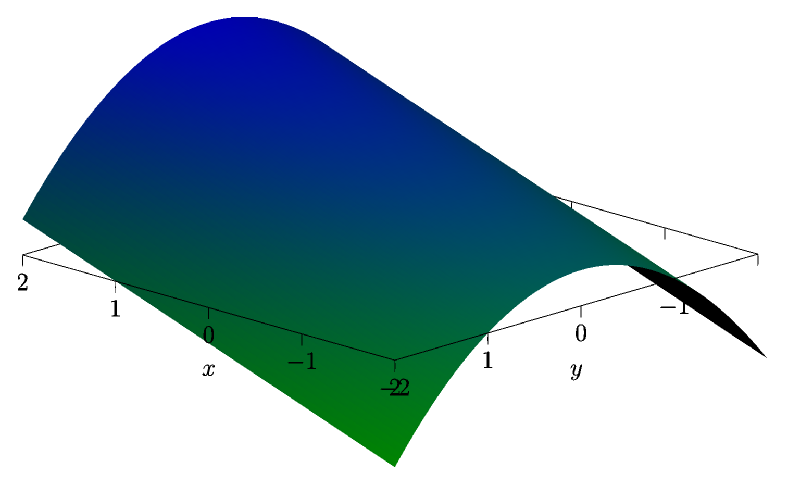
\includegraphics[width=12cm]{figure43.eps}
\caption{The function $f(x,y) = x-y^2+3$.}
\label{figure-3d-graph5}
\end{figure}

\begin{example}
For example, consider the function $f(x,y) = x-y^2+3$, shown in
Figure \ref{figure-3d-graph5}. We have $f_y(x,y) = -2y$, which
vanishes everywhere along the $x$ axis (when $y=0$). However,
the other partial is $f_x = 1$, which never vanishes. This
means that all points $(x,0)$ are potentiall critical in $y$
but not in $x$. What you get with this function is a
ascending/decending ridge (with slope $1$) above the $x$ axis.
\end{example}

\begin{figure}[t]
\centering
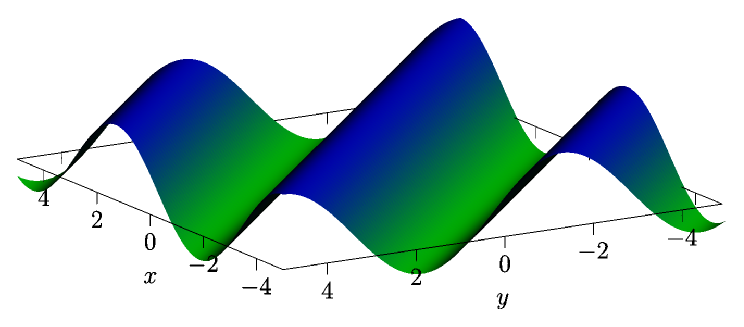
\includegraphics[width=12cm]{figure44.eps}
\caption{The function $f(x,y) = \cos (x+y)$}
\label{figure-3d-graph6}
\end{figure}

\begin{example}
Since we work in several dimensions, we can have very
complicated sets of maxima/minima. The function $f(x,y) = \cos
(x+y)$, shown in Figure \ref{figure-3d-graph6} has a maximum whenever
$x+y$ is an even multiple of $\pi$. Each of those sets is a
whole line, $x+y=0$, $x+y = 2\pi$ and so on. For functions of
two variables, its easy to have lines or curves of maximum or
minimum points. In higher dimensions, we can have surfaces or
hypersurfaces of maximum or minimum points.
\end{example}

We want to classify critical points: points where $\nabla f =
0$. We can do this informally by looking at each variable
individually. If the point is a maximum in all of $x_1, x_2,
\ldots, x_n$, then it is a maximum according to our definition
above. Likewise, if it is a minimum in all the variables, it
is a minimum. If it is a maxmum in some of the variables and a
minimum in others, it is a saddle point. However, if even one
of the variable has no max/min behvaiour (like $f(x) = x^3$ at
$x=0$), then the point is neither a maximum, minimum nor
saddle point.

\subsection{Hessian Matrices}
\label{hessians}

This informal approach is reasonable, but it would be nice to
have a more formal method for determining the behaviour. In
single variable calculus, we have the second-derivative test.
If $a$ is a critical point, then it is a maximum if
$f^{\prime \prime}(a)$ is negative, a minimum if $f^{\prime
\prime}(a)$ is positive, and the test is inconclusive if
$f^{\prime \prime}(a) = 0$. 

We'd like to generalize this, but we have many second
derivatives: all of the possible mixed and non-mixed second
partials. One way we can organize all these second partials
is in a matrix.

\begin{defn}
The matrix of all the second partial derivatives of a scalar
function $f$ is called the \emph{Hessian Matrix}. 
\end{defn}

Here is the Hessian matrix for $f(x,y)$ in two variables. 
\begin{equation*}
\left( \begin{matrix}
\dfrac{\del^2 f}{\del x^2} &
\dfrac{\del^2 f}{\del y \del x} \vspace{0.3cm}\\
\dfrac{\del^2 f}{\del x \del y} &
\dfrac{\del^2 f}{\del y^2}
\end{matrix} \right) 
\end{equation*}
Here is the Hessian matrix for $f(x,y,z)$ in three variables. 
\begin{equation*}
\left( \begin{matrix}
\dfrac{\del^2 f}{\del x^2} &
\dfrac{\del^2 f}{\del y \del x} &
\dfrac{\del^2 f}{\del z \del y} \vspace{0.3cm}\\
\dfrac{\del^2 f}{\del x \del y} &
\dfrac{\del^2 f}{\del y^2} &
\dfrac{\del^2 f}{\del z \del y} \vspace{0.3cm}\\
\dfrac{\del^2 f}{\del x \del z} &
\dfrac{\del^2 f}{\del y \del z} &
\dfrac{\del^2 f}{\del z^2} 
\end{matrix} \right) 
\end{equation*}
Note that the Hessian is not the Jacobian matrix from before;
that matrix had only first derivatives. The Hessian matrix
only applies to single valued function (outputs in $\RR$), is
always square, and lists all the possible second partials. 

The Hessian matrix captures all of the information about the
second derivative of this function, but it is often too
unwieldy to be used to determine the behaviour of critical
points. However, we have a useful tool from linear algebra to
get specific information out of a matrix: the determinant. Let
$D$ be the determinant of the Hessian matrix. For $f(x,y)$,
$D$ has the following form (using Clairaut's theorm to
simplify the mixed partials). 
\begin{equation*}
D = \frac{\del^2 f}{\del x^2} \frac{\del^2 f}{\del y^2} -
\left( \frac{\del^2 f}{\del x \del y} \right)^2
\end{equation*}
For functions of two variables, the determinant of the Hessian
tells us most of what we need to know.

\begin{prop}
Let $f: \RR^2 \rightarrow \RR$ be a $C^2$ function and let
$(a,b)$ be a critical point. Then we have four cases.
\begin{smallitemize}
\item If $D(a,b) > 0$ and $\frac{\del^2 f}{\del x^2} (a,b) >
0$ then the critical point is a minimum.
\item If $D(a,b) > 0$ and $\frac{\del^2 f}{\del x^2} (a,b) < 0$ then
the critical point is a maximum.
\item If $D(a,b) < 0$ then the critical point is a saddle
point.
\item If $D(a,b) = 0$ then the test is inconclusive.
\end{smallitemize}
\end{prop}

This proposition can be generalized to higher dimensions, but
it requires more machinery from linear algebra, namely
eigenvalues. Clairaut's theorem means that the Hessian is
always a symmetric matrix, so it always has a maximal set of
real eigenvalues. The general proposition classifies the
extrema using those eigenvalues.

\begin{prop}
Let $f: \RR^n \rightarrow \RR$ be a $C^2$ function with $H$
its Hessian matrix. Let $u \in \RR^n$ be a critical point and
let $H(u)$ be the Hessian evaluated at the point $u$. Then we
have four cases.
\begin{smallitemize}
\item If $H(u)$ is not invertible (has determinant 0, has 0 as
an eigenvalue), then the test is inconclusive. 
\item If all the eigenvalues of $H(u)$ are positive, then the
critical point is a local minimum.
\item If all the eigenvalues of $H(u)$ are negative, then the
critical point is a local maximum.
\item If the eigenvalues of $H(u)$ are a mix of positive and
negative, then the critical point is a saddle point.
\end{smallitemize}
\end{prop}

\subsection{Global Extrema}
\label{global-extrema}

\begin{figure}[t]
\centering
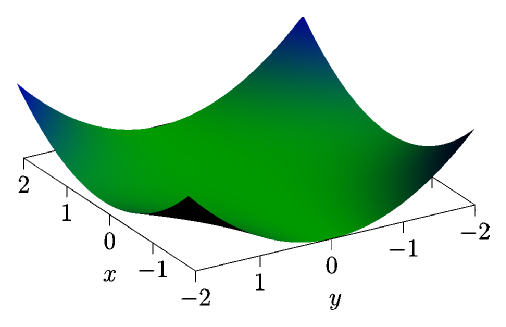
\includegraphics[width=12cm]{figure45.eps}
\caption{The function $f(x,y) = y^2x^2 + y^2$.}
\label{figure-3d-graph7}
\end{figure}

The above analysis was all about local maxima and minima. We
can also ask for global maxima and minima. Like the single
variable case, we do this by looking at all the local extrema
as well as the boundary. The maximum or minimum might be a
boundary point which is not a critical point. We do have an
existence proposition, which relies on the topology of the
domain. 

\begin{prop}
Let $C$ be closed set in $\RR^n$ and $f: C \rightarrow R$.
Then $f$ has at least one global maximum and at least one
global minimum, either at a local maximum/minimum or on its
boundary.
\end{prop}

In general, finding the maximum and minimum on the boundary
can be quite difficult. In the next section, we'll 
give another technique for finding such maxima and minima.

\begin{example}
$f(x,y) = y^2 x^2 + y^2$ is shown in Figure \ref{figure-3d-graph7}.
\begin{align*}
\frac{\del f}{\del x} & = 2xy^2 \\
\frac{\del f}{\del y} & = 2yx^2 + 2y \\
\nabla f(x,y) & = 0 \implies (x,y) = (a,0) \hspace{1cm}
\forall a \in \RR 
\end{align*}

\begin{align*}
\frac{\del^2 f}{\del x^2} & = 2y \hspace{2cm}
\frac{\del^2 f}{\del y^2} = 2x^2 + 2 \hspace{2cm}
\frac{\del^2 f}{\del x \del y} = 4xy \\
D & = (2y)(2x^2+ 2) - 16x^2 y^2 = 4yx^2 + 4y - 16x^2 y^2
\implies D(a,0) = 0
\end{align*}
At all the critical points $(a,0)$, the second derivative test
has $D=0$, which is inconclusive. We have to investigate
directly. We can see that $f(a,0) = 0$. But $f(a,b)$ for $b$
any small non-zero nubmer takes the value $a^2 b^2 + b^2$,
which is always positive. Therefore, we can conclude that all
the critical points $(a,0)$ are local minima. In Figure
\ref{figure-3d-graph7}, we can see that all along the $y$ axis the
values stay at $0$, which is the lowest output of the
function.
\end{example}

\begin{figure}[t]
\centering
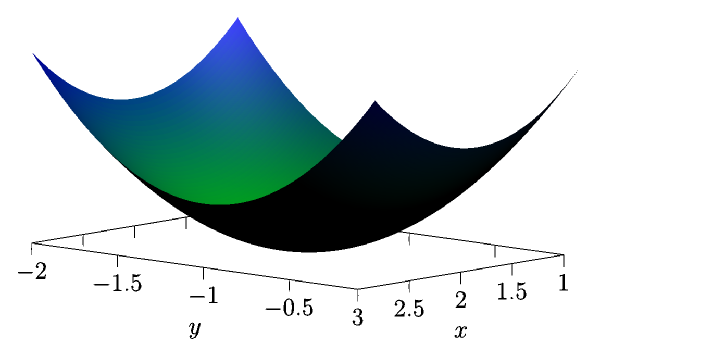
\includegraphics[width=12cm]{figure46.eps}
\caption{The function $f(x,y) = x^2+2y^2 - 4x + 4y + 6$.}
\label{figure-3d-graph8}
\end{figure}

\begin{example}
$f(x,y) = x^2 + 2y^2 - 4x + 4y + 6$ is shown in Figure
\ref{figure-3d-graph8}. 
\begin{align*}
\frac{\del f}{\del x} & = 2x-4 \\
\frac{\del f}{\del y} & = 4y+4 \\
\nabla f(x,y) & = 0 \implies (x,y) = (2,-1) \\
\frac{\del^2 f}{\del x^2} & = 2 > 0 \\
\frac{\del^2 f}{\del y^2} & = 4 > 0 \\
\frac{\del^2 f}{\del x \del y} & = 0 \\
D & = 8 > 0 
\end{align*}
The point $(2,-1)$ is a local minimum.
\end{example}

\begin{figure}[t]
\centering
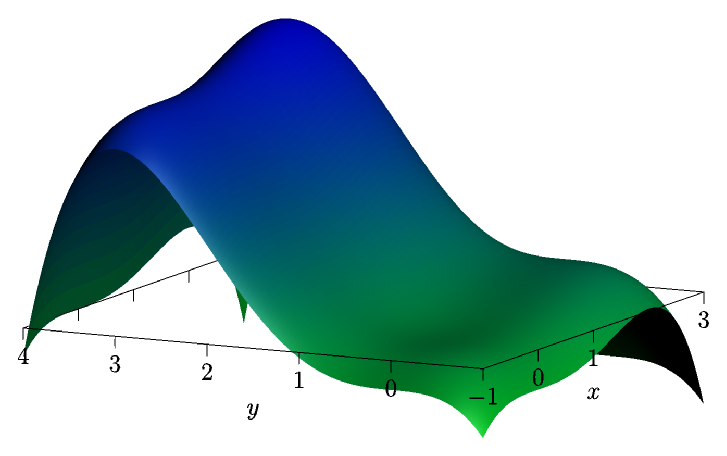
\includegraphics[width=12cm]{figure47.eps}
\caption{The function $f(x,y) =\frac{8}{3}x^3 + 4y^3 - x^4 -
y^4$.}
\label{figure-3d-graph9}
\end{figure}

\begin{example}
$f(x,y) = \frac{8}{3} x^3 + 4y^3 - x^4 - y^4$ is shown in
Figure \ref{figure-3d-graph9}
\begin{align*}
\frac{\del f}{\del x} & = 8x^2 - 4x^3 = 4x^2 (2-x) \\
\frac{\del f}{\del y} & = 12y^2 - 4y^3 = 4y^2 (3-y) \\
\nabla f(x,y) & = 0 \implies (x,y) = (0,0), (0, 3), (2, 0),
(2,3) \\
\frac{\del^2 f}{\del x^2} & = 16x - 12x^2 = 3x(4-3x) \\
\frac{\del^2 f}{\del y^2} & = 24y - 12y^2 = 12(2-y) \\
\frac{\del^2 f}{\del x \del y} & = 0 \\
D & = 48xy (4-3x)(2-y)\\
D(0,0) & = 0 \hspace{1cm}
D(0,3) = 0 \hspace{1cm}
D(2,0) = 0 \hspace{1cm}
D(2,3) > 0 \hspace{1cm}
\frac{\del^2 f}{\del x^2} (2,3) < 0 
\end{align*}
The point $(2,3)$ is a local maximum, but the test
is inconclusive at all other points. As we can see in Figure
\ref{figure-3d-graph9}, there is a maximum above $(2,3)$. At the other
three critical points, we can observe a momentary flattening
of the graph, but we have neither maxima, minima, nor saddle
points. The zero Hessian for these points makes sense; they
are like the critical point at $x=0$ of the cubic $f(x) =
x^3$, which has a zero derivative, but no extremum.
\end{example}

\begin{example}
\label{example-box-sphere}
Let's try a more geometric optimization problem: what is the
largest rectangular prism you can fit in a sphere of radius
$r$? We'll assume that the prism is centrally located in the
sphere, which means that its shape is entirely determined by
one of its vertices on the edge of the sphere. If that vertex
is $(x,y,z)$, then the volume of the prism is $2x \times 2y
\times 2z$. 

I'd like to work in spherical coordinates instead of $x$, $y$
and $z$. The radius $r$ is fixed, but $\theta$ (longitude) and
$\phi$ (colatitude) will vary. 
\begin{align*}
h & = 2r \cos \phi \\
w & = 2r \sin \phi \cos \theta \\
l & = 2 r \sin \phi \sin \theta \\
V & = hwl = 8r^3 \cos \phi \sin^2 \phi \cos \theta \sin \theta
= 4 r^3 \sin (2\theta) (\cos \phi - \cos^3 \phi)
\end{align*}
Then we can optimize the function $V(\theta, \phi)$.
\begin{align*}
\frac{\del V}{\del \phi} & = 4r^3 \sin (2\theta) (- \sin \phi
+ 3 \cos^2 \phi \sin \phi) \\
\frac{\del V}{\del \theta} & = 8r^3 \cos 2 \theta (\cos \phi -
\cos^3 \phi) \\
\nabla V & = 0 \implies (\phi, \theta) = \left( \arccos
\frac{1}{\sqrt{3}}, \frac{\pi}{4} \right) \\
V & = 4t^3 \sin \frac{\pi}{2} \left( \frac{1}{\sqrt{3}} -
\frac{1}{3\sqrt{3}} \right) = \frac{8r^3}{3\sqrt{3}}
\end{align*}
We didn't do the calcluation, but it is reasonable to check that the
critical point represents a maximum. The area we get is the
area of cube of side length $\frac{2r}{\sqrt{3}}$, which
seems, intuitively, like the right kind of length. 
\end{example}

\section{Constrained Optimization}
\label{constrained-optimization}

Let's reconsider the box-in-a-sphere problem of Example
\ref{example-box-sphere}. Instead of
working inside the sphere, we could just consider a prism
centred at the origin with positive octant vertex $(a,b,c)$
and volume $8abc$. That maximized by itself will diverge to
$\infty$, since we have nothing to bound the prism. However,
we can consider the \emph{constraint} $x^2 + y^2 + z^2 = r^2$
for some fixed $r$. 

The idea, in general, is to ask when a function $f(x_1, x_2,
\ldots, x_n)$ is optimized subject to one (or more)
constraints $g(x_1, x_2, \ldots x_n) = c$. Let's first think
of this geometrically. If both $f$ and $g$ were functions of
two variables, we could draw contour plots. $g(x,y) = c$
would be a fixed countour line for $g$, and we would be asking
for maximum of $f$ along that contour line. We can notice
that such a maximum occurs where a countour line for $f$
touches the contour line $g(x,y) = c$ and then backs off. That
is, the maximum occurs where the contour lines are tangent. 

But the contour lines are level sets, which are defined by
their normals. The normals are given by gradients. If the
level sets are tangent to each other, that means the gradients
must be in the same direction (up to a sign). That is, this
optimization occurs when $\nabla f \parallel \nabla g$. We can
express this as $\nabla f = \lambda \nabla g$ for some real
constant $\lambda \neq 0$.

This holds in any dinemsion: the level sets will be
tangent and there will be a constant $\lambda$ with $\nabla f
= \lambda \nabla g$. To optimize with constraint, we now have
a system of equation in $n+1$
variables, the $x_i$ and $\lambda$: $\nabla f = \lambda \nabla
g$ and $g(x_1, x_2, \ldots, v_n) = c$. To optimize the
situation, we try to solve this system. This method is called
the method of Lagrange Multipliers.

(Historically, the connection to the mathematician Lagrange
comes from a \emph{Lagrangian} of the form $f + \lambda g$.
We're essentially looking for critical points of this
Lagrangian).

\begin{example}
What is the largest rectangle with fixed perimeter $p$? The
rectangle has length $l$ and height $h$, with area $A(h,l) =
hl$. The constraint is the fixed perimeter $2h + 2l = p$, so
the function is $g(h,l) = 2h + 2l$. The gradients are $\nabla
A = (l,h)$ and $\nabla g = (2,2)$. The equation $\nabla A =
\lambda \nabla g$ is two equations: $h = 2\lambda$ and $l = 2
\lambda$. We can substitute these into the constrait $2h + 2l
= p$ to get $8 \lambda = p$ so $\lambda = p/8$ and $h = l = 2
\lambda = p/4$.  The area is then $p^2/16$.
\end{example}

\begin{example}
Let's actually do the motivating Example \ref{example-box-sphere} with
Lagrange Multipliers. 
\begin{displaymath}
\begin{array}{*4{>{\displaystyle}l}}
V(x,y,z) = 8xyz & & 
\hspace{1cm} g(x,y,z) = x^2 + y^2 + z^2 = r^2 & \\[1em]
\nabla V = (8yx,8xz,8xy) & & 
\hspace{1cm} \nabla g = (2x, 2y, 2z) & \\[1em]
\nabla V = \lambda \nabla g & & & \\[1em]
8yz = \lambda 2x & 
\hspace{1cm} 8xz = \lambda 2y & 
\hspace{2cm} 8xy = \lambda 2z & 
\end{array}
\end{displaymath}
We will use the first of the three equations to isolate for
$x$, which we substitute in the second. 
\begin{align*}
x & = \frac{1}{\lambda} 4yz 
\hspace{1cm} \frac{8}{\lambda} 4yz^2 = \lambda 2y \\
\intertext{We solve for $z$ (cancelling $y$, so careful with
the possibility of $y=0$.)}
16z^2 & = \lambda^2 \implies z = \frac{\lambda}{4} \\
\frac{8}{\lambda} 4 y^2 z & = \lambda 2z \\
\intertext{Since everything in this question is symmetric, we
apply the same reasoning with different variables.}
y & = \frac{\lambda}{4} \hspace{2cm} 
x = \frac{\lambda}{4} \\
\intertext{We put $x$, $y$ and $z$ into the constraint to
solve for $\lambda$.}
x^2 + y^2 + z^2 & = \frac{3\lambda^2}{16} = r^2 \implies 
\lambda = \frac{4r}{\sqrt{3}} \\
\intertext{Then we use the value of $\gamma$ to give the
values of the variables.}
x = y = z & = \frac{r}{\sqrt{3}} \\
V & = \frac{8r^3}{3\sqrt{3}}
\end{align*}
We recovered the same maximal area as before. We don't have to
worry about the $y=0$ possibility that we noted (or likewise
$x=0$ and $z=0)$, since any solution in that case would lead
to zero volume, which is certainly not maximal. 
\end{example}

\begin{example}
Instead of a sphere, we could ask for the largest box inside
an ellipsoid with equation $\frac{x^2}{a^2} + \frac{y^2}{b^2}
+ \frac{z^2}{c^2} = 1$. Geometrically, this because more
difficult. However, using Lagrange Multipliers, we only need
to change the constraint from the equation of the sphere to
the equation of the ellipse.
\begin{displaymath}
\begin{array}{*4{>{\displaystyle}l}}
V(x,y,z) = 8xyz & & 
\hspace{1cm} g(x,y,z) = \frac{x^2}{a^2} + \frac{y^2}{b^2} +
\frac{z^2}{c^2} = r^2 & \\[1em]
\nabla V = (8yx,8xz,8xy) & & 
\hspace{1cm} \nabla g = \left( \frac{2x}{a^2}, \frac{2y}{b^2},
\frac{2z}{c^2} \right) & \\[1em]
\nabla V = \lambda \nabla g & & & \\[1em]
8yz = \lambda \frac{2x}{a^2} &
\hspace{1cm} 8xz = \lambda \frac{2y}{b^2} &
\hspace{2cm} 8xy = \lambda \frac{2z}{c^2} \\
\end{array}
\end{displaymath}
We isolate for $x$ in the first expression and substitute in
the second.
\begin{align*}
x & = \frac{4z^2 yz}{\lambda} \hspace{2cm}
8 \left( \frac{4a^2yz}{\lambda} \right) z = \frac{\lambda
2y}{b^2} \\
\intertext{We solve for $z$ (again, careful with $y=0$).}
16a^2 b^2 z^2 & = \lambda^2 \implies
4abz = \lambda \implies 
z = \frac{\lambda}{4ab} \\
\intertext{We have symmetry again in the variables.}
x & = \frac{\lambda}{4bc} \hspace{2cm}
y = \frac{\lambda}{4ac} \\
\intertext{We substitute $x$, $y$ and $z$ in the constraint
and solve for $\lambda$.}
\frac{x^2}{a^2} + \frac{y^2}{b^2} +
\frac{z^2}{c^2} & = 3 \left( \frac{\lambda^2}{16a^2b^2c^2}
\right) = 1 \implies
\lambda = \frac{4abc}{\sqrt{3}} \\
\intertext{We use the value of $\lambda$ to determine the
other variables.}
x & = \frac{a}{\sqrt{3}} \hspace{2cm}
y = \frac{b}{\sqrt{3}} \hspace{2cm}
z = \frac{c}{\sqrt{3}} \\
V & = \frac{8abc}{3\sqrt{3}}
\end{align*}
The volume of the ellipsoid is $\frac{4}{3} \pi abc$, so as a
fraction of that volume, this is $\frac{2}{\sqrt{3}\pi}$ times
the volume of the ellipse, a very believable fraction. Again,
the $x=0$, $y=0$ or $z=0$ cases are discounted since they
would lead to zero area and we are looking for a maximum. 
\end{example}

\begin{example}
We can use Lagrange multipliers with several constraints for
higher dimensional problems. Consider a plane $x +y+ z = 12$
and a parabaloid $z = x^2 +y^2$. Their intersection is an
ellipse in $\RR^3$. I'd like to find its highest point and its
lowest point, thinking of $z$ as elevation. In Lagrange
Multipliers, rhe function $f(x,y,z) = z$ is simply height, and
the two equations are the constraints. 
\begin{displaymath}
\begin{array}{*3{>{\displaystyle}l}}
f(x,y,z) = z &
\hspace{1cm} g(x,y,z) = x + y + z = 11 &
\hspace{1cm} h(x,y,z) = x^2 + y^2 - z = 0 \\
\nabla f = (0,0,1) &
\hspace{1cm} \nabla g = (1,1,1) &
\hspace{1cm} \nabla h = (2x, 2y, -1) \\
\nabla f = \lambda \nabla g + \mu \nabla h & & \\
0 = \lambda + 2 x \mu &
\hspace{1cm} 0 = \lambda + 2y \mu &
\hspace{1cm} 1 = \lambda - \mu 
\end{array}
\end{displaymath}
This system is relatively straightforward, even with five
variables. We can solve for $\lambda$ in the first two
equation and equate the results.
\begin{align*}
2x\mu & = \lambda = 2 y \mu \implies x = y \ \ \ ( \mu \neq
0) \\
\intertext{We put $x$ and $y$ into the $h$ constraint.}
z & = 2x^2 \\
\intertext{Then we put this expressionv for $z$, and replace
$y$ with $x$ in the $g$ constraint. This result is an
expression solely in $x$, so we can solve for values of $x$.}
2x + 2x^2 & = 12 \implies x = -3 \text{ or } x = 2 \\
\intertext{We know the other variables in terms of $x$, so
values of $x$ determine values of $y$ and $z$. }
x & = -3 \implies y = -3 \ \ z = 18 \\
x & = 2 \implies y = 2 \ \ z = 8 
\end{align*}
We can simply look at the $z$ value, since we are trying to
maximize it. We see a maximum at $(-3, -3, 18)$ and the
minimum at $(2,2,8)$. 
\end{example}

\begin{example}
As we've seen in these examples, constrained optimization is a
particularly useful tool for sovling complicated geometry
problems. Here is another such problem.  Say we have the
equation of a very general ellipse centred at the origin, such
as $17x^2 + 12xy + 8y^2 = 100$. Since this ellipse has an $xy$
term, it is not oriented along any axis -- it's on some
slanted plane through the origin. So we don't know,
from inspection, what is major and minor semi-axes are.
However, we can ask for the points further from and closest
too the origin. That's asking for the min and max of the
funciton $f(x,y) = x^2 + y^2$ on the constraint which is the
equation of the ellipse.
\begin{displaymath}
\begin{array}{*2{>{\displaystyle}l}}
f(x,y) = x^2 + y^2 &
\hspace{2cm} g(x,y) = 17x^2 + 12xy + 8y^2 = 100 \\
\nabla f = (2x, 2y) &
\hspace{2cm} \nabla g = (34x + 12y, 12x + 16y) \\
\nabla f = \lambda \nabla g & \\
2x = \lambda( 34x + 12y) &
2y = \lambda( 12x + 16y) 
\end{array}
\end{displaymath}
We solve for $\lambda$ in both equation and equate the
results. 
\begin{align*}
\frac{-2x}{34x + 12 y} & = \lambda = \frac{-2y}{12 x + 16 y} \\
12x^2 + 16xy & = 34 xy + 12y^2 \\
\intertext{This is a bit tricky, since there are quadratic
terms in both $x$ and $y$. Turns out, though, we can get use
out of isolating $y^2$.}
2x^2 - 3xy - 2y^2 & = 0 \implies 
y^2 = x^2 - \frac{3}{2} xy \\
\intertext{We replace $y^2$ in the constraint. We are
fortunate, since this replacement cancelled off the $xy$ term
and leaves us just with an expression in $x$.}
12 x^2 + 12 xy + 8 \left( x ^2 - \frac{3}{2} xy \right) & =
100 \\
12x^2 + 8x^2 & = 100 \implies x = \pm 2 \\
x & = 2 \implies 8 - 6y - 2y^2 = 0 \implies y = 1, -4 \\
x & = -2 \implies 8 + 6y - 2y^2 = 0 \implies y = -1, 4 \\
\end{align*}
This gives us the four points $(2,1)$, $(-2,-1)$, $(2,-4)$ and
$(-2,4)$. The semi-major axis is the distance to the further
point, and the semi-minor axis is the distance to the closet
point (from the origin). Therefore, the semi-major axis is
$\sqrt{20}$ units long along the line in the direction
$(2,-4)$ and the semi-minor axis is $\sqrt{5}$ units long in
the direction $(2,1)$. 
\end{example}

\end{document}
